\documentclass[a4paper,12pt,twoside]{memoir}

% Castellano
\usepackage[spanish,es-tabla]{babel}
\selectlanguage{spanish}
\usepackage[utf8]{inputenc}
\usepackage[T1]{fontenc}
\usepackage{lmodern} % scalable font
\usepackage{microtype}
\usepackage{placeins}
\usepackage{rotating}

\RequirePackage{booktabs}
\RequirePackage[table]{xcolor}
\RequirePackage{xtab}
\RequirePackage{multirow}

% Links
\PassOptionsToPackage{hyphens}{url}\usepackage[colorlinks]{hyperref}
\hypersetup{
	allcolors = {red}
}

% Ecuaciones
\usepackage{amsmath}

% Rutas de fichero / paquete
\newcommand{\ruta}[1]{{\sffamily #1}}

% Párrafos
\nonzeroparskip

% Huérfanas y viudas
\widowpenalty100000
\clubpenalty100000

% Evitar solapes en el header
\nouppercaseheads


\let\tmp\oddsidemargin
\let\oddsidemargin\evensidemargin
\let\evensidemargin\tmp
\reversemarginpar



% Imagenes
\usepackage{graphicx}
\usepackage[style=numeric, sorting=none]{biblatex}
\addbibresource{bibliografiaAnexos.bib}
\newcommand{\imagen}[2]{
	\begin{figure}[!h]
		\centering
		\includegraphics[width=0.9\textwidth]{#1}
		\caption{#2}\label{fig:#1}
	\end{figure}
	\FloatBarrier
}






\graphicspath{ {./img/} }

% Capítulos
\chapterstyle{bianchi}
\newcommand{\capitulo}[2]{
	\setcounter{chapter}{#1}
	\setcounter{section}{0}
	\setcounter{figure}{0}
	\setcounter{table}{0}
	\chapter*{#2}
	\addcontentsline{toc}{chapter}{#2}
	\markboth{#2}{#2}
}

% Apéndices
\renewcommand{\appendixname}{Apéndice}
\renewcommand*\cftappendixname{\appendixname}

\newcommand{\apendice}[1]{
	%\renewcommand{\thechapter}{A}
	\chapter{#1}
}

\renewcommand*\cftappendixname{\appendixname\ }

% Formato de portada
\makeatletter
\usepackage{xcolor}
\newcommand{\tutor}[1]{\def\@tutor{#1}}
\newcommand{\tutorb}[1]{\def\@tutorb{#1}}
\newcommand{\course}[1]{\def\@course{#1}}
\definecolor{cpardoBox}{HTML}{E6E6FF}
\def\maketitle{
  \null
  \thispagestyle{empty}
  % Cabecera ----------------
\begin{center}
  \noindent
\includegraphics[width=\textwidth]{cabeceraSalud}\vspace{1.5cm}%
\end{center}
  
  % Título proyecto y escudo salud ----------------
  \begin{center}
    \begin{minipage}[c][1.5cm][c]{.20\textwidth}
        
\includegraphics[width=\textwidth]{escudoSalud.pdf}
    \end{minipage}
  \end{center}
  
  \begin{center}
    \colorbox{cpardoBox}{%
        \begin{minipage}{.8\textwidth}
          \vspace{.5cm}\Large
          \begin{center}
          \textbf{TFG del Grado en Ingeniería de la Salud}\vspace{.6cm}\\
          \textbf{\LARGE\@title{}}
          \end{center}
          \vspace{.2cm}
        \end{minipage}
    }%
  \end{center}
  
    % Datos de alumno, curso y tutores ------------------
  \begin{center}%
  {%
    \noindent\LARGE
    Presentado por \@author{}\\ 
    en Universidad de Burgos\\
    \vspace{0.5cm}
    \noindent\Large
    \@date{}\\
    \vspace{0.5cm}
    %Tutor: \@tutor{}\\ % comenta el que no corresponda
    Tutor: \@tutor{}\\
  }%
  \end{center}%
  \null
  \cleardoublepage
  }
\makeatother



% Datos de portada
\title{Solución tecnológica para la monitorización de síntomas motores en pacientes con Párkinson \\Documentación Técnica}
\author{Carmen Marcos Gordillo}
\tutor{Guirguis Zaki Guirguis Abdelmessih}
\date{\today}

\begin{document}

\maketitle



\cleardoublepage



%%%%%%%%%%%%%%%%%%%%%%%%%%%%%%%%%%%%%%%%%%%%%%%%%%%%%%%%%%%%%%%%%%%%%%%%%%%%%%%%%%%%%%%%



\frontmatter


\clearpage

% Indices
\tableofcontents

\clearpage

\listoffigures

\clearpage

\listoftables

\clearpage

\mainmatter

\appendix




\apendice{Plan de Proyecto Software}

\section{Introducción}
Es esencial realizar al inicio de cada proyecto una planificación temporal del desarrollo del mismo, un presupuesto estimado del coste que va a suponer y un análisis de la normativa vigente que afecta a la viabilidad del mismo en el territorio correspondiente. Para ello se detallan en el presente anexo 3 secciones relativas a estas planificaciones.

\section{Planificación temporal}
La evolución del proyecto fue documentada mediante la utilización de GitHub, aplicación en la cual se definieron 6 milestones u objetivos principales del desarrollo del proyecto. Algunos de estos milestones se dividieron en diferentes issues:
\begin{itemize}
    \item Desarrollo de aplicación web
    \begin{itemize}
        \item Generación de informe descargable (incluye generación de gráficas básicas sobre las actividades)
        \item Personalización de tiempo de bloqueo (parte 1 y parte 2)
        \item Creación de un diario de fluctuaciones motoras
        \item Almacenamiento de datos del diario en la base de datos
        \item Registro de fecha y hora de las actividades realizadas
        \item Creación de gráficas que relacionen las fluctuaciones motoras con la toma de medicaciones y los bloqueos/min en actividades.
        \item Desarrollo front-end para el acceso a nuevas funciones desde la página web
    \end{itemize}
    \item Configuración del hardware
    \begin{itemize}
        \item Diseño de hardware nuevo
        \item Creación de nuevo hardware
        \item Pruebas de hardware
        \item Inserción de hardware en soporte flexible
    \end{itemize}
    \item Actualizaciones del código Arduino
    \begin{itemize}
        \item Adaptación del código Arduino al módulo láser
        \item Corrección del registro de duración total de las actividades
    \end{itemize}
    \item Redacción de memoria del proyecto: Este milstone abarca la redacción de los diferentes apartados de la memoria: Introducción, objetivos, conceptos teóricos, metodología, conclusiones y líneas futuras.
    \item Redacción de Anexos: Este milestone abarca la redacción de los diferentes Anexos (Anexo A- Anexo H).
    \item Elaboración de presentación para la defensa del proyecto
\end{itemize}
Debido a la naturaleza de la metodología iterativa utilizada, el cumplimiento de estos objetivos generales se realizó de forma simultánea a lo largo del desarrollo del proyecto. Los cambios en el código fueron actualizados en la plataforma Github mediante el software Github Desktop, mientras que los documentos redactados fueron redactados a lo largo del desarrollo del proyecto e incluidos en el repositorio al final del mismo.

El cumplimiento de cada tarea que compone los diferentes objetivos se planificó de manera inicial mediante el desarrollo del diagrama de Gantt mostrado en la figura \ref{fig:Diagramagantt}. Sin embargo, el cumplimiento real de esta planificación se refleja en el diagrama de Gantt mostrado en la figura \ref{fig:Diagramagantt2}.

\begin{sidewaysfigure}
    \centering
    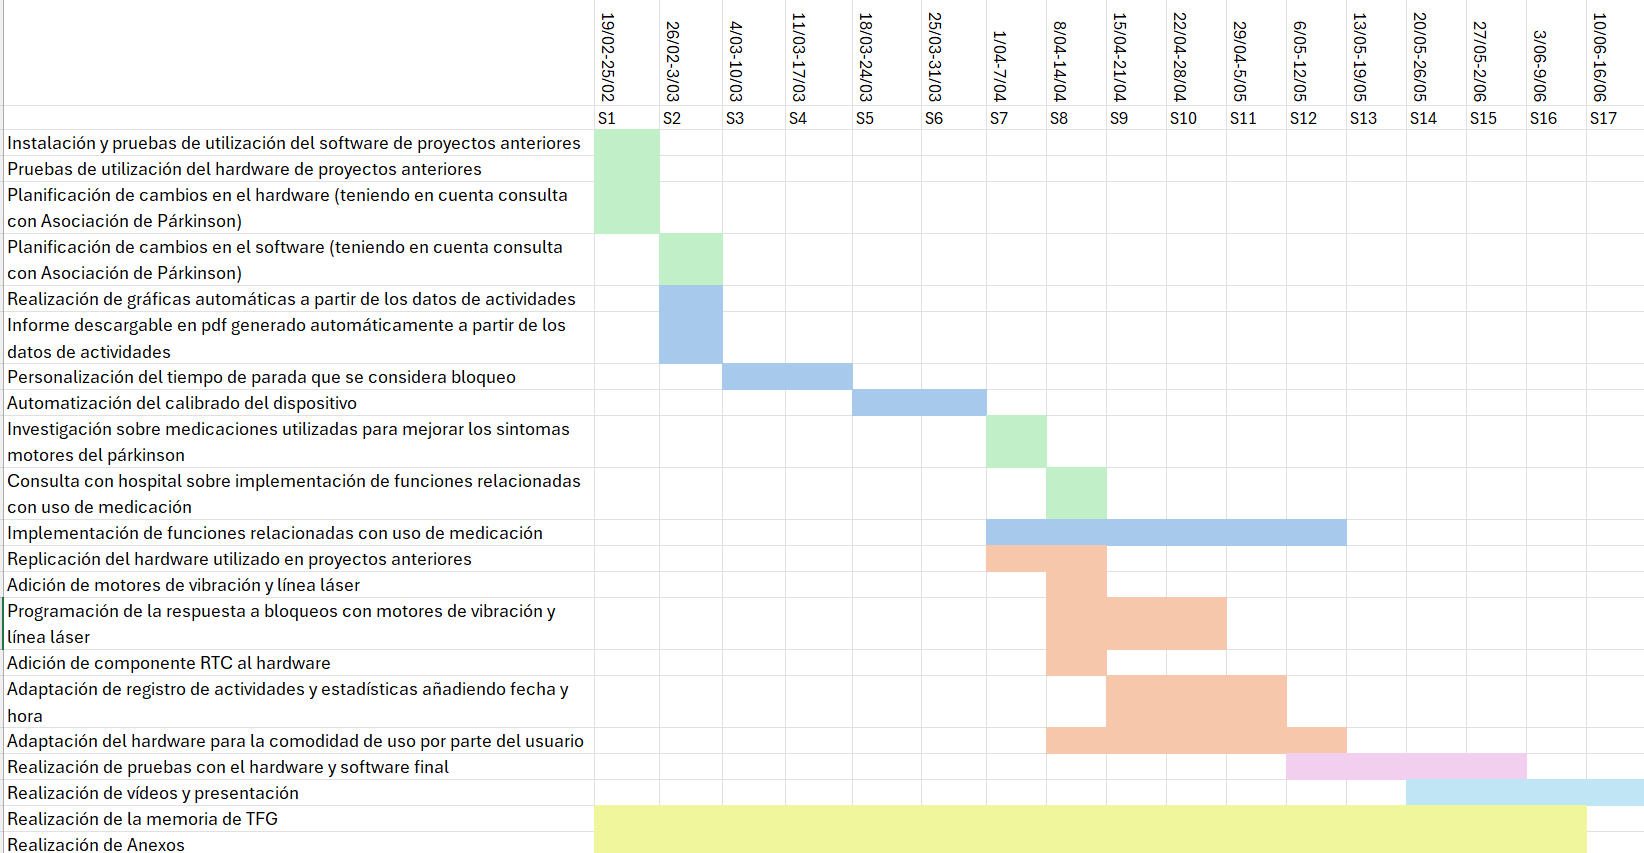
\includegraphics[width=1\textwidth]{img/gant1.png}
    \caption{Diagrama de Gantt: planificación temporal inicial del proyecto}
    \label{fig:Diagramagantt}
\end{sidewaysfigure}

\begin{sidewaysfigure}
    \centering
    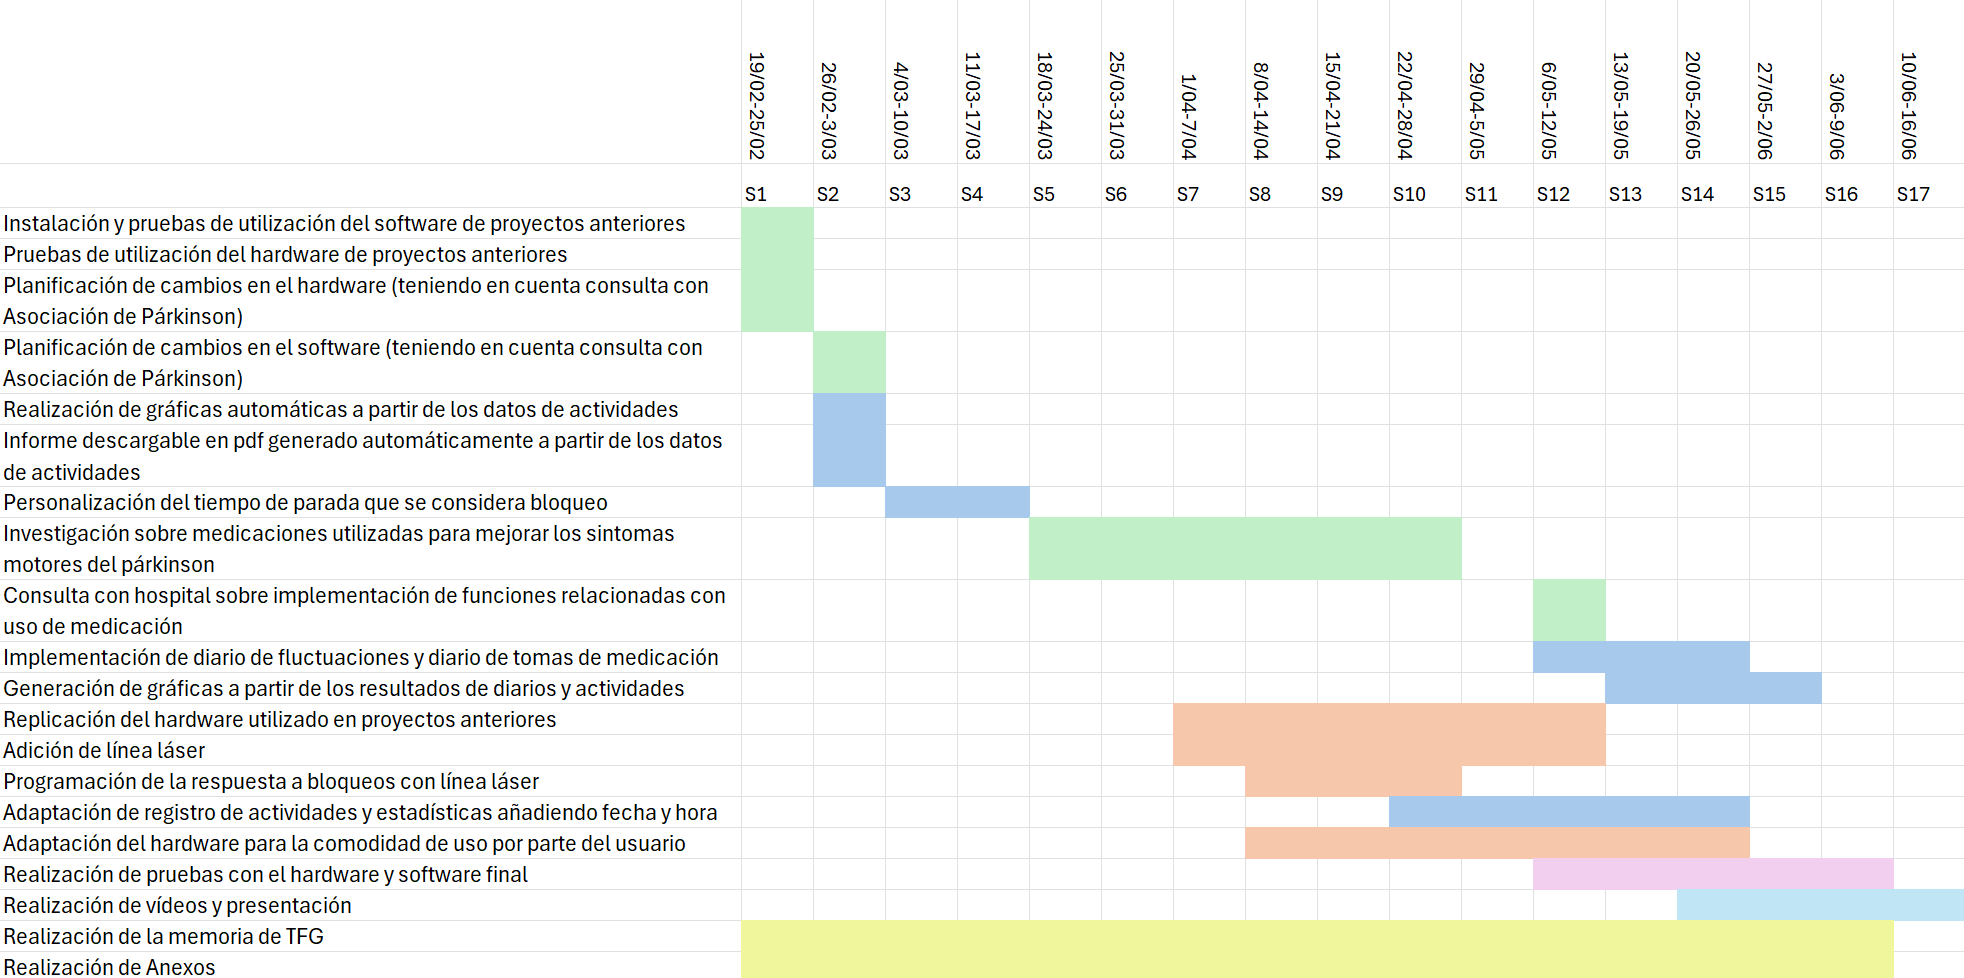
\includegraphics[width=1\textwidth]{img/gant2.png}
    \caption{Diagrama de Gantt: planificación temporal final del proyecto}
    \label{fig:Diagramagantt2}
\end{sidewaysfigure}

\section{Planificación económica}
El coste total de el proyecto, incluyendo costes de personal, software, hardware, amortización del ordenador utilizado y materiales es de aproximadamente 4982.3 euros. A continuación se describen en detalle cada uno de estos costes.
\subsection{Costes de personal}
El sueldo medio del ingeniero biomédico junior (con 0 a 3 años de experiencia) en España es de 29.020 € brutos por año \cite{jobted-ingeniero-biomedico}. Las horas empleadas en la realización del proyecto son equivalentes a 4 meses de trabajo con jornada parcial o 2 meses a jornada completa. Esto hace que el coste de personal durante la realización del proyecto sea de unos 4836,7€ brutos.
\subsection{Costes del software utilizado}
El software utilizado fue de código abierto, gratuito o facilitado con los paquetes disponibles para estudiantes de la Universidad de Burgos, por lo que el proyecto no presentó costes de software. A continuación se desglosa la naturaleza de las herramientas software utilizadas (descritas en el apartado 'Metodología' de la memoria de este proyecto) y el motivo de la gratuidad de su uso:
\begin{itemize}
    \item XAMPP: software de código abierto, licencia Apache 2.0: uso, modificación y redistribución gratuitos.
    \item Visual Studio Code: software gratuito con licencia MIT: gratuito para su uso y distribución. 
    \item IDE Arduino: software de código abierto  con licencia GNU LPGL (Lesser General Public License): gratuito para su uso y redistribución, con libertad para modificar el código fuente.
    \item Autodesk Sketchbook: versión gratuita para el uso personal y educativo.
    \item Microsoft Visio y Microsoft Excel: Incluidos en el paquete de Microsoft 365 ofrecido de forma gratuita a los estudiantes de la Universidad de Burgos.
    \item Versión 2 de ChatGPT: uso gratuito, sujeto a los términos y condiciones de OpenAI.
    \item Lucidchart: Versión gratuita con funciones limitadas.
    \item Balsamiq Wireframes: Software comercial que requiere licencia de compra o suscripción para su uso. Se utilizó la prueba gratuita del mismo.
    \item Visual Paradigm: Versión gratuita para uso personal y académico.
    \item Tinkercad: Versión gratuita para uso personal, educativo y comercial (este último siguiendo los términos de servicio de Autodesk).
\end{itemize}
\subsubsection{Costes del hardware y materiales utilizados}

En la tabla \ref{tab:preciomateriales} se desglosa el coste de cada material y herramienta hardware utilizados en el proyecto. El coste total de estos materiales supone 89.8 euros para la construcción de un prototipo.


\begin{table}[]
\begin{tabular}{
>{\columncolor[HTML]{DAE8FC}}l 
>{\columncolor[HTML]{EFEFEF}}l }
\cellcolor[HTML]{C0D5E5}Material/hardware & \cellcolor[HTML]{C0D5E5}Precio \\
Microcontrolador Arduino UNO R3           & 28 euros                       \\
Sensor MPU-6050                           & 5.99 euros                     \\
Pantalla LCD 16x2 con módulo LCD I2C      & 4.99 euros                     \\
2 pulsadores                              & 0.06 euros                     \\
Módulo láser                              & 4.99 euros                     \\
Módulo bluetooth HC-05                    & 9.99 euros                     \\
Interruptor ON/OFF                        & 3.99 euros                     \\
Conector aviación 4 pines                 & 1.77 euros                     \\
1m Cable multihilo 4 núcleos              & 2.39 euros                     \\
2m cable                                  & 0.42 euros                     \\
Fuente de alimentación recargable 9V      & 9.99 euros                     \\
Miniplaca de pruebas para Arduino         & 1.33 euros                     \\
Cable adaptador de batería Arduino DC 9V  & 3.90 euros                     \\
Riñonera/cinturón deportivo               & 11.99 euros                   
\end{tabular}
\label{tab:preciomateriales}
\caption{Desglose de los costes de materiales y hardware}
\end{table}

\subsection{Amortización de los equipos}
Se ha utilizado un dispositivo LG Gram 17ZD90R Intel Core i7-1360P/16GB. El coste de este dispositivo ha sido de 1172€, y se estima una vida útil de 7 años.
La amortización lineal de un producto puede estimarse mediante la siguiente fórmula \cite{liberto2024straightline}:

\text{Amortización lineal} = (\text{Precio de Compra del Activo} - \text{Valor Residual})/ \text{Vida Útil Estimada del Activo}

Con el objetivo de calcular la amortización lineal mensual del dispositivo utilizado, se utiliza por tanto la siguiente fórmula:

\text{Amortización lineal mensual} = (\text{Precio de Compra del Activo} - \text{Valor Residual})/ \text{Vida Útil Estimada del Activo en meses}

\text{Amortización lineal mensual} = (\text{1172€} - \text{0€})/84 \text{ meses} = \text{13,95€/mes}

Se calculará la amortización lineal del dispositivo en un periodo de tiempo de 4 meses:

\text{Amortización lineal total} = \text{13.95€/mes}* \text{4 meses}= 55.8€

\subsection{Viabilidad legal}
Con el objetivo de garantizar el cumplimiento del proyecto con las normas establecidas para dispositivos médicos y aplicaciones relacionadas con la salud en España, es importante tener en cuenta una serie de normativas a nivel europeo y nacional relacionadas con la comercialización de dispositivos médicos y la protección de datos, las cuales se exponen a continuación:
\subsubsection{Comercialización de dispositivos médicos}
Acorde con el Reglamento (UE) 2017/745 \cite{reglamento-ue-2017-745}, tanto la aplicación web como el dispositivo presentados en el presente proyecto entran dentro de la categoría de productos sanitarios. Este reglamento clasifica los dispositivos médicos en diferentes clases según su riesgo, requiriendo los dispositivos pertenecientes a cada clase diferentes procedimientos para la evaluación de conformidad. 

El presente dispositivo pertenercería a la clase I o clase de riesgo bajo, compuesta por los dispositivos que no están en contacto invasivo con el cuerpo o tan sólo están en contacto externo con la piel intacta, como es el caso del dispositivo presentado. Pertenecer a esta clase simplifica significativamente el proceso de comercialización, permitiendo por ejemplo la auto-certificación del dispositivo. Sin embargo, son obligatorios el cumplimiento de unos requisitos.

Uno de estos requisitos es el marcado de Conformidad Europea (CE), de obligado cumplimiento para todos los dispositivos médicos a comercializar dentro de la Unión Europea.

El Real Decreto 192/2023 \cite{BOE-A-2023-7416} en relación con la comercialización y puesta en servicio de productos sanitarios regula el registro, etiquetado y trazabilidad de estos productos en España. Este Real Decreto dicta que los agentes que comercialicen estos productos deben registrarse en la Agencia Española de Medicamentos y Productos Sanitarios, actualizando anualmente su información y manteniendo registros sobre sus productos y movimientos de los mismos.
\subsubsection{Protección de datos personales}
El Reglamento General de Protección de Datos (RGPD) (Reglamento (UE) 2016/679) \cite{reglamento-ue-2016-679} establece una serie de condiciones para el tratamiento de datos personales en la Unión Europea. Estas condiciones son la obtención de consentimiento explícito, la implementación de medidas que garanticen la seguridad de los datos personales y otorgar una serie de derechos a los sujetos cuyos datos se están utilizando sobre estos datos, como el acceso, rectificación, portabilidad o supresión de los mismos.

La Ley Orgánica 3/2018 de Protección de Datos Personales y garantía de los derechos digitales (LOPDGDD) \cite{ley-organica-3-2018} adapta el Reglamento General de Protección de Datos (RGPD) al contexto español, proporcionando detalles sobre la aplicación del mismo.
\apendice{Documentación de usuario}

\section{Requisitos software y hardware para ejecutar el proyecto.}
\subsection{Requisitos software}
La aplicación web se ha desarrollado de forma local, utilizando localhost, por lo cual tan sólo funcionará en un dispositivo que cumpla los siguientes requisitos:
\begin{itemize}
    \item Instalación de la aplicación XAMPP: Esta aplicación permite la utilización de un servidor local para desarrollo web. 
    \begin{itemize}
        \item Durante la utilización de la aplicación web deben estar activadas las funciones de Apache y MySQL de la app XAMPP \ref{fig:xamppactivar}, con el objetivo de garantizar un correcto funcionamiento del servidor web Apache y las bases de datos MySQL utilizadas en la app web.
    \end{itemize}
    \item Alojamiento de la carpeta que contiene los archivos de código utilizados en la aplicación web en la carpeta xampp/htdocs del dispositivo: Esto permite la inserción de los archivos en el servidor web Apache, y por tanto el acceso desde cualquier navegador a los archivos mediante un link en el siguiente formato: 
    
    'http://localhost/Nombrecarpeta/archivo.extensión'
    \item Visual Studio: Entorno de desarrollo integrado que incluye un conjunto de herramientas para el desarrollo software en diversos lenguajes de programación.
    \begin{itemize}
        \item Esta aplicación debe utilizarse para ejecutar el archivo '/bluetooth/ArduinoBridge/bridge.py', que debe estar en ejecución constante al realizar actividades con el dispositivo, sirviendo como enlace entre el Arduino y el servidor web.
    \end{itemize}
    \item Node.js: Entorno de ejecución de JavaScript que permite utilizar dicho lenguaje tanto en el lado del servidor como en el lado del cliente. Se utiliza para controlar la comunicación entre la web, el dispositivo Arduino y la base de datos.
    \begin{itemize}
        \item Este entorno nos permite ejecutar el archivo server.js mediante el comando 'node server.js', que puede ejecutarse en la terminal integrada de Visual Studio.
    \end{itemize}
    \item Arduino IDE: Aplicación necesaria para cargar los scripts Arduino en el hardware. Este proceso será explicado en detalle en el apartado 'Instalación/puesta en marcha'
\end{itemize}
\begin{figure}
    \centering
    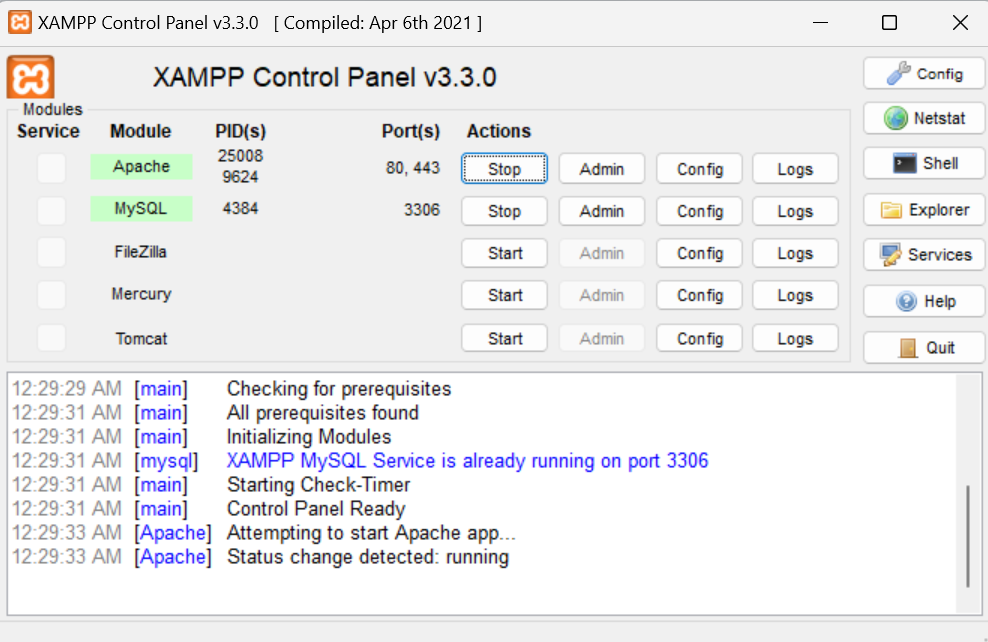
\includegraphics[width=1\textwidth]{img/xamppactivar.png}
    \caption{Pantalla de inicio de XAMPP con las funciones de Apache y MySQL activadas. Fuente propia.}
    \label{fig:xamppactivar}
\end{figure}[h]
Con el objetivo de ilustrar los requisitos funcionales con los que debe cumplir la aplicacion web para su correcto funcionamiento, se presentan una serie de tablas. Los requisitos funcionales descritos en las tablas \ref{RF-01} hasta la \ref{RF-07} han sido obtenidos del TFG \cite{Martos2024}, ya que se mantienen en la versión de la app propuesta en este proyecto. Por otro lado, los requisitos funcionales descritos en las tablas \ref{RF-08} hasta la \ref{RF-11} reflejan los requisitos funcionales nuevos.
\begin{table}[p]
    \centering
    \begin{tabularx}{\linewidth}{ p{0.21\columnwidth} p{0.71\columnwidth} }
        \toprule
        \textbf{RF-01}    & \textbf{Iniciar sesión}\\
        \toprule
        \textbf{Descripción}              & Todos los usuarios deben introducir de forma obligatoria su correo electrónico, tipo de usuario y contraseña para poder acceder a la página web.   \\
        \textbf{Importancia}                & Baja \\
        \bottomrule
    \end{tabularx}
    \caption{RF-01 Iniciar Sesión \cite{Martos2024}}
    \label{RF-01}
\end{table}

\begin{table}[p]
    \centering
    \begin{tabularx}{\linewidth}{ p{0.21\columnwidth} p{0.71\columnwidth} }
        \toprule
        \textbf{RF-02}    & \textbf{Consultar pacientes y usuarios}\\
        \toprule
        \textbf{Descripción}              & Otorgar acceso a la lista completa de usuarios o pacientes, según los permisos asignados al usuario, y permitir la realización de búsquedas específicas dentro de ella.   \\
        \textbf{Importancia}                & Media \\
        \bottomrule
    \end{tabularx}
    \caption{RF-02 Consultar pacientes y usuarios \cite{Martos2024}}
    \label{RF-02}
\end{table}

\begin{table}[p]
    \centering
    \begin{tabularx}{\linewidth}{ p{0.21\columnwidth} p{0.71\columnwidth} }
        \toprule
        \textbf{RF-03}    & \textbf{Gestionar pacientes y usuarios}\\
        \toprule
        \textbf{Descripción}              & Permitir la creación y eliminación de cuentas, así como la modificación de los datos almacenados en las cuentas de pacientes y médicos. La capacidad para realizar estas acciones depende del nivel de acceso que el usuario tenga en el sistema web.   \\
        \textbf{Importancia}                & Media \\
        \bottomrule
    \end{tabularx}
    \caption{RF-03 Gestionar pacientes y usuarios \cite{Martos2024}}
    \label{RF-03}
\end{table}

\begin{table}[p]
    \centering
    \begin{tabularx}{\linewidth}{ p{0.21\columnwidth} p{0.71\columnwidth} }
        \toprule
        \textbf{RF-04}    & \textbf{Realizar actividad}\\
        \toprule
        \textbf{Descripción}              & Ofrece las opciones de iniciar y finalizar actividades, así como la opción de guardar o descartar estas mismas.   \\
        \textbf{Importancia}                & Alta \\
        \bottomrule
    \end{tabularx}
    \caption{RF-04 Realizar actividad \cite{Martos2024}}
    \label{RF-04}
\end{table}

\begin{table}[p]
    \centering
    \begin{tabularx}{\linewidth}{ p{0.21\columnwidth} p{0.71\columnwidth} }
        \toprule
        \textbf{RF-05}    & \textbf{Mostrar actividades}\\
        \toprule
        \textbf{Descripción}              & Presenta al usuario en una lista las actividades realizadas por el paciente, permitiendo diferentes visualizaciones y llevar a cabo filtrados.   \\
        \textbf{Importancia}                & Alta \\
        \bottomrule
    \end{tabularx}
    \caption{RF-05 Mostrar actividades \cite{Martos2024}}
    \label{RF-05}
\end{table}

\begin{table}[p]
    \centering
    \begin{tabularx}{\linewidth}{ p{0.21\columnwidth} p{0.71\columnwidth} }
        \toprule
        \textbf{RF-06}    & \textbf{Consultar estadísticas}\\
        \toprule
        \textbf{Descripción}              & Visualización de los datos relacionados con las actividades realizadas por el paciente, ya sea de una actividad en concreto o de todas en conjunto.   \\
        \textbf{Importancia}                & Media \\
        \bottomrule
    \end{tabularx}
    \caption{RF-06 Consultar Estadísticas \cite{Martos2024}}
    \label{RF-06}
\end{table}

\begin{table}[p]
    \centering
    \begin{tabularx}{\linewidth}{ p{0.21\columnwidth} p{0.71\columnwidth} }
        \toprule
        \textbf{RF-07}    & \textbf{Gestionar cuenta}\\
        \toprule
        \textbf{Descripción}              & Facilitar a los usuarios las tareas de cambio de contraseña y actualización del correo eléctrónico vinculado a su cuenta.  \\
        \textbf{Importancia}                & Baja \\
        \bottomrule
    \end{tabularx}
    \caption{RF-07 Gestionar cuenta \cite{Martos2024}}
    \label{RF-07}
\end{table}

\begin{table}[p]
    \centering
    \begin{tabularx}{\linewidth}{ p{0.21\columnwidth} p{0.71\columnwidth} }
        \toprule
        \textbf{RF-08}    & \textbf{Personalizar el funcionamiento del dispositivo}\\
        \toprule
        \textbf{Descripción}              & Facilitar al usuario la realización de una prueba que permita personalizar el número de segundos que el script de Arduino identifica como congelamiento de la marcha.  \\
        \textbf{Importancia}                & Media \\
        \bottomrule
    \end{tabularx}
    \caption{RF-08 Personalizar el funcionamiento del dispositivo. Fuente propia}
    \label{RF-08}
\end{table}

\begin{table}[p]
    \centering
    \begin{tabularx}{\linewidth}{ p{0.21\columnwidth} p{0.71\columnwidth} }
        \toprule
        \textbf{RF-09}    & \textbf{Almacenar datos diarios}\\
        \toprule
        \textbf{Descripción}              & Facilitar a los usuarios de tipo 'paciente' la posibilidad de rellenar 2 formularios correspondientes a un diario de tomas de medicación y un diario de fluctuaciones motoras.  \\
        \textbf{Importancia}                & Media \\
        \bottomrule
    \end{tabularx}
    \caption{RF-09 Almacenar datos diarios. Fuente propia.}
    \label{RF-09}
\end{table}

\begin{table}[p]
    \centering
    \begin{tabularx}{\linewidth}{ p{0.21\columnwidth} p{0.71\columnwidth} }
        \toprule
        \textbf{RF-10}    & \textbf{Visualización de gráficas}\\
        \toprule
        \textbf{Descripción}              & Facilitar a los usuarios el acceso a una serie de gráficas creadas a partir de los datos almacenados sobre las actividades realizadas y los datos diarios.  \\
        \textbf{Importancia}                & Media \\
        \bottomrule
    \end{tabularx}
    \caption{RF-10 Visualización de gráficas. Fuente propia.}
    \label{RF-10}
\end{table}

\begin{table}[p]
    \centering
    \begin{tabularx}{\linewidth}{ p{0.21\columnwidth} p{0.71\columnwidth} }
        \toprule
        \textbf{RF-11}    & \textbf{Descarga de informe}\\
        \toprule
        \textbf{Descripción}              & Facilitar a los usuariosde tipo 'profesional' la descarga de un informe en PDF conteniendo información relevante sobre el paciente, sus actividades realizadas y de forma opcional las gráficas.  \\
        \textbf{Importancia}                & Baja \\
        \bottomrule
    \end{tabularx}
    \caption{RF-11 Visualización de gráficas. Fuente propia.}
    \label{RF-11}
\end{table}
\subsection{Requisitos hardware}
Para asegurar el correcto funcionamiento del dispositivo es necesario que el cinturón y la tobillera contengan un circuito configurado de forma correcta, tal como se indica en el Anexo E, mediante la figura \ref{fig:esquemahardware}, y conteniendo los siguientes componentes:
\begin{itemize}
    \item Microcontrolador Arduino UNO3, conectado a un Arduino proto shield que posibilita la conexión de múltiples cables a cada pin de la placa Arduino UNO.
    \item Fuente de alimentación recargable 9V, conectada a la placa mediante un cable adaptador de bateria Arduino DC 9V.
    \item Interruptor ON/OFF.
    \item 2 pulsadores 'start' y 'stop'
    \item Módulo bluetooth HC-05, necesario para la comunicación bidireccional con el servidor web.
    \item Pantalla de display LCD 16x2 con Interfaz I2C 2x16 incorporada, la cual facilita una conexión más sencilla, utilizando tan solo 4 cables.
    \item Sensor acelerómetro y giroscopio MPU-6050.
    \item Cable multihilo, conectado a los cables provenientes de la placa mediante un conector macho-hembra.
    \item Cables de calibre 28 AWG (en total unos 3m) para la conexión de los diferentes componentes a la placa Arduino.
\end{itemize}
\section{Instalación / Puesta en marcha}
\subsection{Puesta en marcha del dispositivo Arduino}
\begin{enumerate}
    \item Calibración del dispositivo: El primer paso para asegurar un correcto funcionamiento del dispositivo es calibrar el sensor MPU-6050 mediante el script de calibración 'calibracionDMP.ino'. Para ello se conectará por cable la placa Arduino UNO del dispositivo con el ordenador en que tengamos este script. Utilizando la aplicación Arduino IDE cargamos el script en la placa, tal como muestra la figura \ref{fig:cargascript}.
    \begin{figure}[h]
        \centering
        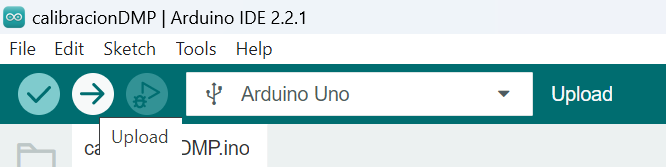
\includegraphics[width=1\textwidth]{img/cargascript.png}
        \caption{Carga del script 'calibracionDMP.ino' utilizando Arduinio IDE. Fuente propia.}
        \label{fig:cargascript}
    \end{figure}
    Tras la carga del script, manteniendo la conexión por cable con la placa, es necesario abrir la función 'Serial Monitor' de Arduino IDE, en la cual observaremos la comunicación serial con el dispositivo Arduino. Será necesario enviar un carácter cualquiera para iniciar el proceso de calibración, y al finalizar el proceso obtendremos unos resultados \ref{fig:calibracion}.
    \begin{figure}[h]
        \centering
        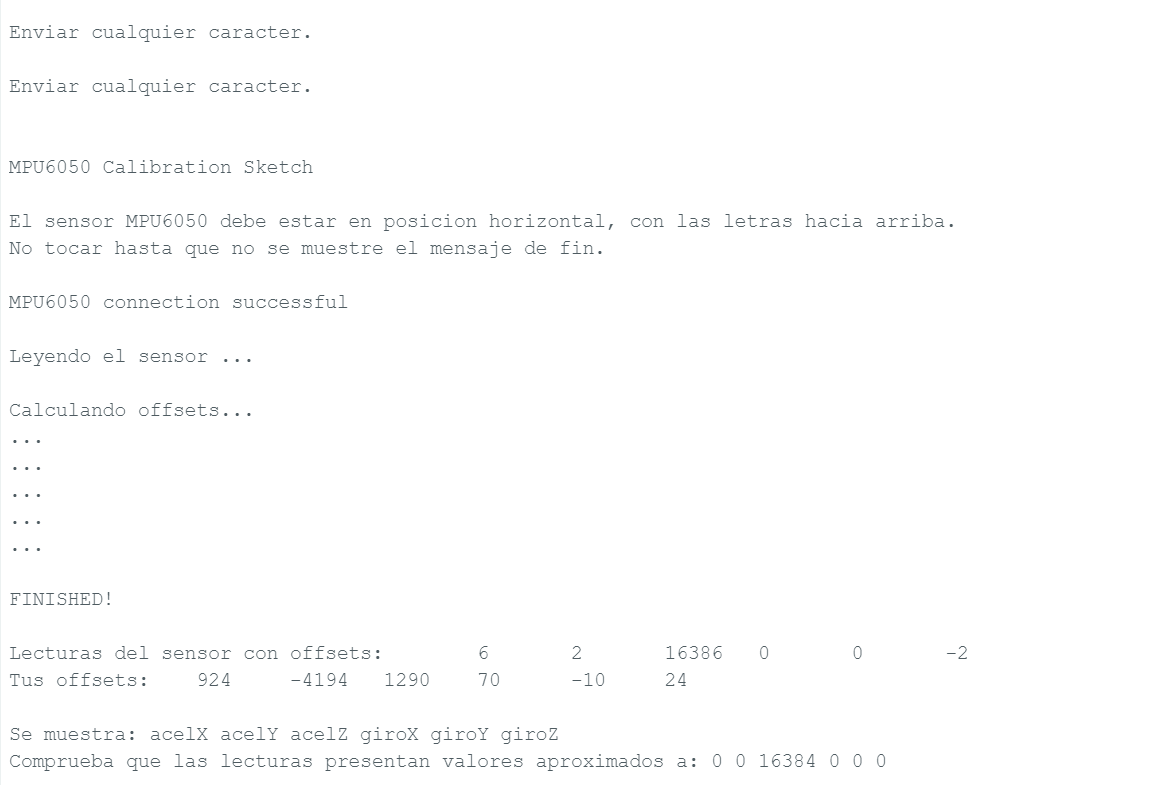
\includegraphics[width=1\textwidth]{img/calibracion.png}
        \caption{Monitor serial de Arduino IDE durante una calibración exitosa. Fuente propia.}
        \label{fig:calibracion}
    \end{figure}
    \item Carga del script: Tras haber calibrado exitosamente el sensor MPU-6050, se debe sustituir el script de calibración por el script general (en este caso la versión 5 que tiene como título laser), que contiene el programa para el funcionamiento del dispositivo. Teniendo la placa conectada por cable cargaremos el script y posteriormente podremos desconectar el cable. El dispositivo está listo para funcionar.
\end{enumerate}
\subsection{Instalación y puesta en marcha de la aplicación web}
\begin{enumerate}
    \item Tras asegurarnos de que en el ordenador a utilizar se cumplen los requisitos software previamente mencionados (instalación de la apicación XAMPP y de Visual Studio Code, alojamiento de la carpeta con archivos de código en xampp/htdocs, instalación de Node.js y ejecución de las funciones Apache y MySQL de XAMPP) deberíamos ser capaces de acceder a la app insertando el link en cualquier navegador del dispositivo:
    
    \url{http://localhost/Web_VisualStudio/common/login.html} 
    \item Para utilizar las funciones de la app que implican conexión en tiempo real con el dispositivo (realización de actividades y prueba de personalización), debemos seguir unos pasos adicionales:
    \begin{itemize}
        \item Conectar el dispositivo, con nombre 'TFG1', al ordenador (para cambiar la configuración del módulo bluetooth y mostrarse con otro nombre u contraseña se puede conectar el pin enable, que normalmente queda libre, al pin 5V de la placa Arduino y utilizar un script de Arduino para ello)
        \item Abrir la carpeta de archivos de código en Visual Studio Code y ejecutar el comando 'node server.js' en la terminal integrada de la carpeta ArduinoServer. De esta forma pondremos en marcha el servidor. En la figura \ref{fig:servidor} observamos una activación exitosa del servidor.
            \begin{figure}[h]
                \centering
                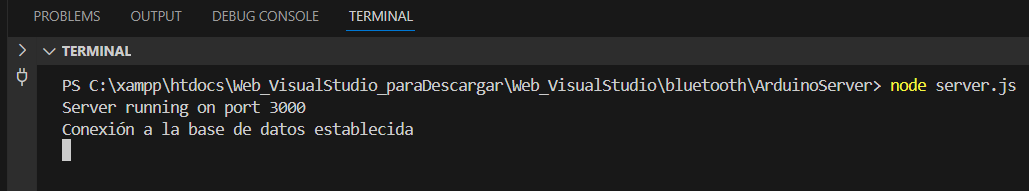
\includegraphics[width=1\textwidth]{img/servidor.png}
                \caption{Activación del servidor exitosa. Fuente propia.}
                \label{fig:servidor}
            \end{figure}
        \item Ejecutar el archivo 'bridge.py', ajustando el puerto serial según el puerto al que esté conectado el dispositivo bluetooth \ref{fig:bridgepy}. Usualmente este puerto es 'COM3' o 'COM4', pero podemos cocnsultar qué puerto se está utilizando en el administrador de dispositivos \ref{fig:admintareas}, pulsando en los puertos bluetooth y consultando en el apartado 'eventos' la conexión de dispositivos a los mismos. Tras ajustar el puerto, al ejecutar el archivo deberíamos recibir en la terminal algo similar a lo mostrado en la figura \ref{fig:bridgeejecutando} de forma continuada. En caso de observar algo distinto, es indicación de que el servidor no funciona correctamente (habría que repetir el paso anterior) o de que el puerto especificado no es el correcto.
            \begin{figure}[h]
                \centering
                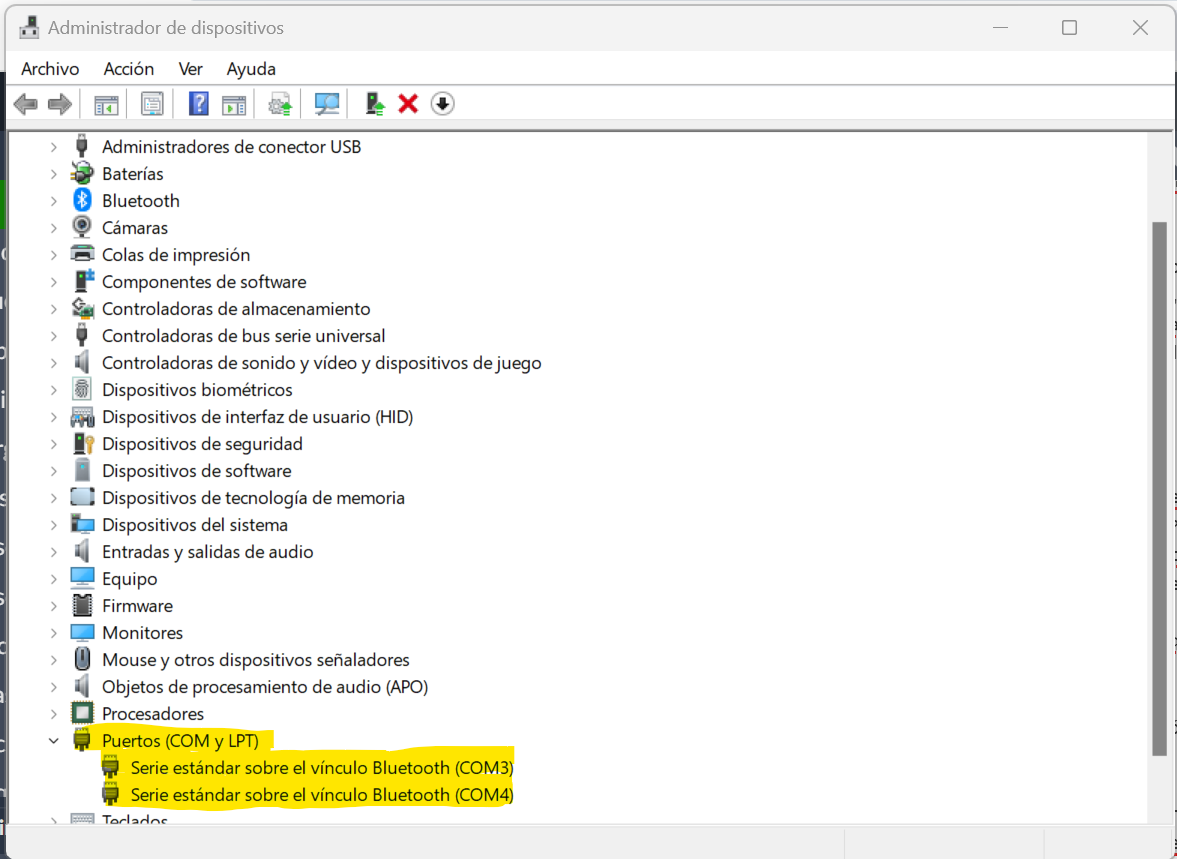
\includegraphics[width=1\textwidth]{img/admindispositivos.png}
                \caption{Consulta en el administrador de dispositivos. Fuente propia.}
                \label{fig:admintareas}
            \end{figure}
            \begin{figure}[h]
                \centering
                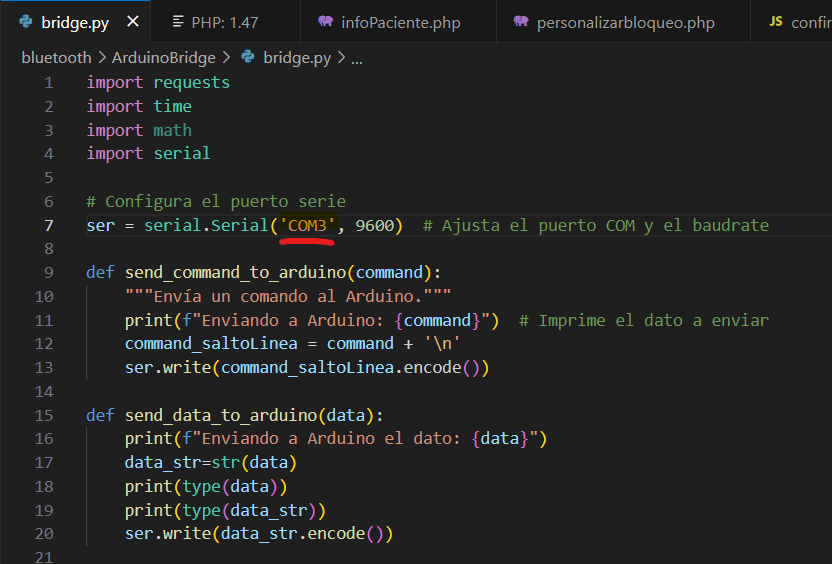
\includegraphics[width=1\textwidth]{img/bridgepy.png}
                \caption{Archivo bridge.py en que se especifica el puerto serial al que está conectado el dispositivo. Fuente propia.}
                \label{fig:bridgepy}
            \end{figure}
            \begin{figure}[h]
                \centering
                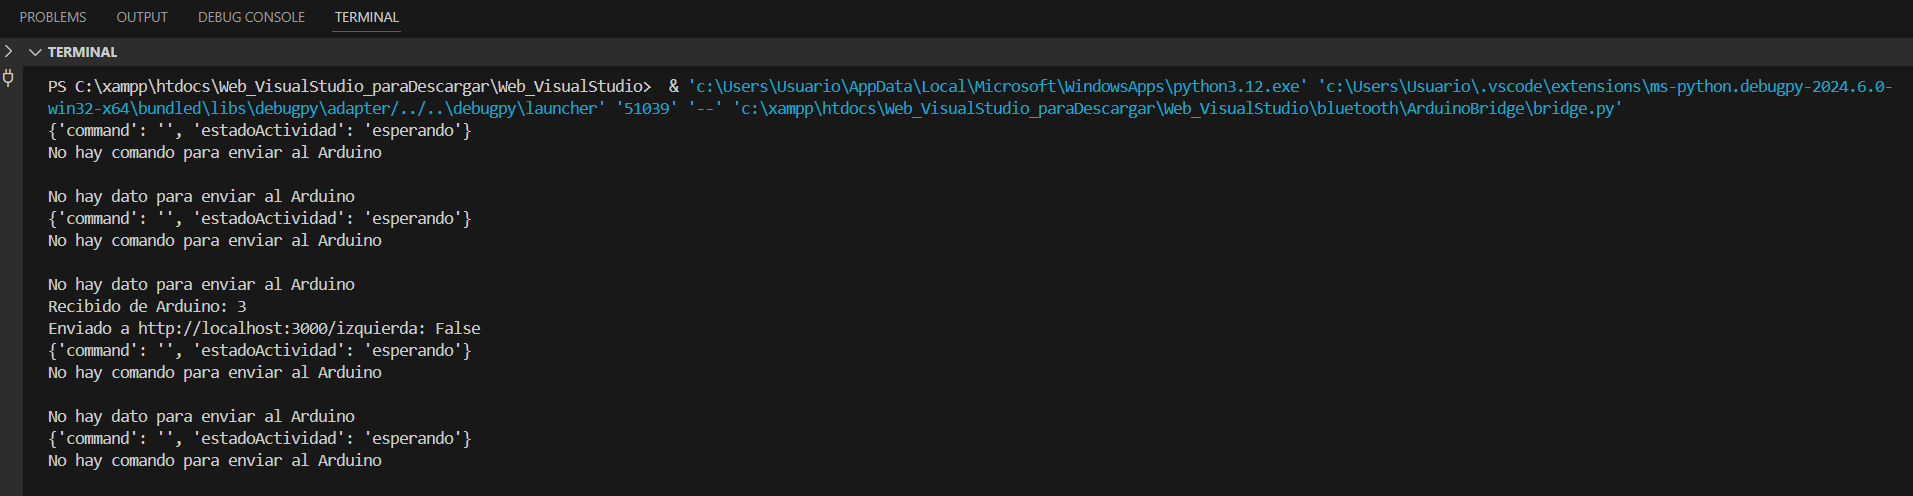
\includegraphics[width=1\textwidth]{img/bridgeejecutando.png}
                \caption{Teminal durante la ejecución exitosa del archivo bridge.py . Fuente propia.}
                \label{fig:bridgeejecutando}
            \end{figure}
    \end{itemize}
\end{enumerate}
\section{Manuales y/o Demostraciones prácticas}
Con el objetivo de clarificar el modo de uso y funcionamiento de las nuevas funciones implementadas en la aplicación web se muestran a continuación unas instrucciones para el uso de la aplicación por parte de los diferentes usuarios, así como unas indicaciones para el acceso a videos de demostración del funcionamiento de estas funciones.
\subsection{Instrucciones para el uso de las nuevas funciones en la aplicación web}
La pantalla de acceso a la aplicación web, en la que observamos un formulario de log-in se muestra en la figura \ref{fig:inicio}. Rellenando el formulario con unas credenciales válidas de un usuario con cuenta registrada en la aplicación obtendremos el acceso a la app con las funciones correspondientes a cada tipo de usuario.
\begin{figure}[h]
    \centering
    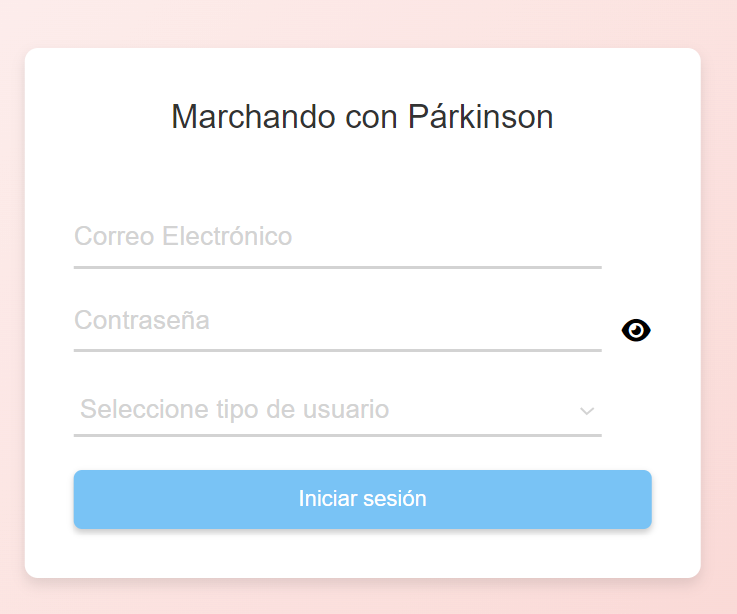
\includegraphics[width=1\textwidth]{img/inicio.png}
    \caption{Inicio de sesión en la aplicación web. Fuente propia.}
    \label{fig:inicio}
\end{figure}
Al iniciar sesión con una cuenta de tipo 'profesional', accederemos a la pantalla de inicio mostrada en la figura \ref{fig:inicioprof}, desde donde tendremos acceso al menú de navegación del profesional, y a la lista de pacientes asignados. 
\begin{figure}[h]
    \centering
    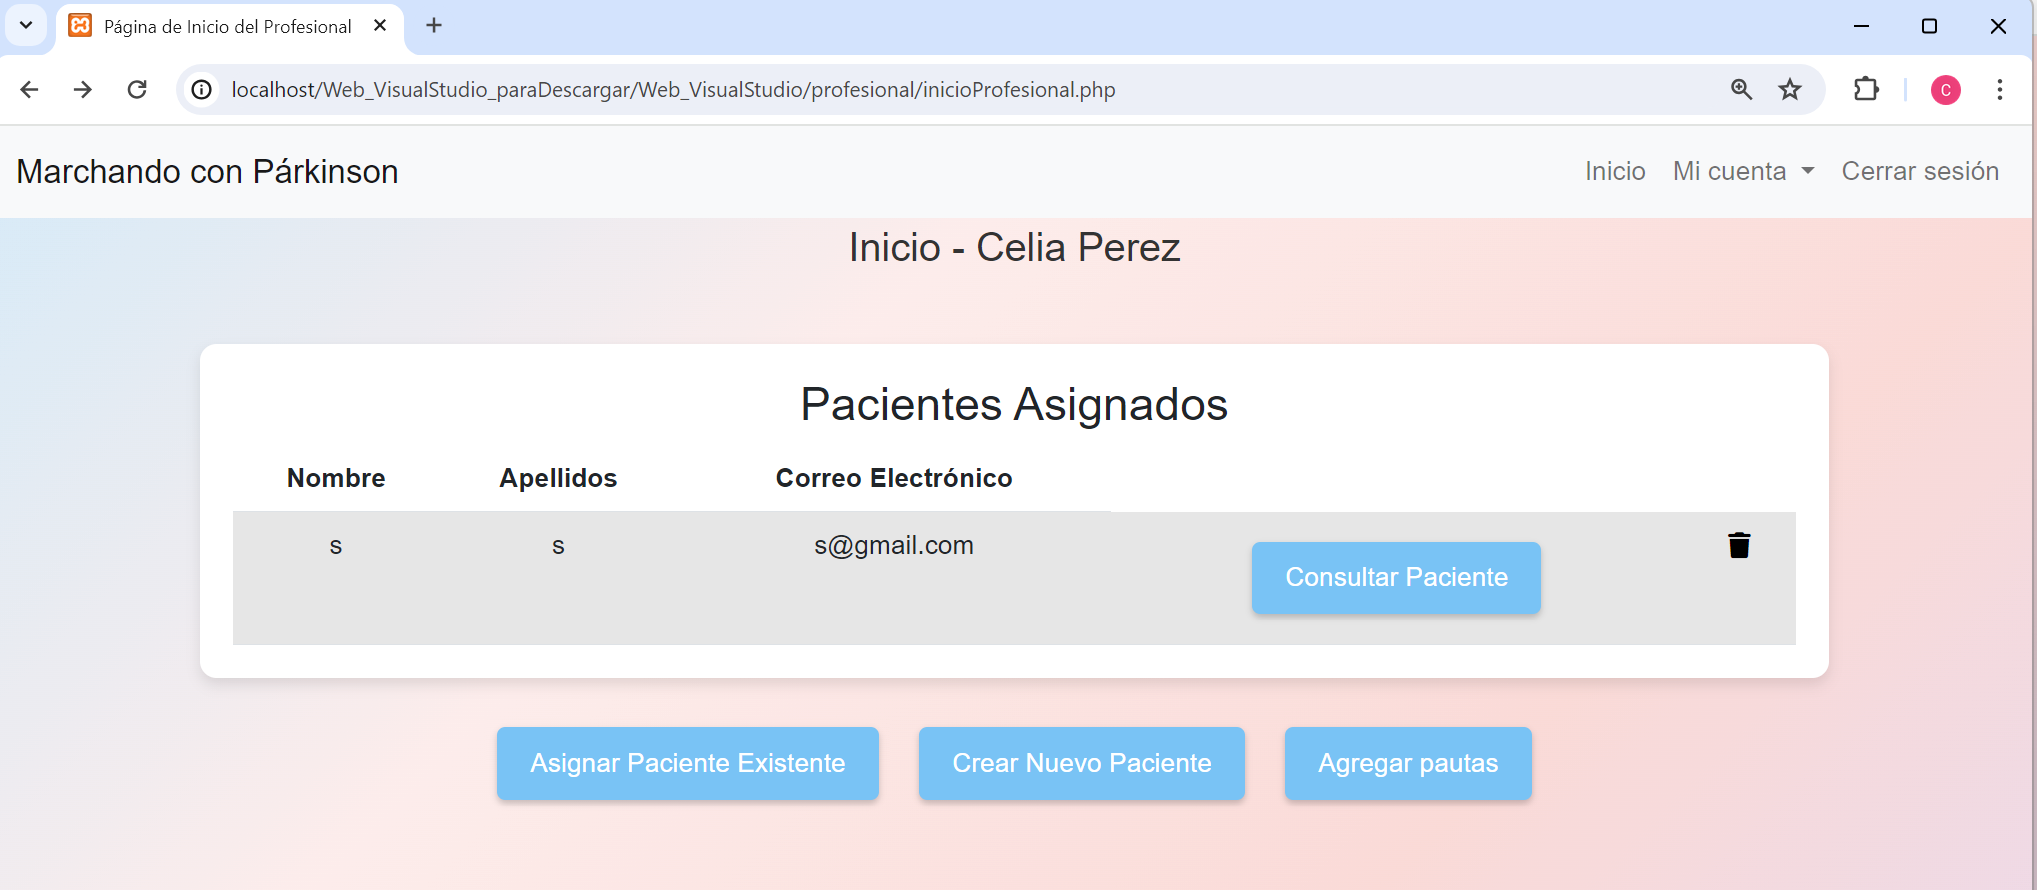
\includegraphics[width=1\textwidth]{img/inicioprof.png}
    \caption{Pantalla de inicio del usuario de tipo 'profesional'. Fuente propia.}
    \label{fig:inicioprof}
\end{figure}

Pulsando en el botón 'Agregar pautas' visualizamos el formulario para agregar una pauta a un paciente \ref{fig:pautasprof}. Para ello debemo seleccionar el ID del paciente a guardar, el número de medicaciones diferentes relacionadas con los síntomas motores del párkinson que el paciente toma cada día y rellenar los datos correspondientes a cada una de esas medicaciones (número de tomas y nombre). Estos datos aparecerán de forma predeterminada como respuestas en el diario de tomas de medicaciones del paciente.

\begin{figure}[h]
    \centering
    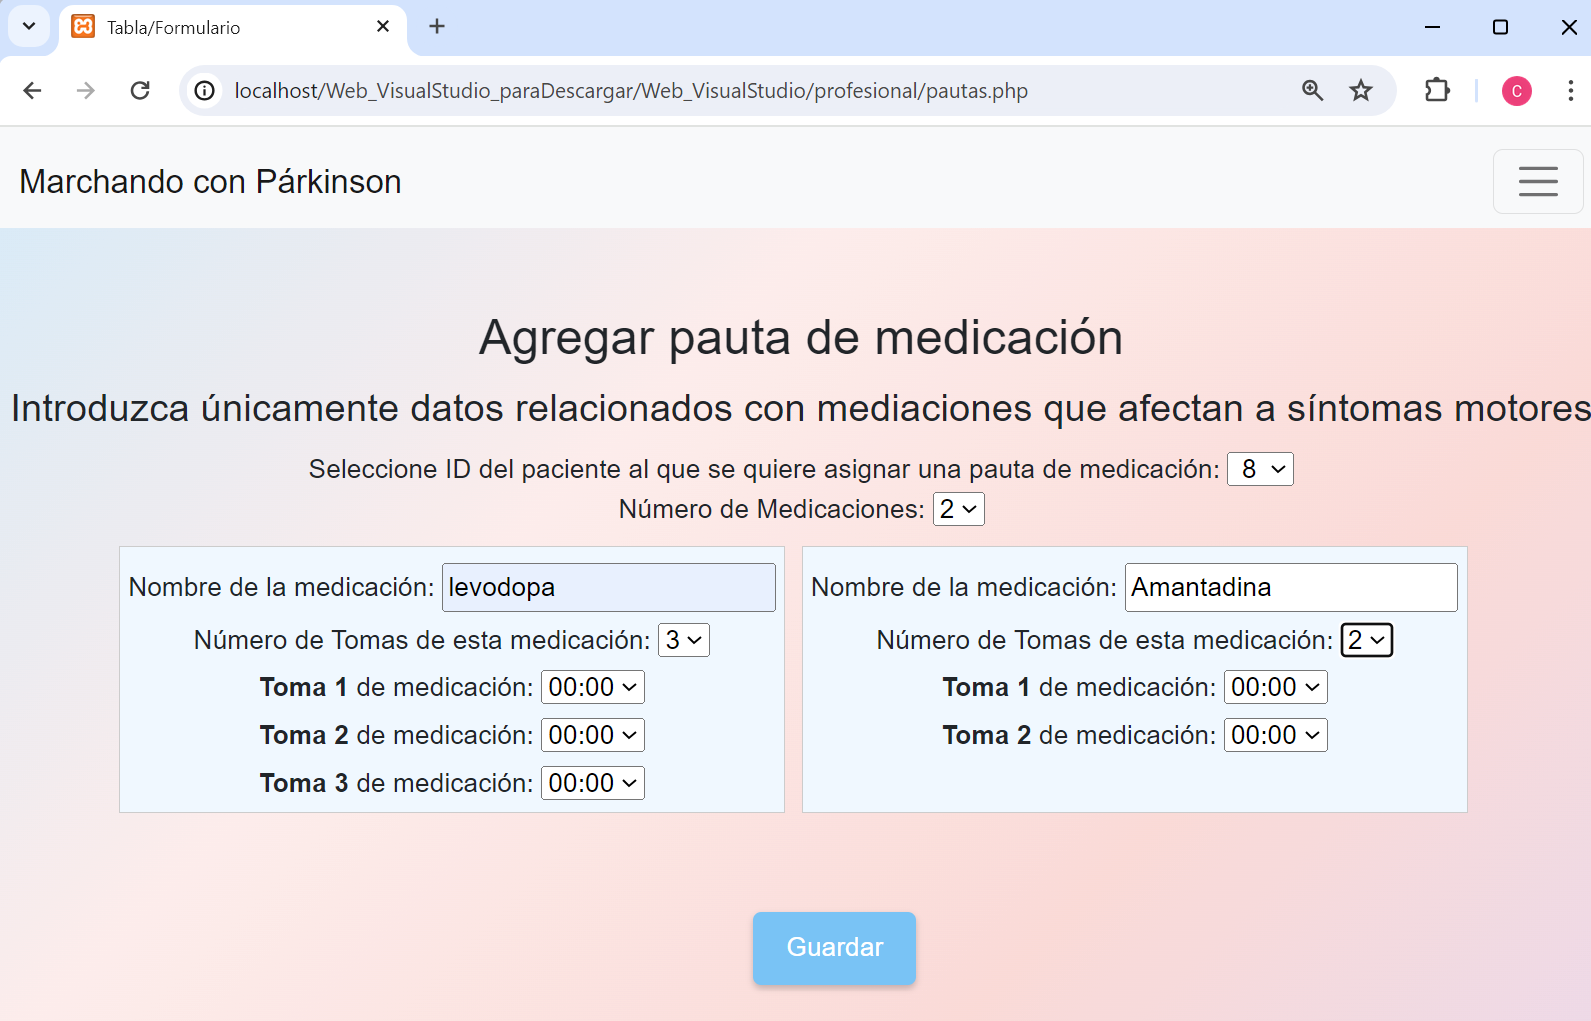
\includegraphics[width=1\textwidth]{img/pautasprof.png}
    \caption{Formulario de asignación de una pauta de medicación a un paciente por parte del profesional. Fuente propia.}
    \label{fig:pautasprof}
\end{figure}
Desde la pantalla de inicio de tipo 'profesional' también podemos consultar los datos almacenados para los pacientes asignados al usuario, desde la pantalla \ref{fig:profverpaciente}. Desde aquí podemos acceder a la prueba de personalización, cuyo funcionamiento se detalla en los videos de demostración y a las actividades y estadísticas del paciente. 

\begin{figure}[h]
    \centering
    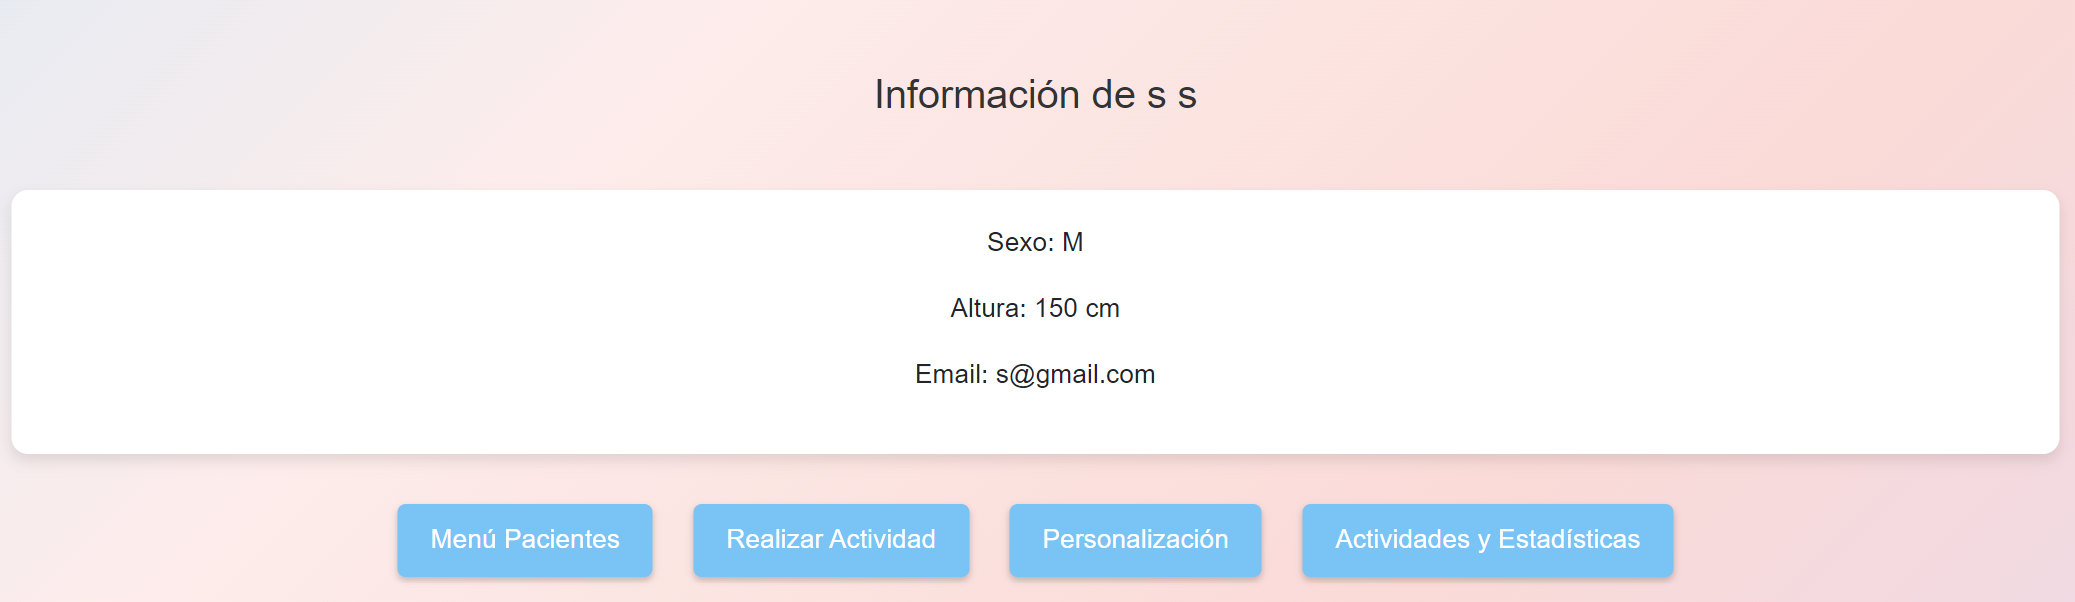
\includegraphics[width=1\textwidth]{img/profverpaciente.png}
    \caption{Consulta de un paciente asignado por parte del profesional. Fuente propia.}
    \label{fig:profverpaciente}
\end{figure}

La prueba de personalización tiene como objetivo guardar durante el comienzo del uso del dispositivo por parte del paciente un número de segundos personalizado a partir de los cuales se detectará un congelamiento de la marcha. Esto se realizará a partir de los segundos que tarde el usuario en dar 1 paso. La prueba se realizará con ayuda del profesional para asegurar su validez, por lo que se encuentra dentro de las funciones del usuario 'profesional'.

Desde el apartado de 'Actividades y Estadísticas' \ref{fig:profestadisticas}, el profesional puede descargar un informe en pdf sobre los datos de las actividades y de forma opcional las gráficas \ref{fig:pdf} o consultar de forma directa las gráficas \ref{fig:graficas}. Para observar los diferentes tipos de gráficas que pueden observarse en este apartado consultar los vídeos de demostraciones.

\begin{figure}[h]
    \centering
    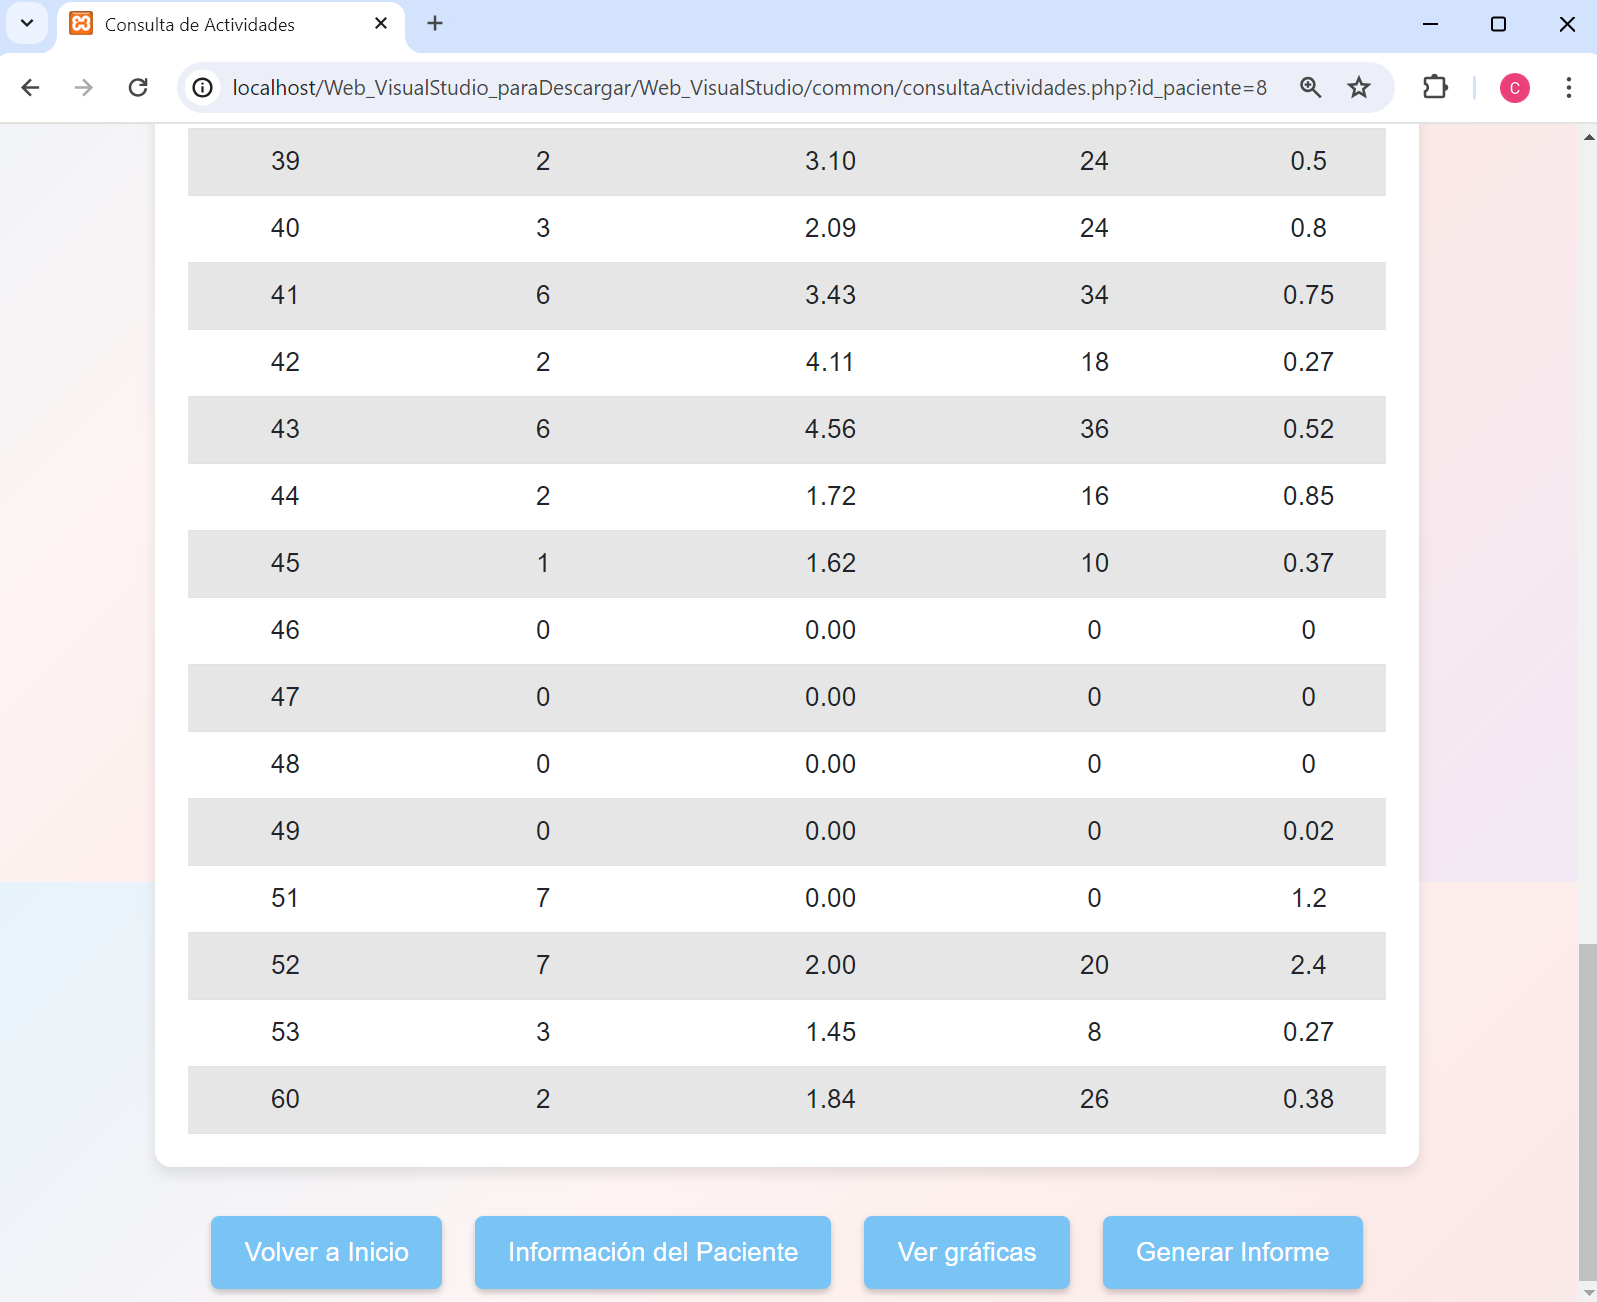
\includegraphics[width=1\textwidth]{img/profestadisticas.png}
    \caption{Vista desde el usuario 'profesional' al apartado de actividades y estadísticas de un paciente asignado. Fuente propia.}
    \label{fig:profestadisticas}
\end{figure}


\begin{figure}[h]
    \centering
    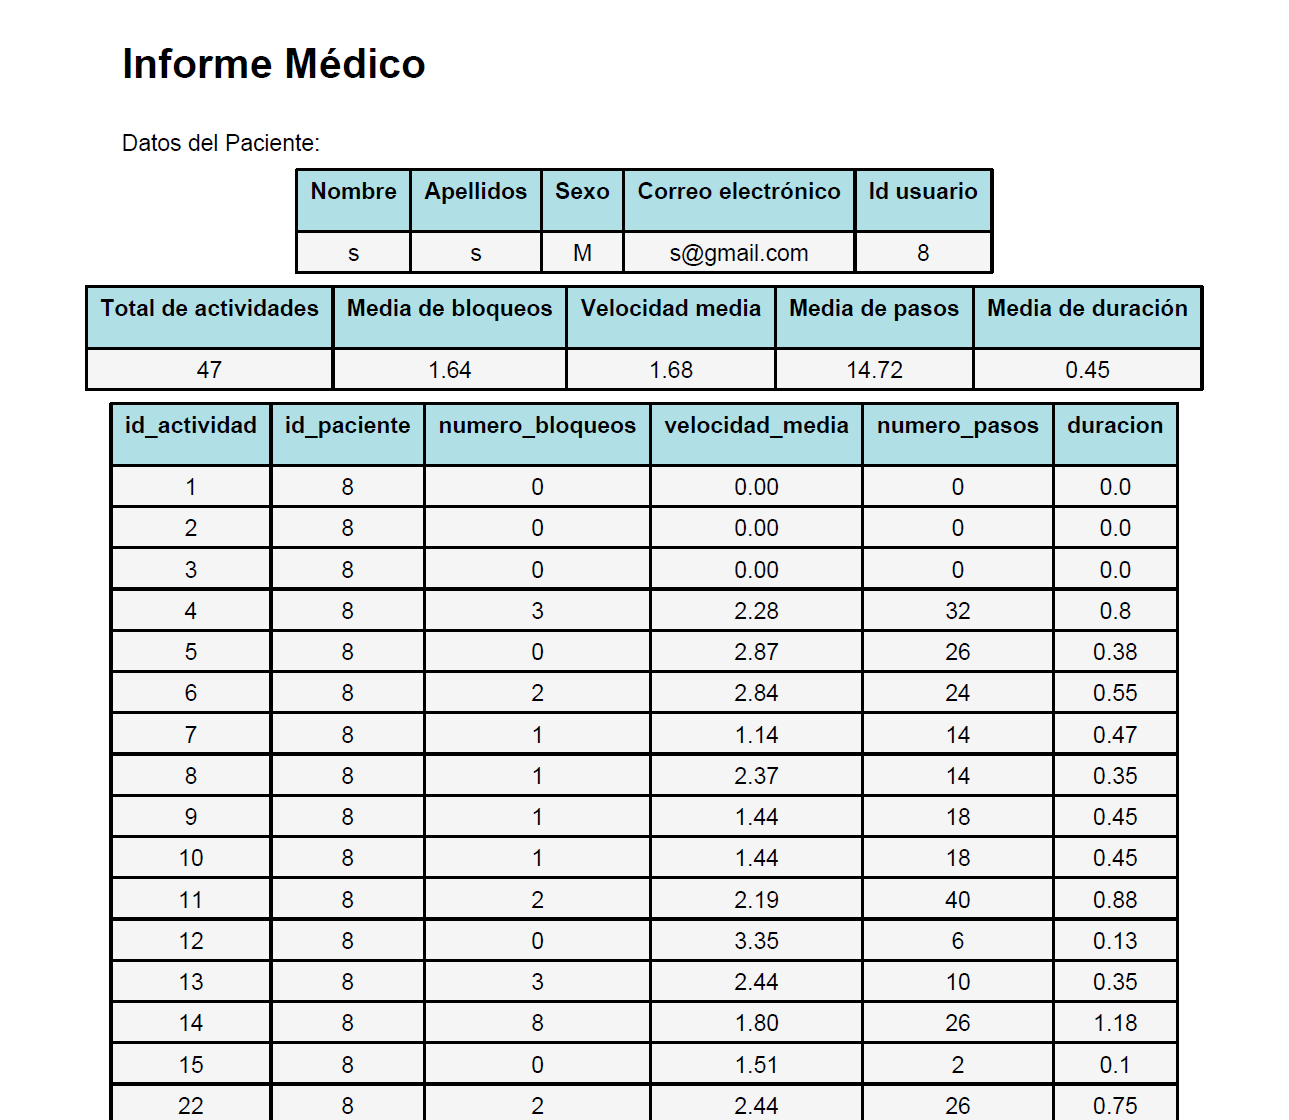
\includegraphics[width=1\textwidth]{img/pdf.png}
    \caption{Pdf generado automáticamente con los datos del paciente. Fuente propia.}
    \label{fig:pdf}
\end{figure}

\begin{figure}[h]
    \centering
    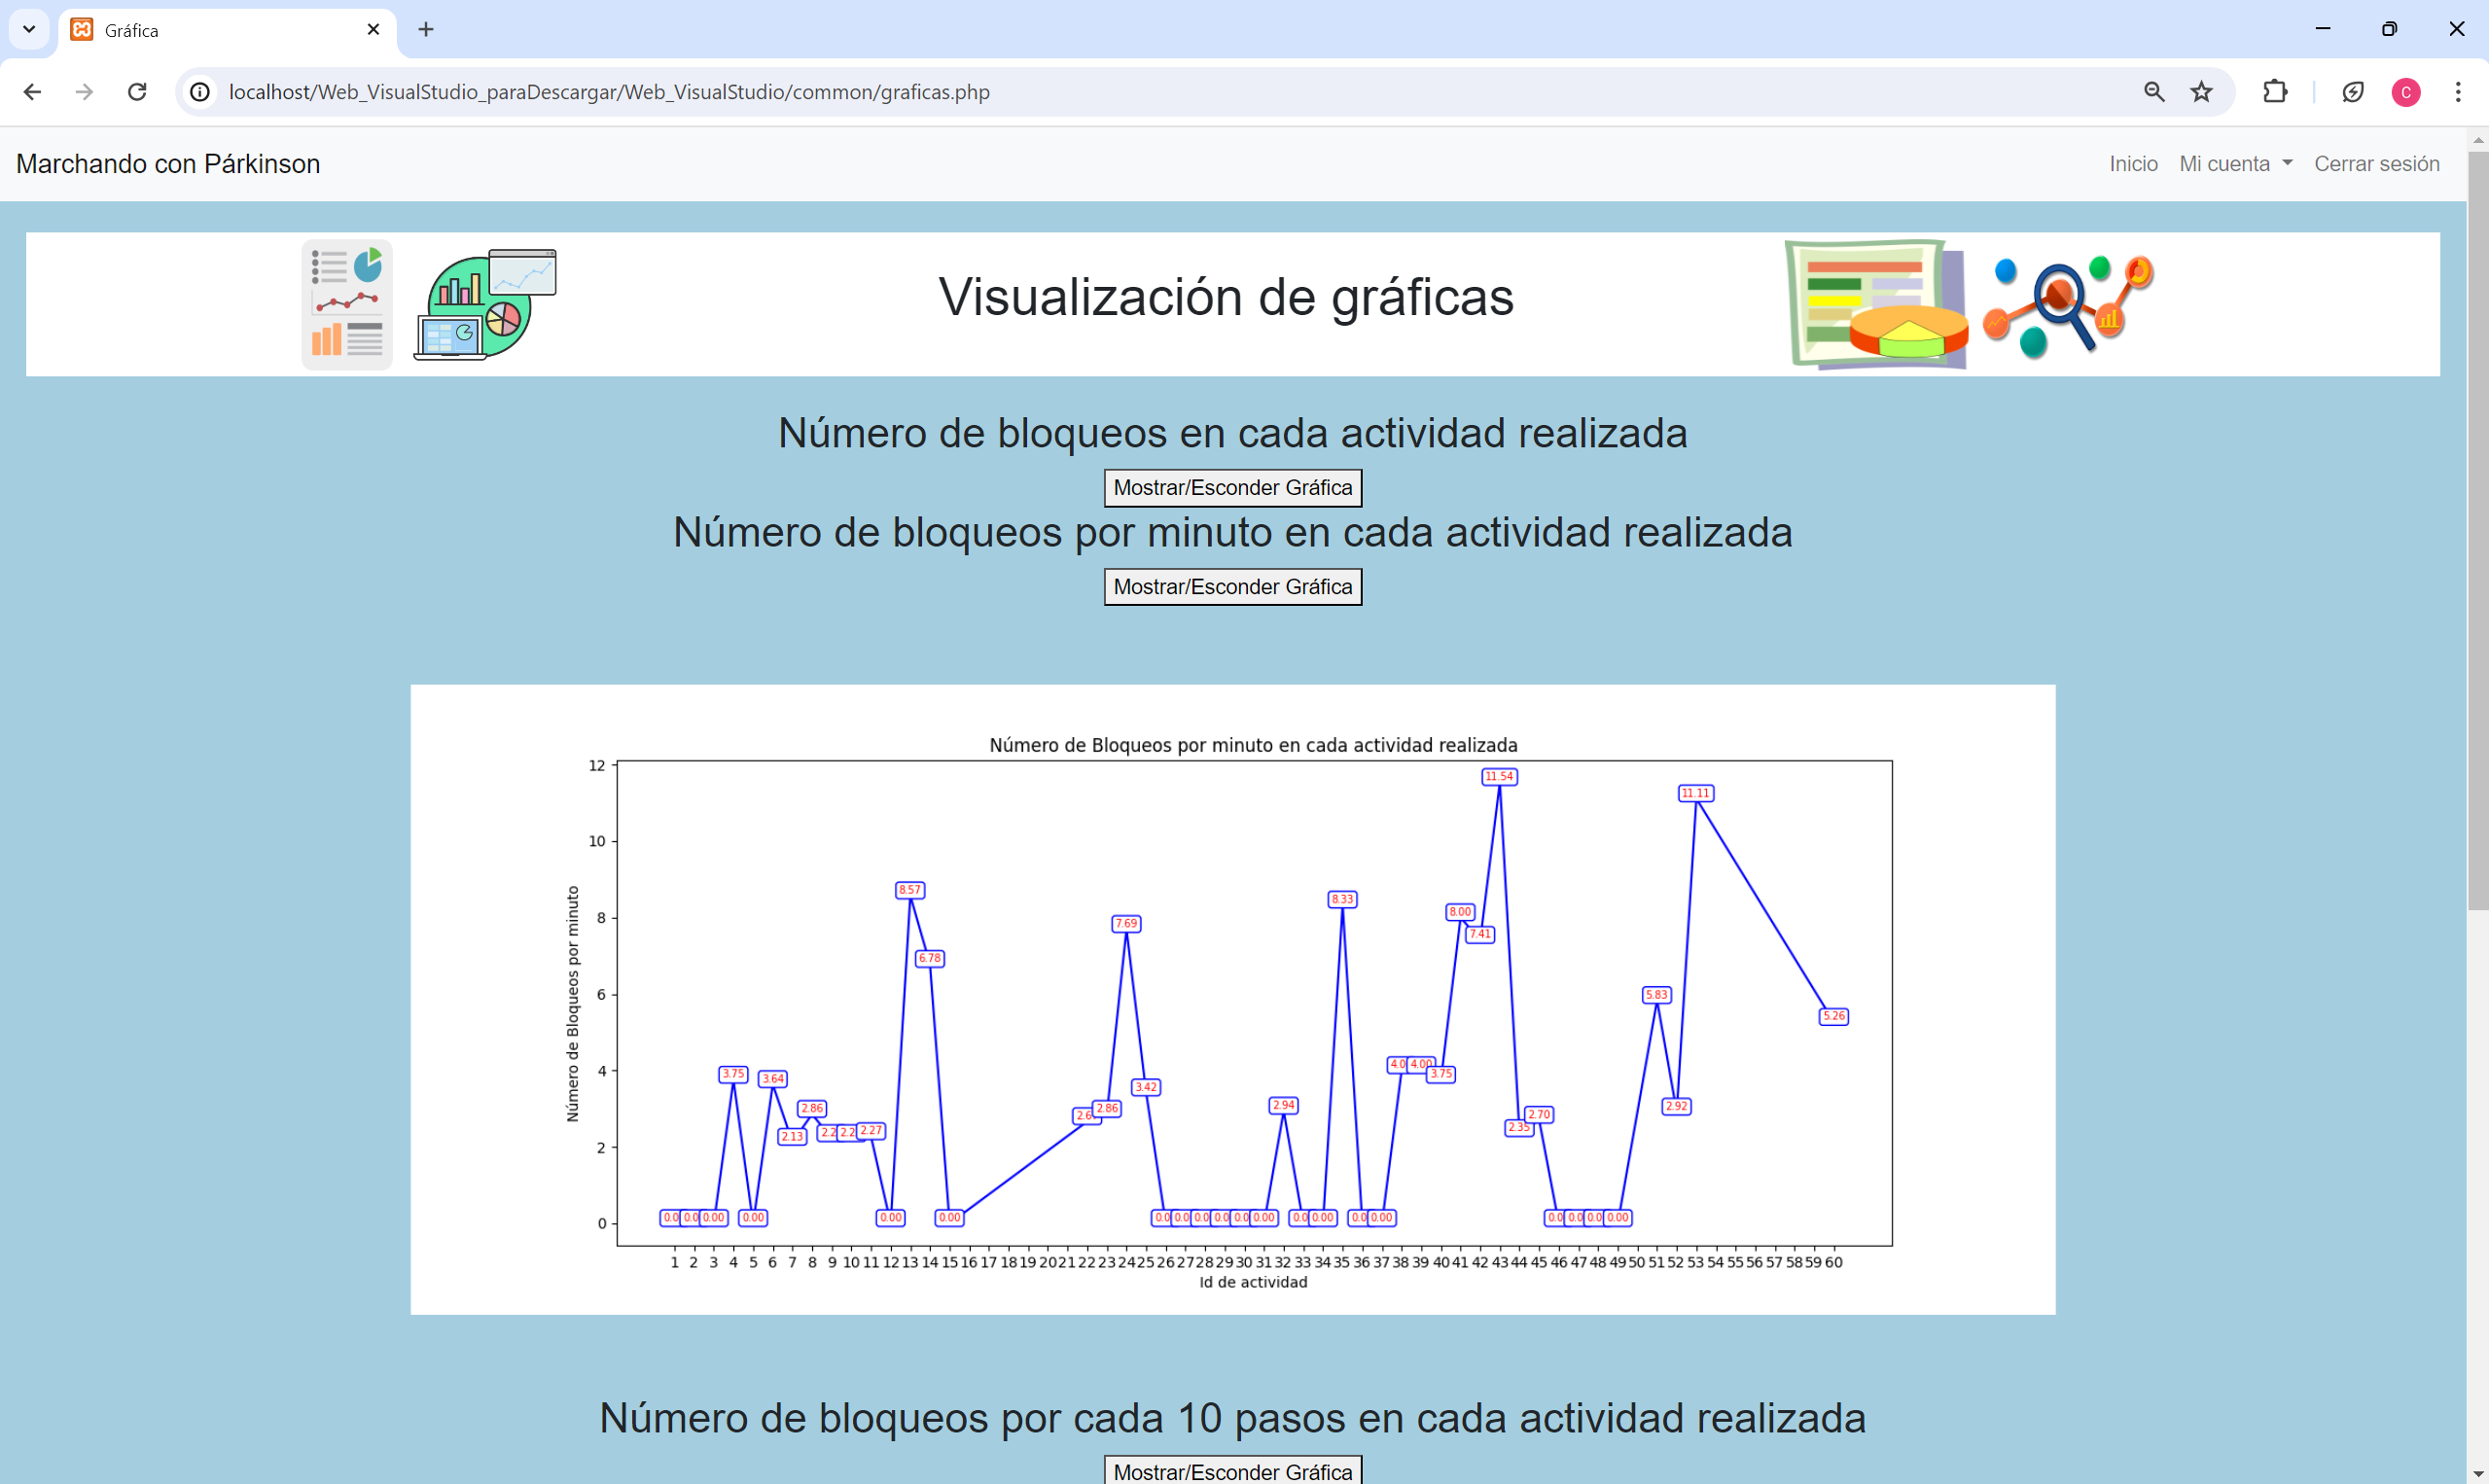
\includegraphics[width=1\textwidth]{img/graficas.png}
    \caption{Vista de las gráficas. Fuente propia.}
    \label{fig:graficas}
\end{figure}

Al acceder a la aplicación con una cuenta de tipo 'paciente', observamos la pantalla mostrada en la figura \ref{fig:iniciopaciente}. En la barra de navegación, observamos un botón 'Acceder al diario', que nos lleva a la pantalla mostrada en la figura \ref{fig:diarios}, a partir de la cual se puede acceder al diario de fluctuaciones (un diario de Hauser, tal como se describe en la memoria de este proyecto) \ref{fig:diariofluc} y al diario de tomas de medicaciones \ref{fig:diariotomas}. En este último diario observaremos como respuestas predeterminadas las correspondientes a la pauta de medicación asignada, en caso de que el profesional encargado la haya insertado como se indicó anteriormente.

\begin{figure}[h]
    \centering
    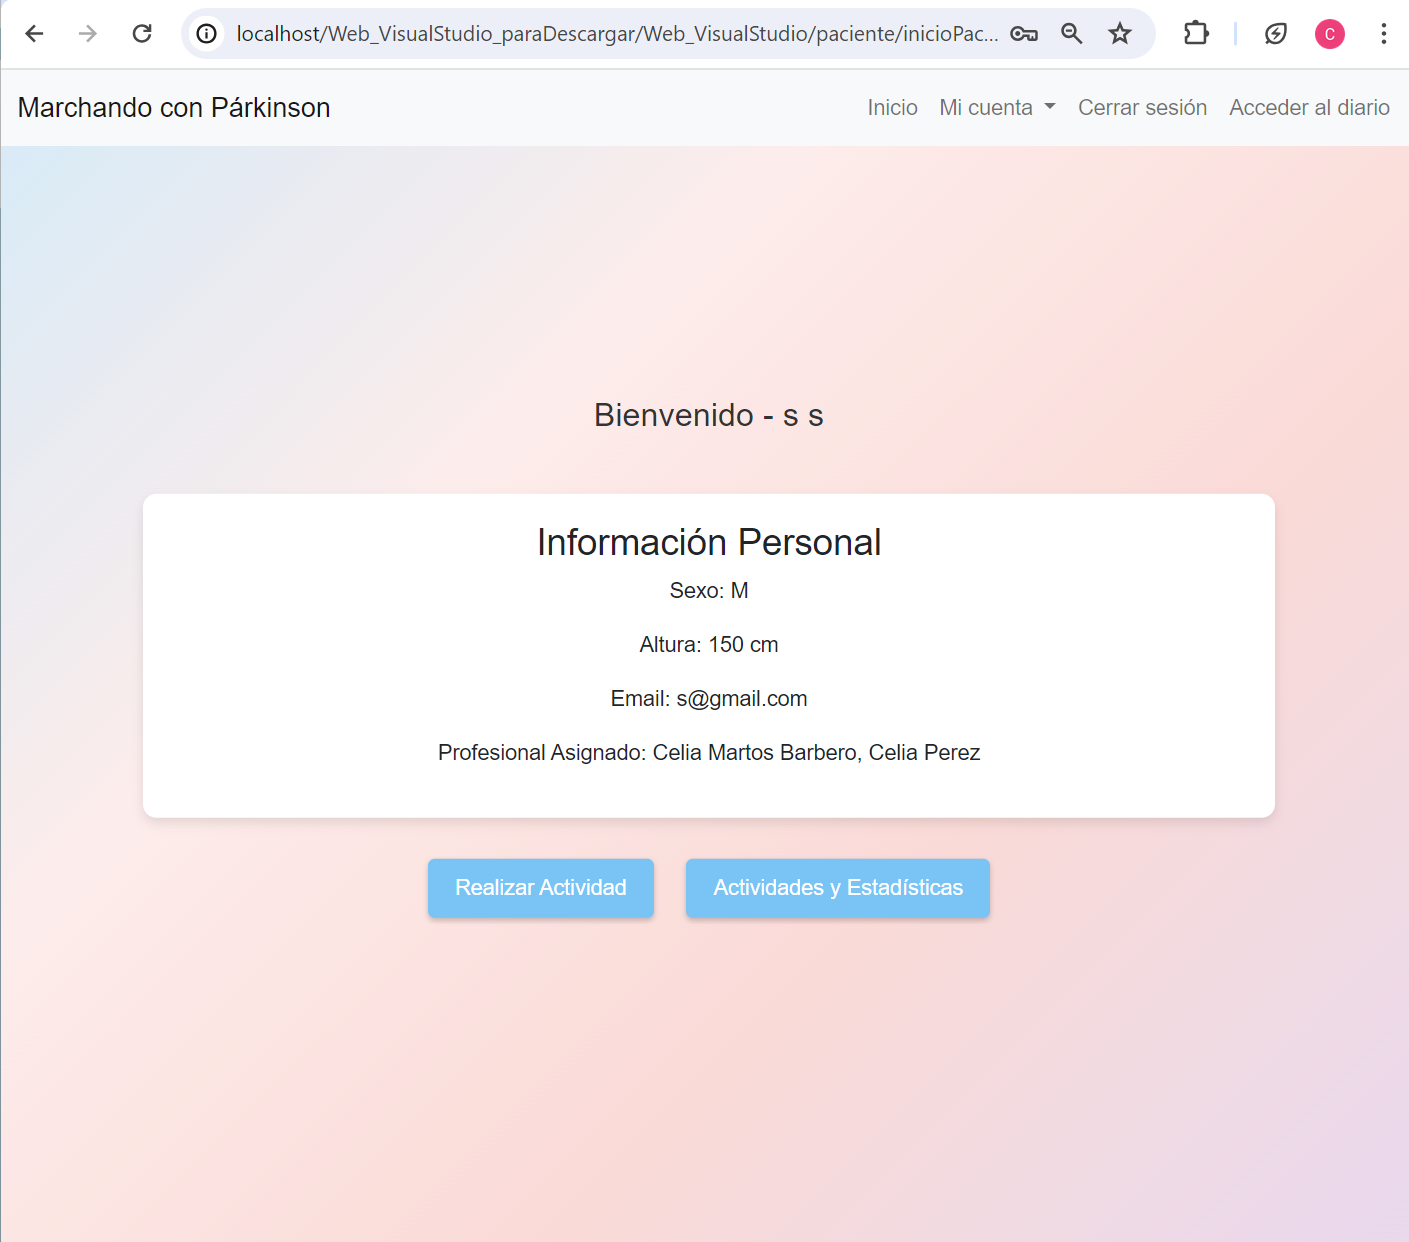
\includegraphics[width=1\textwidth]{img/iniciopaciente.png}
    \caption{Pantalla de inicio del usuario de tipo 'paciente'. Fuente propia.}
    \label{fig:iniciopaciente}
\end{figure}

\begin{figure}[h]
    \centering
    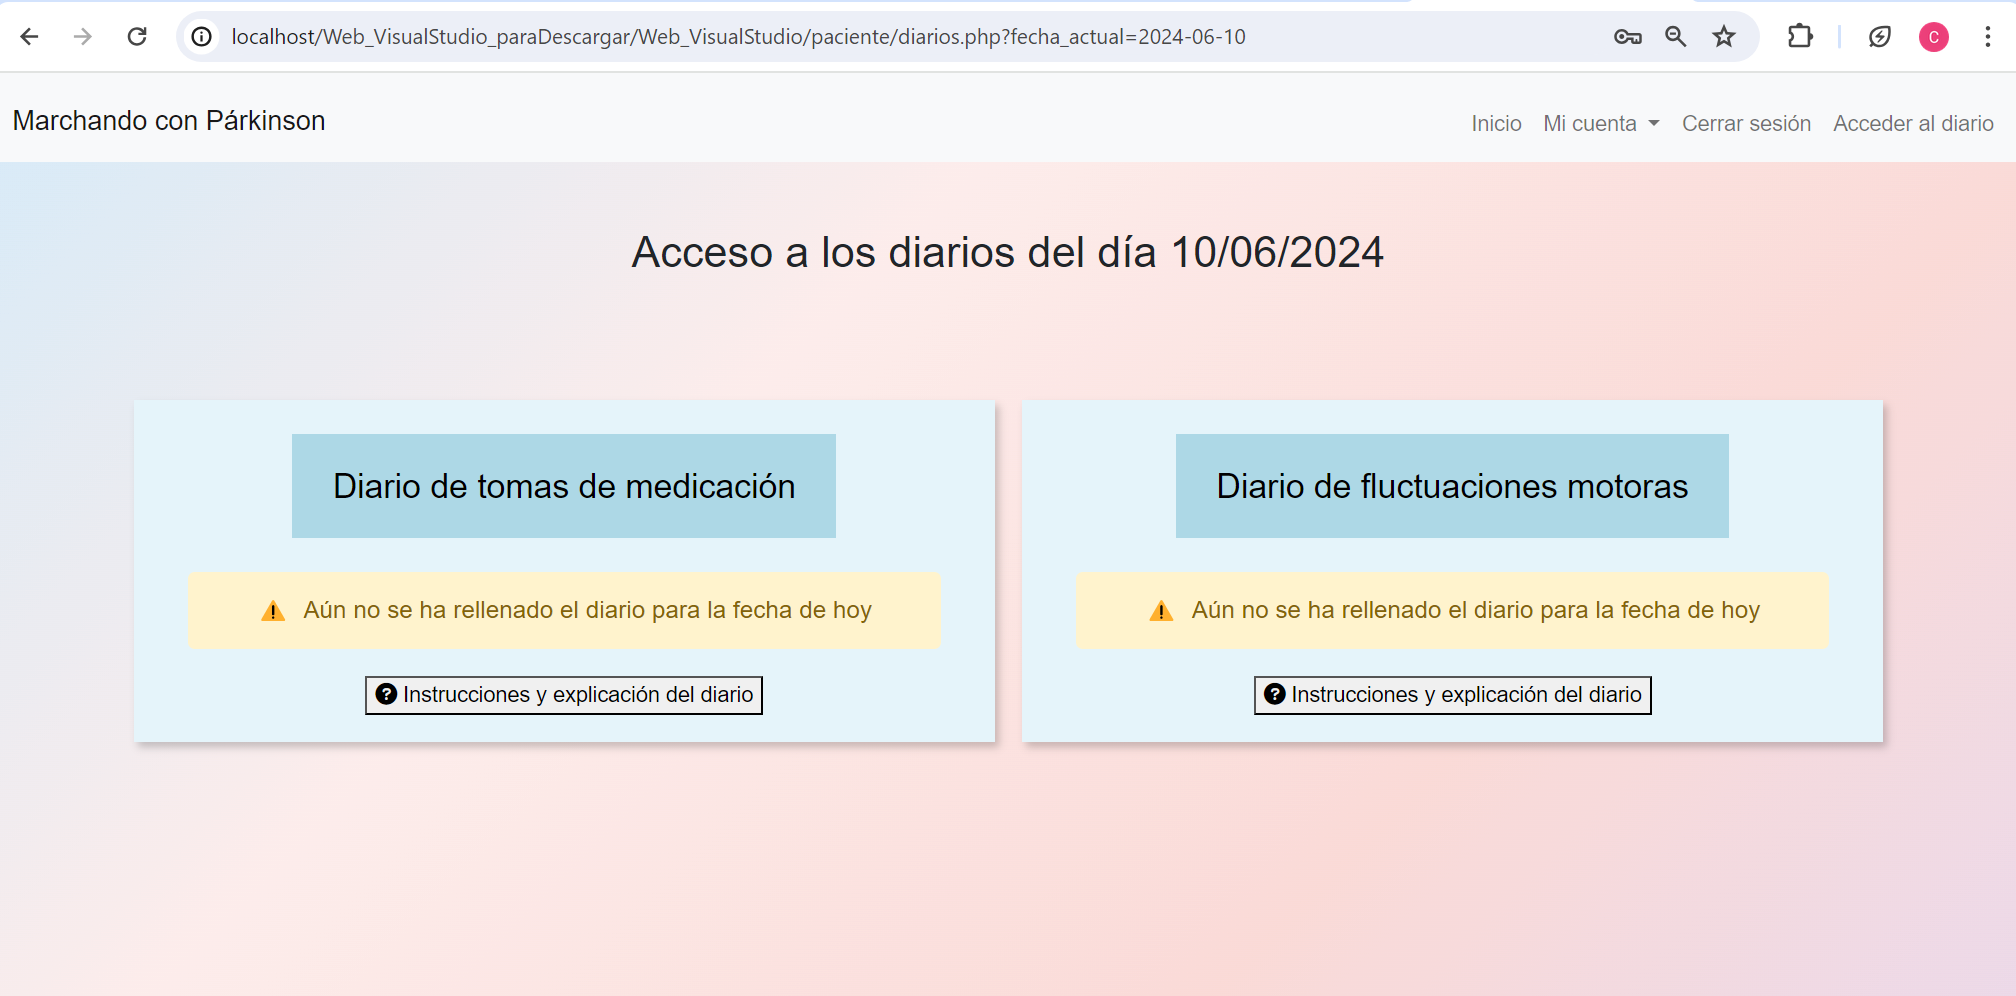
\includegraphics[width=1\textwidth]{img/diarios.png}
    \caption{Pantalla de acceso a los diarios del paciente. Fuente propia.}
    \label{fig:diarios}
\end{figure}

\begin{figure}[h]
    \centering
    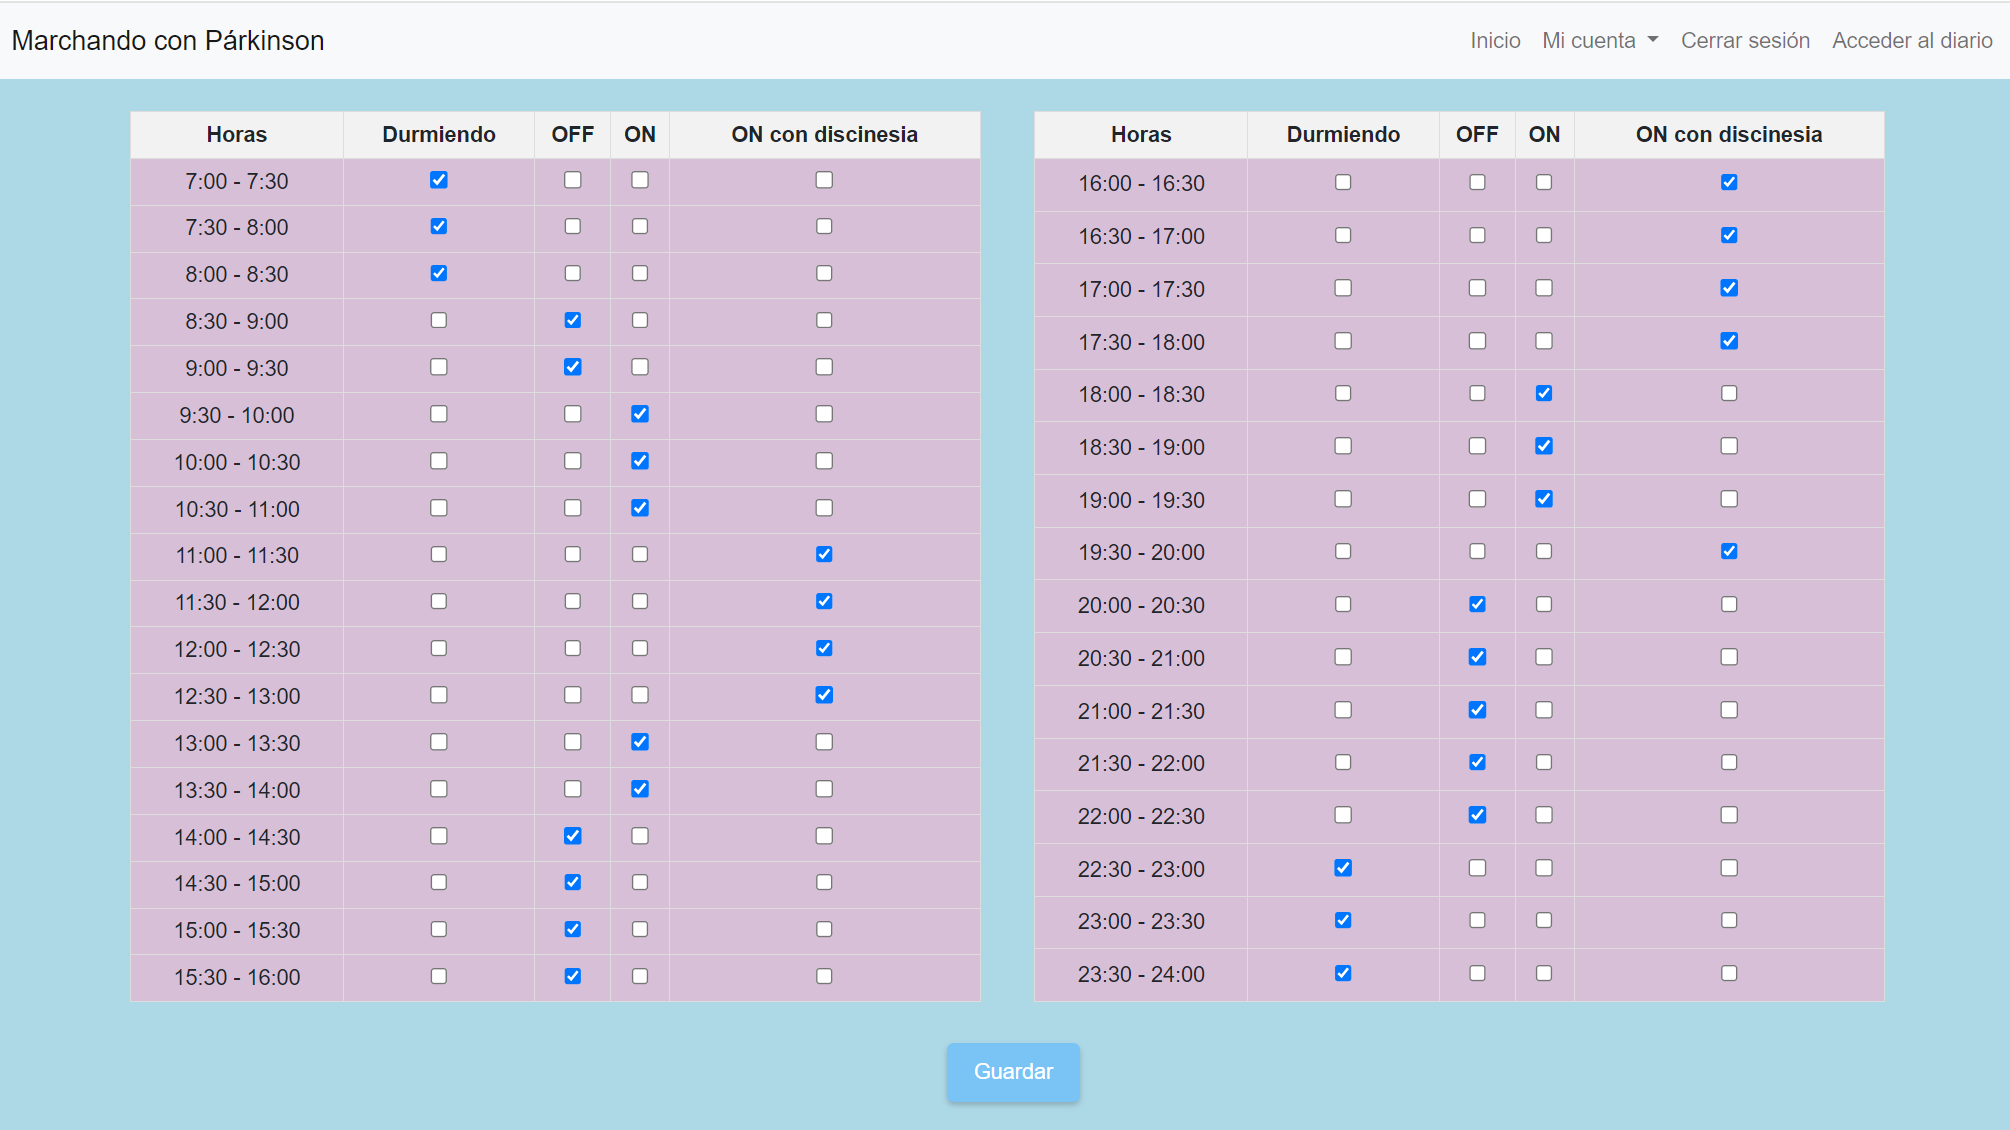
\includegraphics[width=1\textwidth]{img/diariofluc.png}
    \caption{Formulario para rellenar el diario de fluctuaciones (diario de Hauser). Fuente propia.}
    \label{fig:diariofluc}
\end{figure}

\begin{figure}[h]
    \centering
    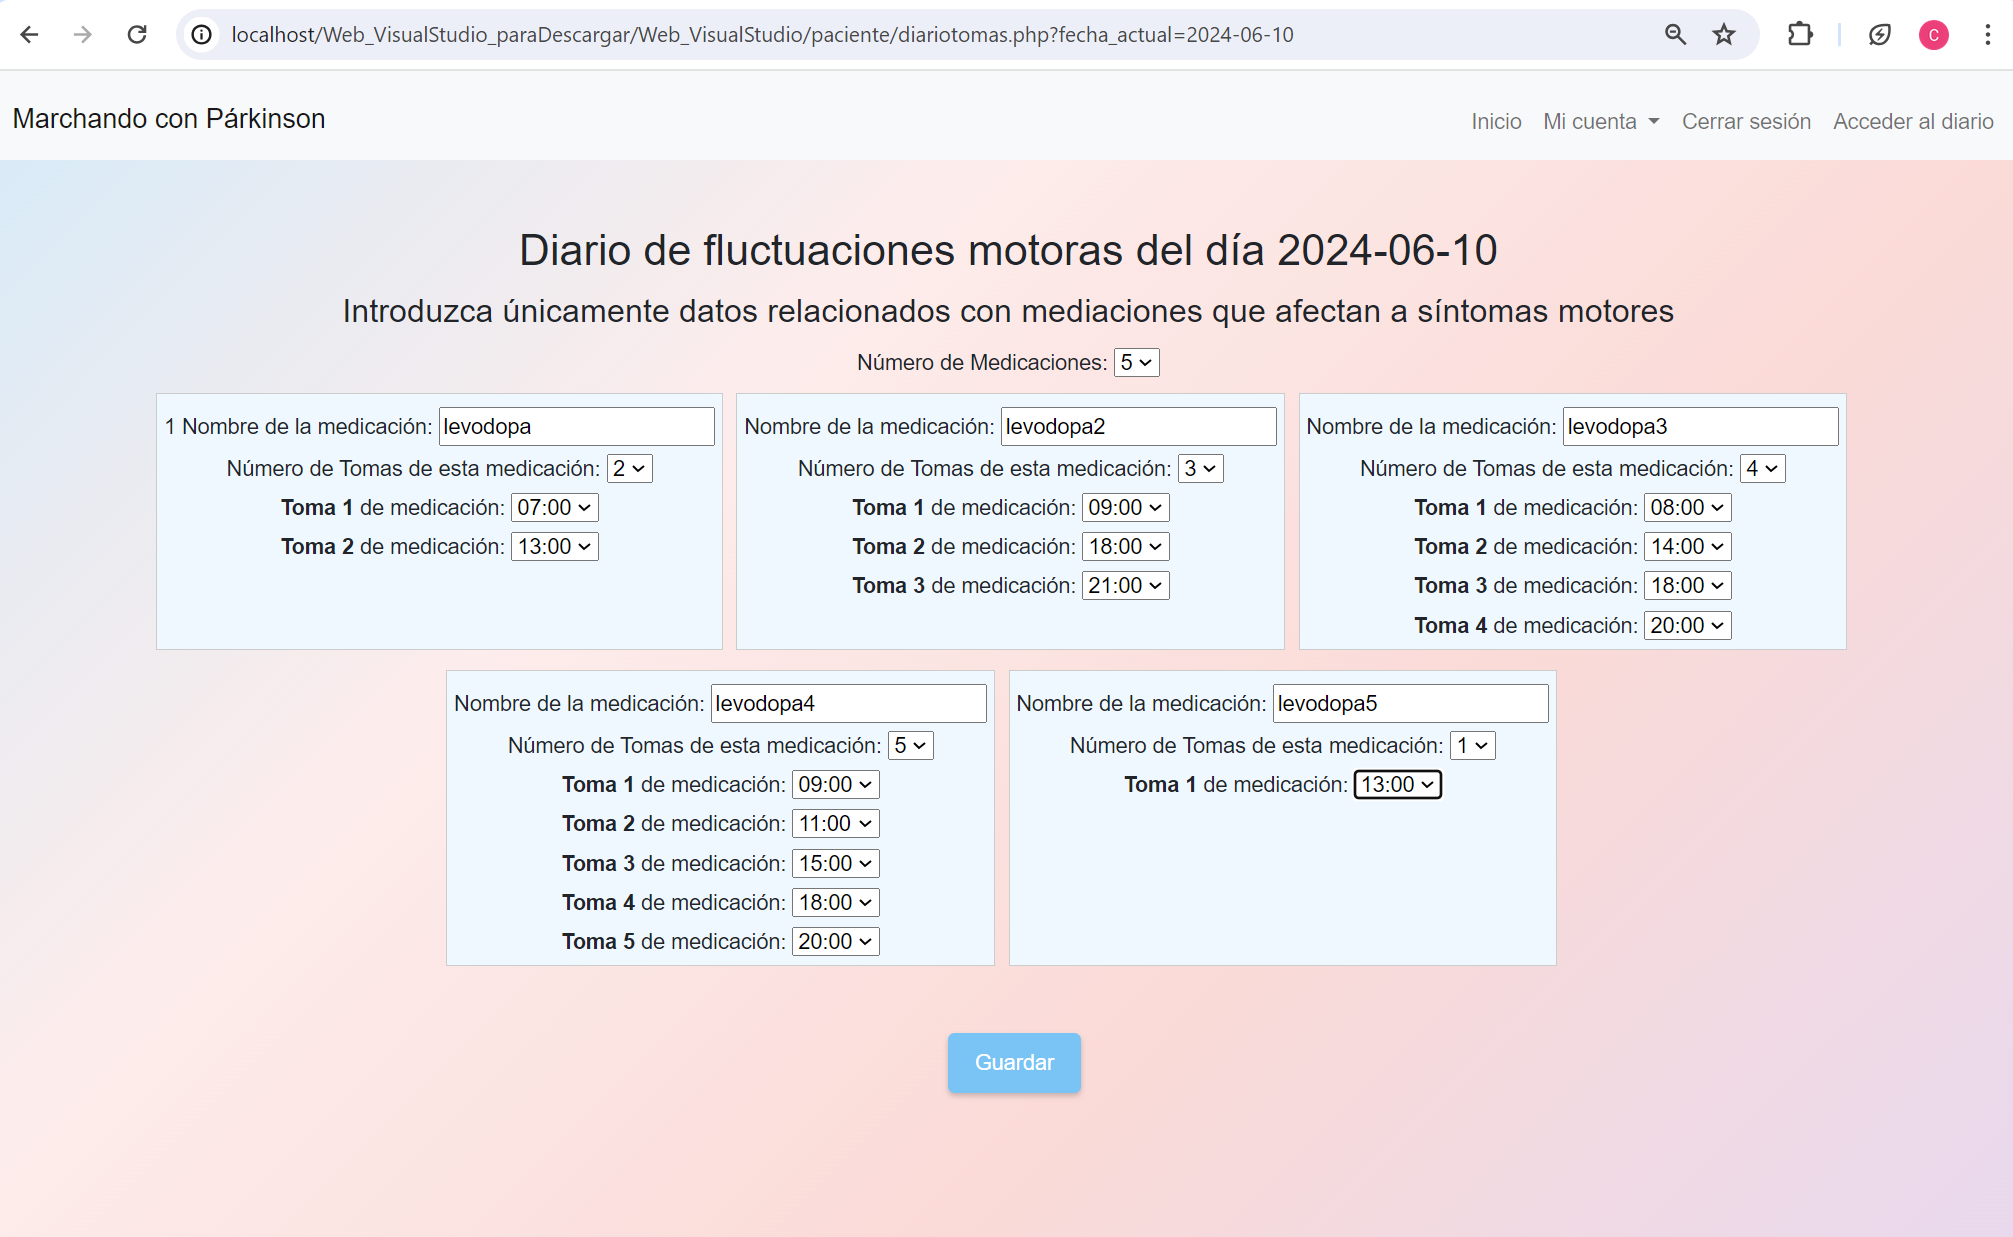
\includegraphics[width=1\textwidth]{img/diariotomas.png}
    \caption{Formulario para rellenar el diario de tomas de medicaciones. Fuente propia.}
    \label{fig:diariotomas}
\end{figure}
Adicionalmente, las funciones del usuario paciente incluyen la visualización de sus gráficas, de forma idéntica a la mostrada para el usuario profesional.
\subsection{Acceso a vídeos de funcionamiento de la aplicación web}
Dentro del repositorio GitHub utilizado, se puede acceder a los vídeos de demostraciones situados dentro de la carpeta 'Vídeos', donde se pueden observar con más detalle el funcionamiento y la demostración de las nuevas funciones de la aplicación.
     
\apendice{Manual del desarrollador/ programador.}

\section{Estructura de directorios}
En el directorio de GitHub \cite{MarcosGordillo2024}, al cual se puede acceder mediante el link \url{https://github.com/cmg1015/TFG_Seguimiento_Parkinson}, se muestran las siguientes carpetas y ficheros:
\begin{itemize}
    \item Carpeta WebVisualStudio: Muestra la carpeta que contiene todos los archivos de código necesarios para el funcionamiento de la aplicación web, incluyendo bibliotecas que se utilizan en dichos códigos. Dentro de la carpeta 'database' se incluye también un documento .sql que contiene la base de datos 'webparkinson', la cual puede importarse utilizando las funciones de phpmyadmin y MySQL disponibles con la aplicación XAMPP. El archivo comprimido WebVisualStudio.rar contiene exactamente los mismos archivos, proporcionando una manera más sencilla de descargar la carpeta.
    \item Carpeta WebVisualStudioCodigo: Contiene tan sólo los archivos de código necesarios para el funcionamiento de la aplicación y el documento .sql con la base de datos 'webparkinson'. El archivo comprimido WebVisualStudioCodigo.zip contiene exactamente los mismos archivos, permitiendo descargarlos de forma más cómoda.
    \item Carpeta Videos: Contiene acceso a los vídeos de pruebas y demostraciones de las nuevas funciones que aporta este proyecto a la solución tecnológica.
    \item Carpeta Arduino: Contiene 2 versiones del script Arduino general (Versión para láser y RTC; Versión guardando la duración de la actividad correctamente y sin utilizar el módulo RTC) y el script de calibración del sensor MPU-6050.
\end{itemize}

A continuación se explicará con más detalle el contenido de la carpeta WebVisualStudioCodigo, profundizando en las funciones de los archivos de código nuevos o modificados y nombrando los archivos conservados desde la versión anterior del proyecto \cite{Martos2024}.
\begin{itemize}
    \item Carpeta 'admin': Esta carpeta contiene los archivos de código .php relacionados con las funciones del usuario de tipo 'administrador'. Estos archivos son:
    \begin{itemize}
        \item 'crearUsuario.php'
        \item 'crearUsuarioHTML.php'
        \item 'eliminarUsuario.php'
        \item 'inicioAdmin.php'
        \item 'listadoPacientes.php'
        \item 'menu.php'
    \end{itemize}
    \item Carpeta 'bluetooth': Esta carpeta contiene los archivos necesarios para la comunicación bluetooth bidireccional entre el dispositivo y la aplicación web y base de datos. Estos archivos son:
    \begin{itemize}
        \item '/bluetooth/ArduinoBridge/bridge.py'
        \item '/bluetooth/ArduinoServer/server.js': Servidor web que utiliza Node.js para gestionar la comunicación y los datos del sistema, programado en JavaScript. Proporciona una serie de endpoints \footnote{Puntos de acceso en una aplicación web que pueden enviar solicitudes para realizar operaciones específicas.}, entre los cuales se modificó el endpoint /guardarActividad para generar datos de fecha y hora de guardado y almacenarlos junto al resto de datos y se creó el endpoint /guardarPersonalización para almacenar datos sobre las pruebas de personalización en la tabla 'actividades' de la base de datos.
    \end{itemize}
    \item Carpeta 'common': Esta carpeta contiene archivos comunes en usuarios de tipo 'profesional' y 'paciente'. Estos archivos son:
    \begin{itemize}
        \item 'actividad.php'
        \item 'actividades.json'
        \item 'actualizarCorreo.php'
        \item 'borrar.py'
        \item 'cambiarContraseña.php'
        \item 'cambiarContraseñaHTML.php'
        \item 'consultaActividades.php'
        \item 'eliminarCuenta.php'
        \item 'estadisticas.py': Este archivo se creó con el objetivo de generar de forma automática gráficas relacionadas con los datos registrados de las actividades.
        \item 'graficas.php': Este archivo se creó para mostrar en la página web la página de acceso a las gráficas. Ejecuta los archivos .py de generación de gráficas y ofrece las opciones de mostrar/esconder cada una de las gráficas.
        \item 'grafdiarios.py': Archivo creado para la generación de una gráfica que muestra los estados de la persona a lo largo de un día (según los datos del diario de fluctuaciones motoras), mostrando también las horas de toma de cada medicación. Esto puede permitir por ejemplo detectar qué medicaciones están teniendo como efecto secundario episodios de discinesia, cuánto tardan en actuar las medicaciones, cuánto dura el efecto...
        \item 'graficasmed.py': Archivo creado para comparar los bloqueos por minuto en actividades realizadas en cada uno de los estados. Este archivo reúne los datos de todas las actividades cuya fecha y hora de realización tenga un estado especificado en el diario de fluctuaciones (es decir, las actividades de los días en que se haya rellenado dicho diario) y hace una comparación entre los bloqueos/minuto totales en actividades realizadas en estado 'on', 'off' y 'on con discinesia'.
        \item 'login.html'
        \item 'login.php'
        \item 'logout.php'
        \item 'pdf.php': Archivo que ejecuta el archivo 'pdf.py' y descarga el pdf generado.
        \item 'pdf.py': Archivo que genera un informe en .pdf con los datos del paciente, estadísticas (medias de los diferentes parámetros) y los datos de las actividades registradas.
        \item 'pdf2.php': Archivo que ejecuta el archivo 'pdf2.py' y descarga el pdf generado.
        \item 'pdf2.py': Archivo que genera un informe en .pdf idéntico al generado por 'pdf.py' incluyendo adicionalmente gráficas.
    \end{itemize}
    \item Carpeta 'database': Contiene el archivo 'webparkinson.sql', que se corresponde con la base de datos utilizado durante el proyecto.
    \item Carpeta 'js'; contiene el archivo 'confirmacion.js'. En este archivo se modificó la función confirmarAccion(accion), añadiendo la acción finalizarPersonalizacion, la cual envía una solicitud al servidor server.js mediante el siguiente link para solicitar el guardado de datos de la prueba de personalización en la tabla 'actividades' de la base de datos:
    
    \url{'http://localhost:3000/guardarPersonalizacion'} 
    \item Carpeta 'paciente': Esta carpeta contiene los archivos relacionados con las funciones del usuario de tipo 'paciente'. Estos archivos son:
    \begin{itemize}
        \item 'diarioestado.php': Formulario creado para permitir rellenar el diario de Hauser o diario de fluctuaciones motoras desde la página web.
        \item 'diarios.php': Archivo creado para dar acceso a los formularios creados por los archivos 'diarioestado.php' y 'diariotomas.php', dando también instrucciones y explicaciones sobre cada uno de ellos y mostrando si han sido ya rellenados o no.
        \item 'diariotomas.php': Formulario creado para permitir rellenar el diario de tomas de medicaciones desde la página web.
        \item 'inicioPaciente.php'
        \item 'menu.php'
        \item 'procesardiario.php': Archivo creado para procesar las respuestas del formulario 'diarioestados.php', almacenándolas en la base de datos.
        \item 'procesardiario2.php': Archivo creado para procesar las respuestas del formulario 'diariotomas.php', almacenándolas en la base de datos.
    \end{itemize}
    \item Carpeta 'profesional': Esta carpeta contiene archivos relacionados con las funciones del usuario de tipo 'profesional'. Estos archivos osn:
    \begin{itemize}
        \item 'asignarPaciente.php'
        \item 'infoPaciente.php'
        \item 'inicioProfesional.php'
        \item 'menu.php'
        \item 'mostrarPacientes.php'
        \item 'nuevoPaciente.php'
        \item 'nuevoPacienteHTML.php'
        \item 'pautas.php': Este archivo se creó para mostrar un formulario, similar al mostrado en /paciente/diariotomas.php, para asignar una pauta de medicación a un paciente en concreto del cual se especifica el número de identificación.
        \item 'personalizarbloqueo.php' Este archivo se creó para permitir la realización de pruebas de personalización del tiempo a partir del cual se detecta un congelamiento de la marcha. A partir de los datos recogidos relativos a los segundos que tarda de media el paciente en dar un paso se calcula el número de segundos óptimo, el cual se pasa como comando al servidor web server.js en el link \url{'http://localhost:3000/datos'}. Esto permitirá el envío de dichos comandos al script arduino, que adaptará el tiempo de detección de congelamiento de la marcha acorde a ellos.
        \item 'procesarpautas.php'; Archivo creado para procesar las respuestas al formulario 'pautas.php' y almacenarlas en la base de datos.
        \item 'quitarPaciente.php'
    \end{itemize}
\end{itemize}

\section{Pruebas del sistema}
La validación de la interfaz por parte de potenciales usuarios se detalla en el anexo G, mediante la realización de una encuesta. Por otro lado, la validación del funcionamiento del sistema puede comprender varios puntos:
\begin{itemize}
    \item Comprobación de la correcta conexión del dispositivo bluetooth y comunicación bidireccional de comandos: Tras conectar el dispositivo mediante bluetooth y ajustar el puerto COM tal y como se describe en la figura \ref{fig:bridgepy}; es necesario comprobar que se está llevando a cabo una correcta comunicación con el dispositivo Arduino. En caso de éxito, al ejecutar el archivo 'bridge.py' tras haber ejecutado el servidor web con el comando node server.js (tal y como se explica en el anexo B), deberíamos observar en la terminal de Visual Studio algo similar a lo mostrado en la figura \ref{fig:bridgeejecutando}.
    \item Comprobación del correcto funcionamiento de las distintas funciones de la aplicación web: Esto puede realizarse mediante comprobaciones con datos ficticios, tal y como se muestra en los Vídeos de demostraciones del repositorio GitHub \cite{MarcosGordillo2024}.
\end{itemize}

\section{Instrucciones para la modificación o mejora del proyecto.}
Con el objetivo de proseguir con la mejora del proyecto, pueden tenerse en cuenta las guías generales sugeridas en el apartado 'Líneas futuras' de la memoria del proyecto. En este apartado se presentan algunas sugerencias más técnicas:
\begin{itemize}
    \item Automatizar los procesos que deben llevarse a cabo para asegurar la conexión del dispositivo con la aplicación de forma manual en Visual Studio: La ejecución del archivo 'bridge.py' o el arranque del servidor web server.js podrían realizarse de forma automática al iniciar una actividad que requiera la conexión del dispositivo, dejando como único paso manual la conexión del dispositivo al ordenador.
    \item Ajustar el frontend de la página web para hacerlo responsivo: Ajustar los estilos de la aplicación web de modo que al acceder desde diferentes tamaños de pantalla se muestre el contenido de forma adecuada. Actualmente tan sólo algunos estilos funcionan de manera responsiva, haciendo que el acceso a la web desde dispositivos de tamaños diferentes o simplemente con la pantalla minimizada resulte complicado. Esto puede realizarse por ejemplo ajustando los estilos CSS expresados en pixels a porcentajes de la pantalla o adaptando el diseño de la web a las dimensiones de la pantalla en que se muestra.
    \item Añadir una tarjeta SD al dispositivo, permitiendo almacenar los datos de actividades durante un periodo de tiempo y posteriormente cargarlos en la base de datos, pudiendo visualizar y analizar dichos datos.
    \item Añadir sensores MPU-6050, ya sea utilizando un duplicado del sensor en la ubicación actual, aportando una mayor precisión y un indicador fiable de cuándo es necesario calibrarlos u añadiendo sensores en otras ubicaciones, como dentro del cinturón o en el tobillo derecho.
\end{itemize}

\apendice{Descripción de adquisición y tratamiento de datos}
En este apéndice se describe la naturaleza, almacenamiento y utilidad de los datos recogidos por la solución tecnológica propuesta. Se detalla la composición de la base de datos utilizada y la utilidad clínica de los datos almacenados.

\section{Descripción formal de los datos}
Esta solución tecnológica procesa mayoritariamente 2 tipos de datos: datos sobre parámetros de la marcha del paciente, obtenidos a partir de las funciones de acelerómetro y giroscopio sensor MPU-6050 incluido en el dispositivo hardware y datos sobre la toma de medicaciones y el estado o fluctuaciones motoras del paciente, registrados en los diarios que el paciente puede completar en la aplicación web.

Durante el desarrollo del dispositivo no se han utilizado datos reales de pacientes, por lo cual no ha sido necesario rellenar documentos del comité ético, consentimientos o crear políticas de privacidad de los datos.

Los datos obtenidos por el dispositivo y almacenados desde la aplicación web han sido almacenados en la base de datos 'webparkinson', cuya estructura se detalla a continuación.
\subsection{Base de datos 'webparkinson'}
La base de datos 'webparkinson' está compuesta por 8 tablas. 4 de estas tablas, las correspondientes con el almacenamiento de actividades, datos de pacientes, datos de usuarios y relaciones profesional/paciente fueron creadas y explicadas en el TFG \cite{Martos2024}. El propósito de las 4 tablas restantes es explicado a continuación:
\begin{itemize}
    \item La tabla 'pautas' almacena los datos sobre la pauta de medicación asignada a un paciente que el profesional introduce desde la aplicación web. Estos datos servirán posteriormente para que dicho paciente los tenga como respuesta predeterminada al rellenar el diario de toma de medicaciones, agilizando por tanto el proceso. 

    Esta tabla está compuesta por 9 columnas:
    \begin{enumerate}
        \item La primera columna representa el id de la tabla, es decir, un número asignado de forma automática que representa el número de la fila insertada en la tabla. Es único y por tanto se utiliza como clave primaria de la tabla. Es de tipo int (número entero)
        \item La columna 'paciente' sirve para guardar el número de identificación del paciente del cual se están guardando registros.
        \item La columna 'nummed' representa el número de la medicación que representa cada fila. Una pauta de medicaciones puede incluir entre 1 y 5 medicaciones diferentes, las cuales se almacenan como filas separadas. La columna 'nummed' nos permite rellenar de forma predeterminada o no mostrar los diferentes campos del fomulario en el diario de medicaciones del paciente teniendo en cuenta el número de medicaciones introducidas en la pauta. 
        \item La columna 'medicacion' almacena el nombre de cada medicación. Se trata de una columna de tipo 'text'.
        \item Las columnas hora 1, hora 2, hora 3, hora 4 y hora 5 almacenarán un valor de tipo 'date' en caso de que la medicación correspondiente tenga dicha hora de toma (por ejemplo si la medicación tiene 3 horas de toma hora 1 hora 2 y hora 3 tendran valores tipo 'date'), mientras que el resto de columnas permanecerán vacías.
    \end{enumerate}
    \item La tabla 'personalizacion' almacena los datos de las actividades realizadas durante pruebas de personalización. Tiene la misma estructura que la tabla 'actividades':
    \begin{enumerate}
        \item La primera columna es la clave primaria de la tabla y representa el id de la tabla: un número que se incrementa de forma automática con la adición de una nueva fila en la tabla.
        \item El id del paciente almacena el número de identificación del paciente que está realizando la actividad
        \item El número de bloqueos totales durante la actividad, se almacena en un dato de tipo 'int.'
        \item La velocidad media durante la actividad, se almacena en un dato de tipo 'decimal (10,2)'.
        \item El número de pasos realizados durante la actividad se almacena en un dato de tipo 'int'.
        \item La duración total de la actividad en minutos se almacena en un dato de tipo 'float'.
    \end{enumerate}
    \item La tabla 'diario' almacena los datos registrados en el diario de fluctuaciones motoras, en el que se guardan para una fecha determinada el estadod el paciente (on, off, on con disicnesia o durmiendo) para intervalor horarios de media hora entre las 7:00 y las 00:00. En esta tabla cada intervalo horario se almacena como una fila distinta. La estructura de la tabla es:
    \begin{enumerate}
        \item Número de identificación de la tabla: número incrementado de forma automática con la adición de una nueva fila en la tabla que funciona como clave primaria. Es un dato de tipo 'int'.
        \item Fecha: fecha en la cual se registra el diario. Es un dato de tipo 'date'.
        \item Hora: Hora de inicio del intervalo horario registrado. Es un dato de tipo 'time'.
        \item Durmiendo: Dato de tipo 'int' que será igual a 1 en caso de que durmiendo sea el estado seleccionado para la franja horaria o 0 en caso contrario.
        \item Off status: Dato de tipo 'int' que será igual a 1 en caso de que 'off' sea el estado seleccionado para la franja horaria o 0 en caso contrario.
        \item On status: Dato de tipo 'int' que será igual a 1 en caso de que 'on' sea el estado seleccionado para la franja horaria o 0 en caso contrario.
        \item Ondis status: Dato de tipo 'int' que será igual a 1 en caso de que 'on con discinesia' sea el estado seleccionado para la franja horaria o 0 en caso contrario.
    \end{enumerate}
    \item La tabla 'diario2' almacena los datos registrados en el diario de tomas de medicación, en el que se guardan para cada fecha las diferentes medicaciones tomadas (1 a 5) y las diferentes tomas (1 a 5) para cada una de las medicaciones. Cada medicación diferente supondrá una nueva fila en la tabla.
    \begin{enumerate}
        \item Número de identificación de la tabla: número incrementado de forma automática con la adición de una nueva fila en la tabla que funciona como clave primaria. Es un dato de tipo 'int'.
        \item Fecha: fecha en la cual se registra el diario. Es un dato de tipo 'date'.
        \item Medicación: nombre de la medicación de la cual se registra(n) toma(s)
        \item Hora 1, hora 2, hora 3, hora 4 y hora 5: Horas de tomas de la medicación. En caso de que la medicación requiera menos de 5 tomas el resto de tomas quedarán sin registrar (con valor null o 00:00:00)
    \end{enumerate}
\end{itemize}
\section{Descripción clínica de los datos.}
El registro de parámetros de la marcha mediante el acelerómetro y giroscopio del sensor MPU-6050, tal y como se desarrolló en los trabajos \cite{Martos2024} \cite{Gonzalez2023}, proporciona valiosa información acerca de la evolución de los síntomas motores de la marcha en pacientes con párkinson. La visualización de estos datos mediante gráficas permite al profesional una herramienta adicional para la monitorización de dichos síntomas.

Por otro lado, el registro de un diario de Hauser \cite{hauser2000home} o diario de fluctuaciones; aporta información subjetiva del paciente acerca de su estado\footnote{Estado ON: Las medicaciones están haciendo efecto y el paciente presenta movimientos más ágiles. Estado ON con discinesia: Adicionalmente el paciente presenta episodios de movimientos involuntarios. Estado OFF: Las medicaciones no están haciendo efecto, el paciente presenta sintomatología motora agravada.} y los síntomas motores que presenta en cada momento del día. Esto resulta una forma efectiva del seguimiento del efecto de medicaciones que ha sido ampliamente utilizada tanto en ensayos clínicos como en consultas de pacientes para evaluar el efecto de una nueva medicación a lo largo de un intervalo de tiempo. Combinar estos datos con las horas de toma de las medicaciones por parte del paciente y los datos registrados en las actividades realizadas permite al profesional evaluar qué medicaciones provocan efectos de discinesia en el paciente, la duración del efecto de estas medicaciones...

En definitiva, garantizar una monitorización exhaustiva de los síntomas motores en pacientes con Párkinson facilita las decisiones del profesional sanitario a la hora de adaptar la pauta de medicaciones a la progresión de la enfermedad y las circunstancias del paciente

\apendice{Manual de especificación de diseño}

\section{Diseño arquitectónico}
\subsection{Colocación de los elementos hardware}
La figura \ref{fig:esquemahardware} es un esquema de los componentes hardware y su colocación propuesta en el prototipo, dentro de una riñonera en la cual se sitúan los componentes en 2 capas y una tobillera. Las conexiones entre distintos componentes hardware se representan de forma simplificada mediante flechas moradas. 

Las plataformas sin etiquetar sobre las que están conectados los pulsadores ON/OFF y el sensor MPU-6050 representan dos mitadas de una miniboard (miniplaca de pruebas), la cual se utiliza para conectar estos componentes de forma reversible, permitiendo la corrección de errores o el rediseño del circuito.
\begin{figure}[h]
    \centering
    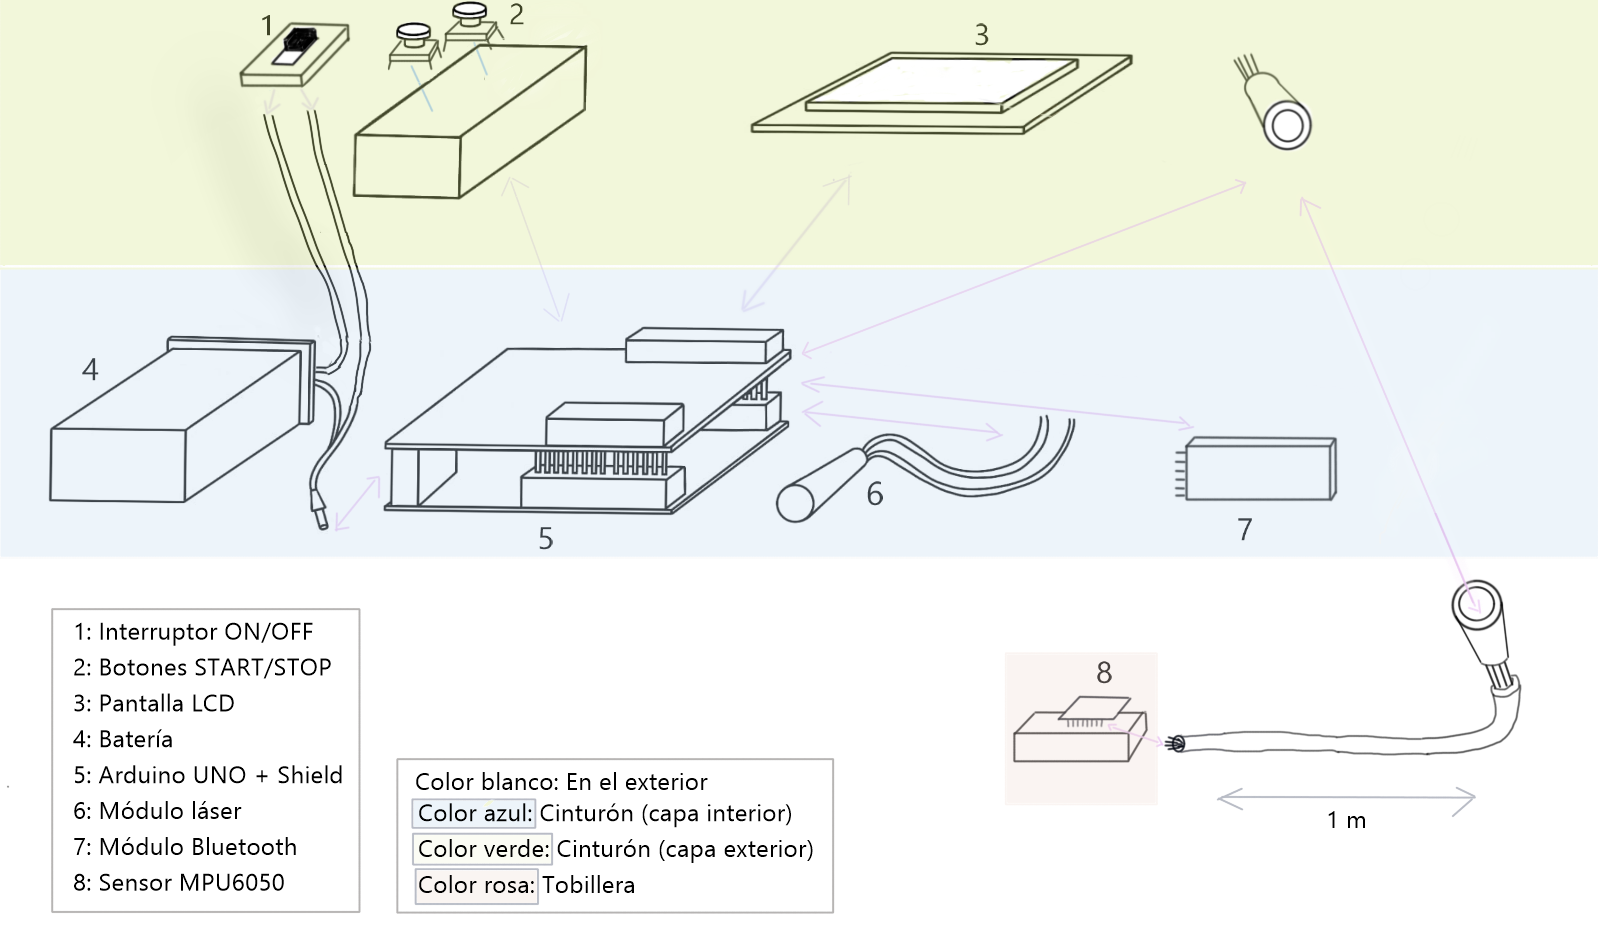
\includegraphics[width=1\textwidth]{img/esquemahardware.png}
    \caption{Esquema del diseño del hardware. Fuente propia}
    \label{fig:esquemahardware}
\end{figure}
\subsection{Conexiones de elementos hardware}
El esquema \ref{fig:circuito} refleja las conexiones requeridas en el circuito que une la placa Arduino UNO con los diferentes módulos y componentes hardware. Es importante recalcar que varios pines de la placa son la fuente de múltiples conexiones, por lo cual se utilizó un Arduino Proto Shield conectado a la placa con el objetivo de aumentar los puntos de conexión a dichos pines mediante soldaduras.
\begin{sidewaysfigure}[h]
    \centering
    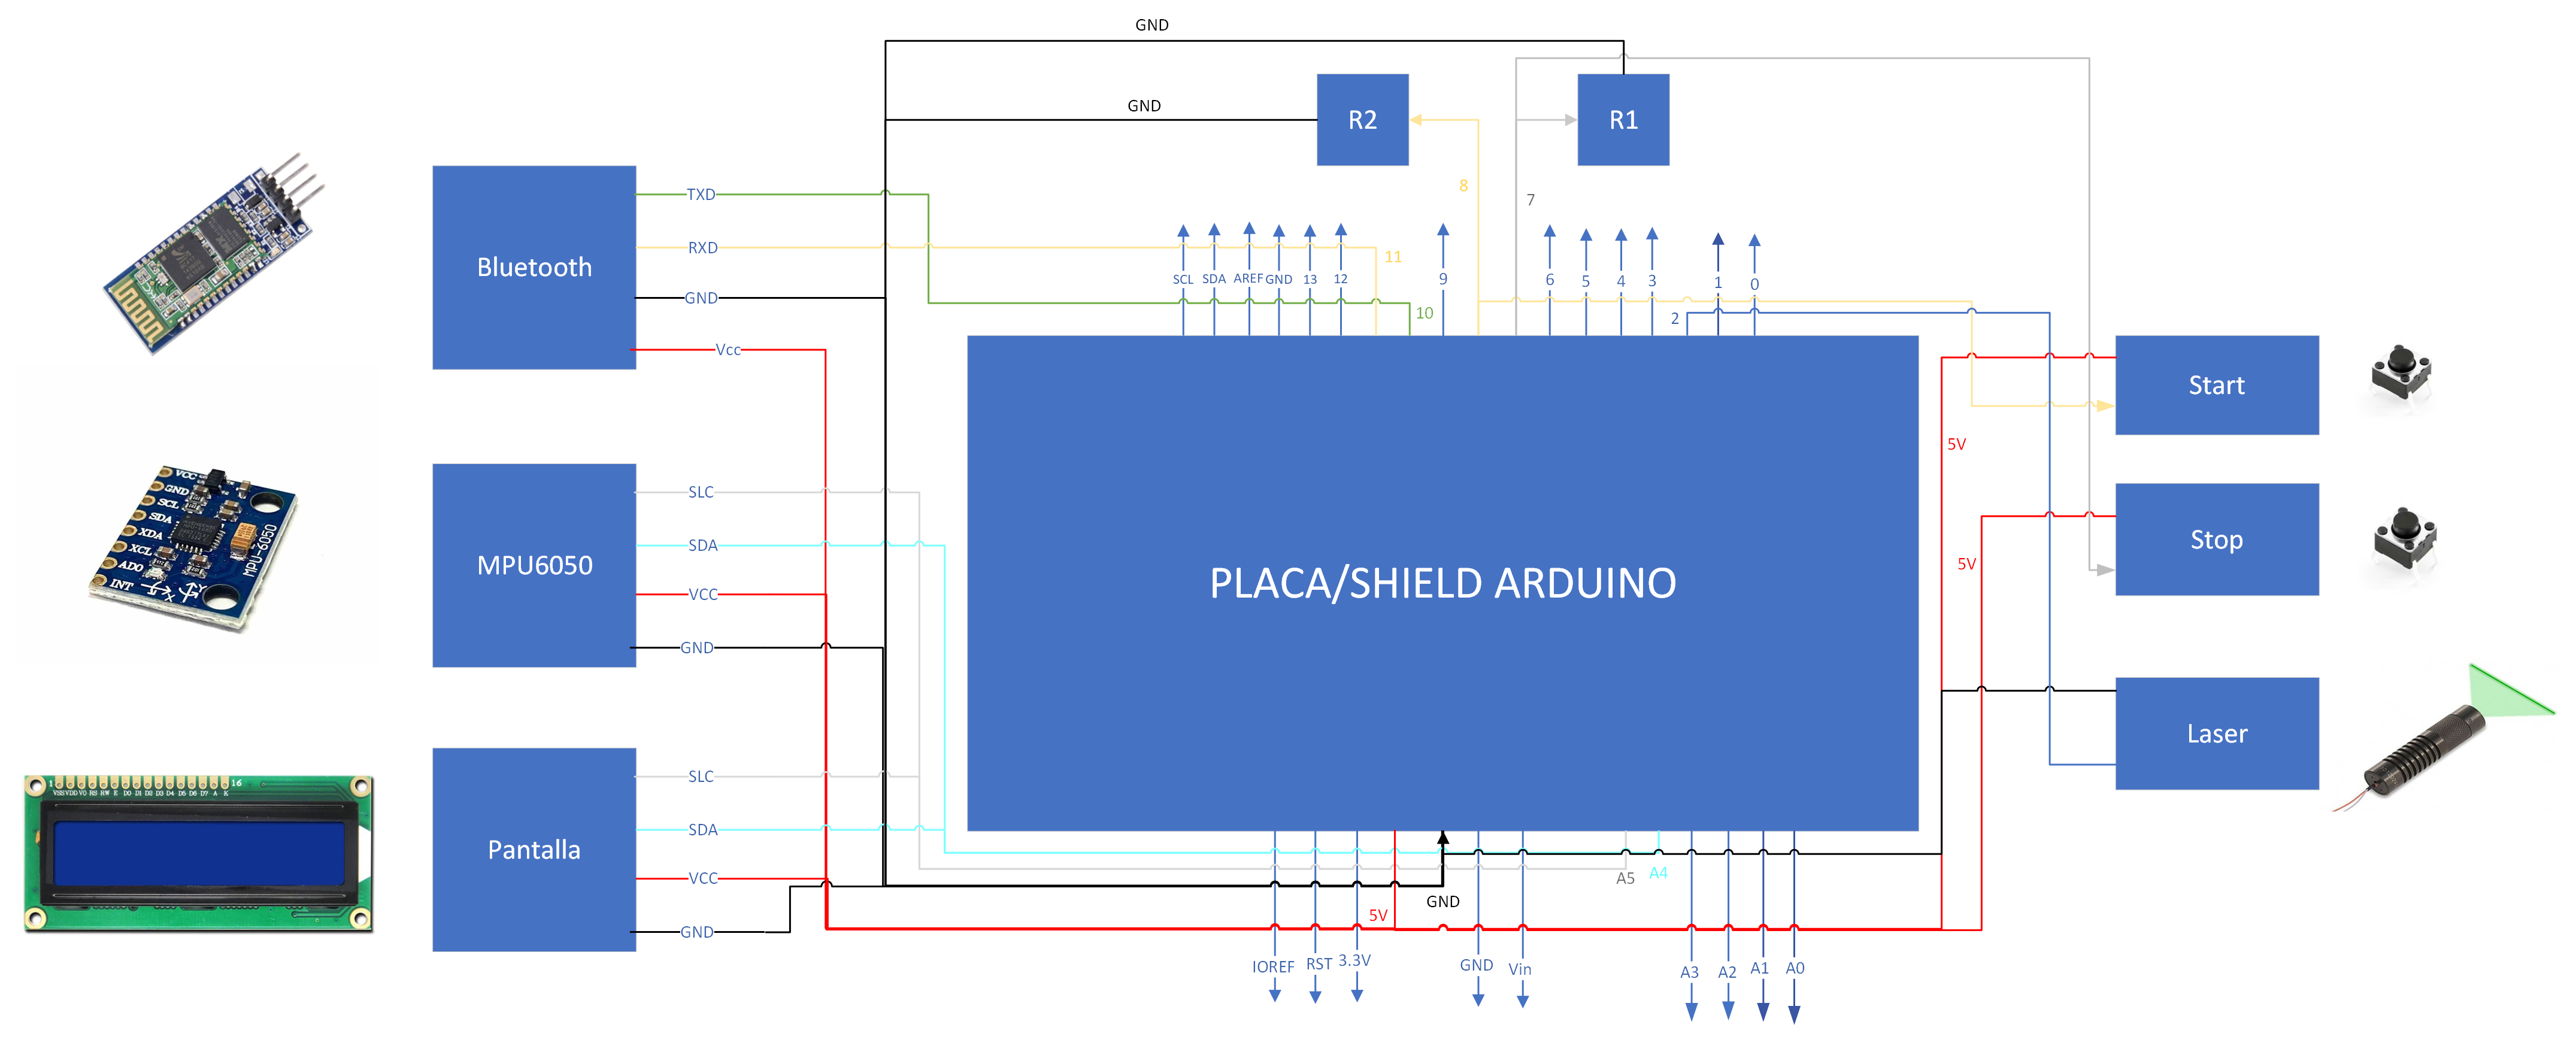
\includegraphics[width=1\textwidth]{img/circuito.png}
    \caption{Esquema de las conexiones de elementos hardware a la placa Arduino UNO. Fuente propia}
    \label{fig:circuito}
\end{sidewaysfigure}

Las conexiones más complicadas son detalladas en las figuras \ref{fig:conexionmpu} (conexión del sensor MPU-6050) \ref{fig:conexionpantalla} (conexión de la pantalla LCD) \ref{fig:conexionpulsadores} (conexión de los pulsadores ON/OFF). Es importante tener en cuenta que estas imágenes son tan sólo una simplificación de las conexiones, ya que tanto los cables como las resistencias que parten de la placa Arduino están soldados en realidad al Proto Shield de Arduino. Adicionalmente, la conexión entre la placa y el sensor MPU-6050 se realiza mediante un cable multihilo, conectado en un extremo a 4 cables provenientes de la placa mediante un conector y en el otro extremo a la mitad de la miniplaca de pruebas donde se conecta el sensor.
\begin{figure}[h]
    \centering
    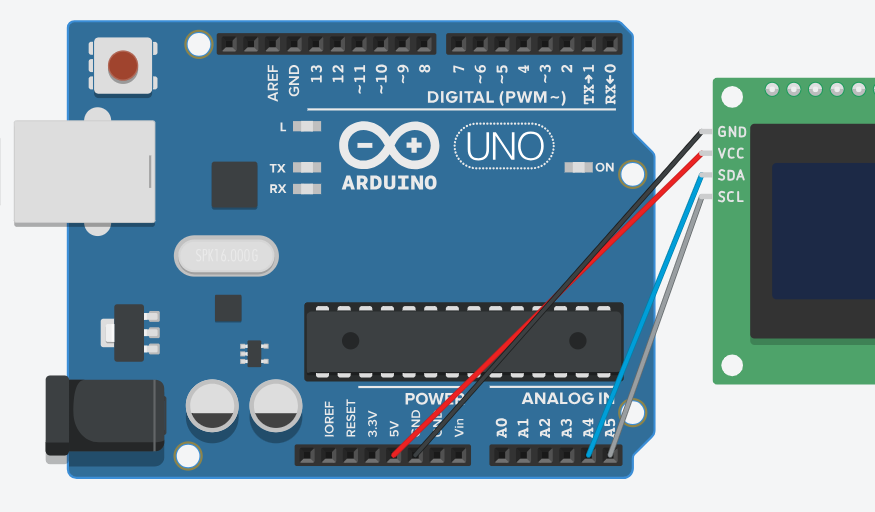
\includegraphics[width=1\textwidth]{img/conexionpantalla.png}
    \caption{Esquema de las conexiones entre la pantalla LCD la placa Arduino UNO mediante el protocolo I2C. Fuente propia}
    \label{fig:conexionpantalla}
\end{figure}
\begin{figure}[h]
    \centering
    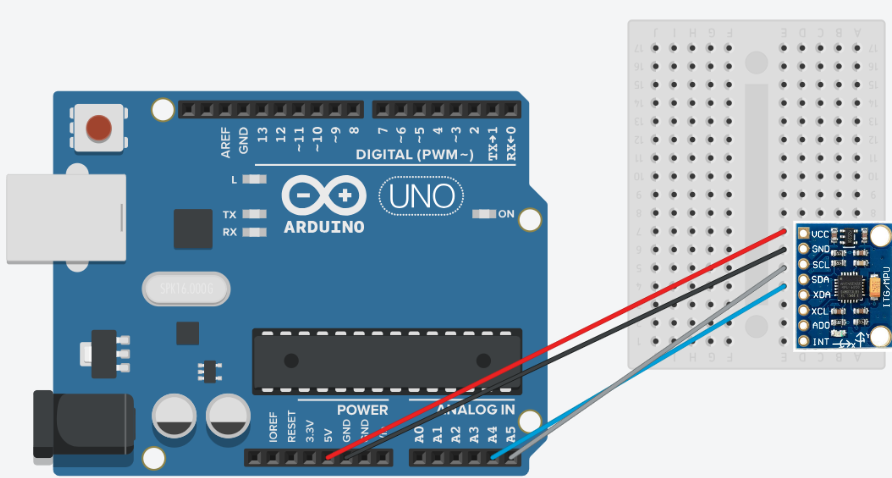
\includegraphics[width=1\textwidth]{img/Conexionmpu.png}
    \caption{Esquema de las conexiones entre el sensor MPU-6050 y la placa Arduino UNO. Fuente propia}
    \label{fig:conexionmpu}
\end{figure}
\begin{figure}[h]
    \centering
    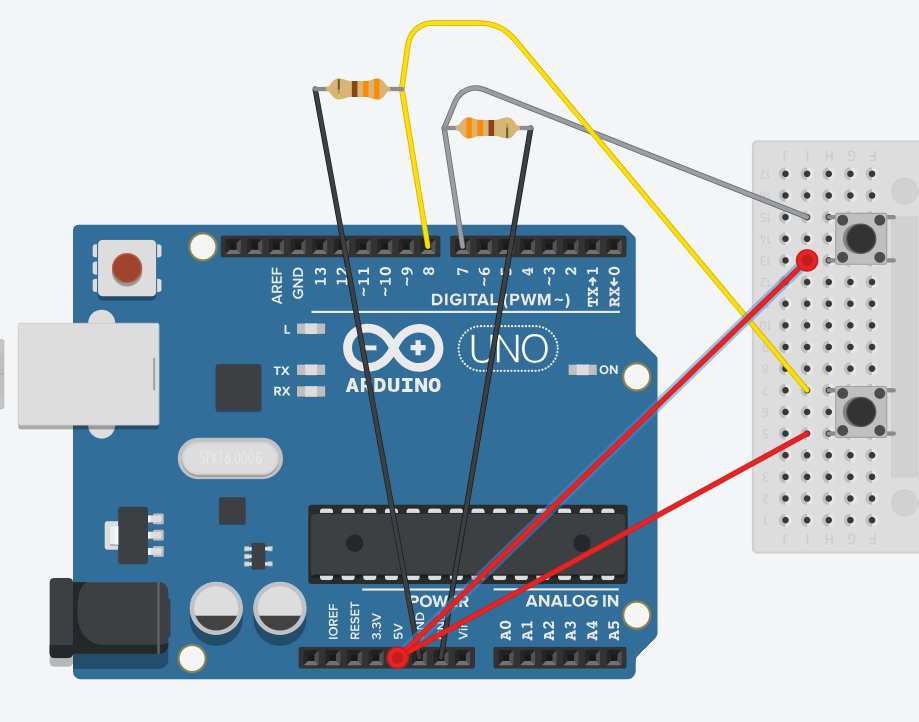
\includegraphics[width=1\textwidth]{img/conexionpulsadores.png}
    \caption{Esquema de las conexiones de los pulsadores ON/OFF a la placa Arduino UNO. Fuente propia}
    \label{fig:conexionpulsadores}
\end{figure}
\subsection{Diagrama de despliegue}
El diagrama de despliegue mostrado en la figura \ref{fig:diagramadespliegue} muestra la estructura y conexiones de los elementos hardware y software que forman el prototipo presentado. Los usuarios acceden mediante su navegador web a la aplicación web, desde la cual hacen uso de diferentes funciones, algunas de las cuales implican el almacenamiento de datos en las tablas de la base de datos 'webparkinson'. Por otro lado, el dispositivo hardware se comunica con el servidor web de la aplicación para enviar datos recogidos por el sensor en tiemo real, recibiendo también información de dicho servidor como comandos.
\begin{figure}[h]
    \centering
    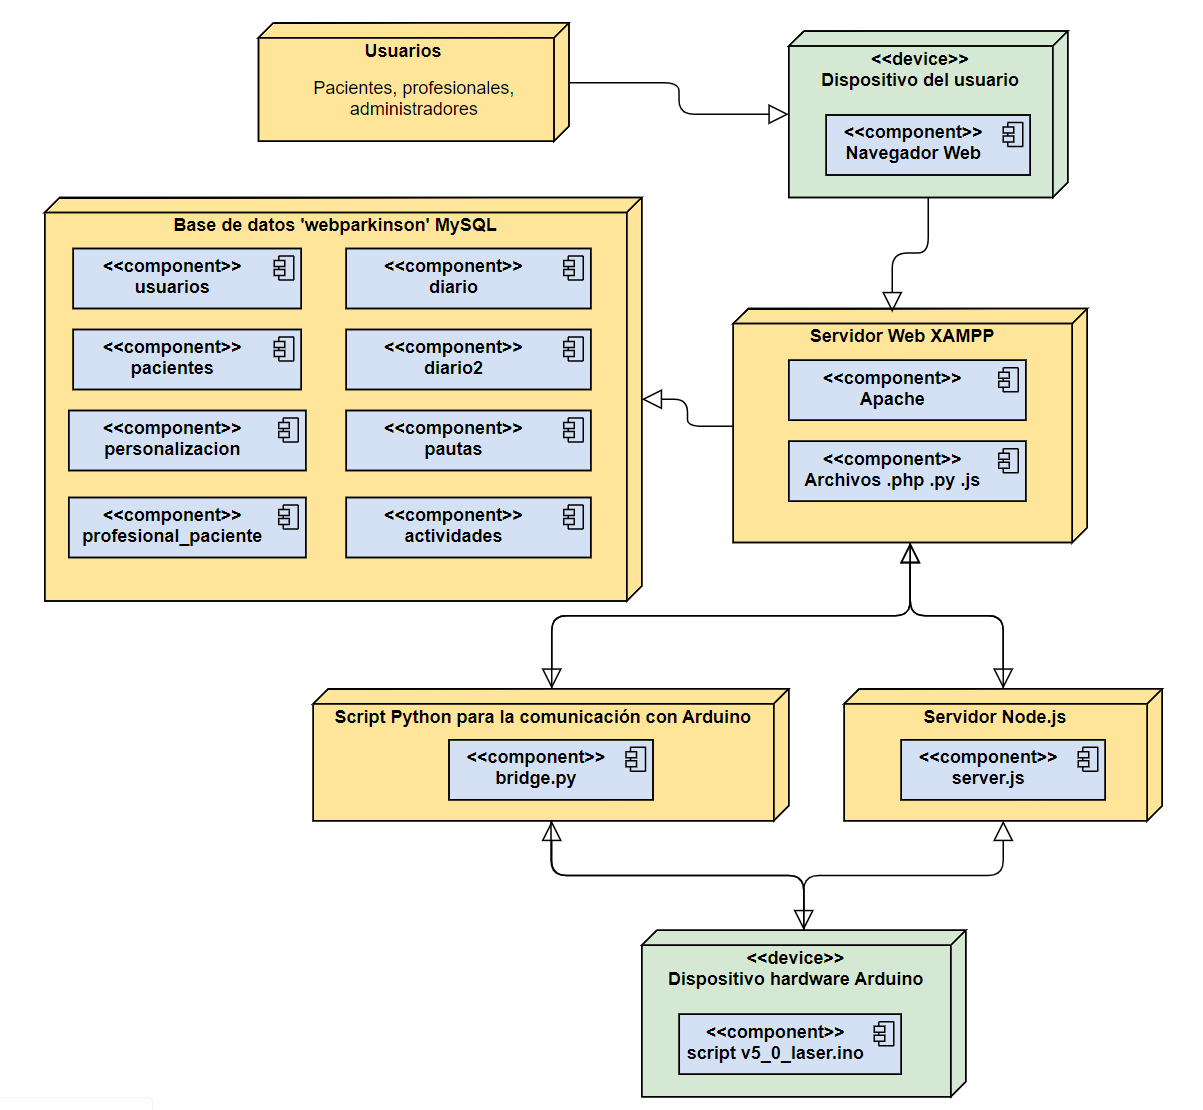
\includegraphics[width=1\textwidth]{img/diagramadespliegue.png}
    \caption{Diagrama de despliegue del sistema. Fuente propia}
    \label{fig:diagramadespliegue}
\end{figure}



\apendice{Especificación de Requisitos}
Un caso de uso puede definirse como una 'secuencia de acciones realizadas por el sistema, que producen un resultado observable y valioso para un usuario en particular'\cite{Cillero2024}. Los diagramas de casos de uso mostrados a continuación ilustran estas acciones del sistema relacionadas con los 3 tipos de usuario contemplados en la presente solución tecnológica: Paciente (persona con Enfermedad de Párkinson), profesional (profesional sanitario) y administrador.
\section{Diagramas de casos de uso}
Con el objetivo de mostrar las mejoras en la aplicación web que se han realizado durante este proyecto y dar también un contexto general del funcionamiento total de la aplicación, se muestran una serie de diagramas de casos de uso.

Las mejoras realizadas en la aplicación web afectan únicamente a los usuarios de tipo 'paciente' y 'profesional'. Debido a ello se muestra en la figura \ref{fig:Casosdeuso} un diagrama de casos de uso relacionado con estos dos tipos de usuarios.
\begin{figure}[h]
    \centering
    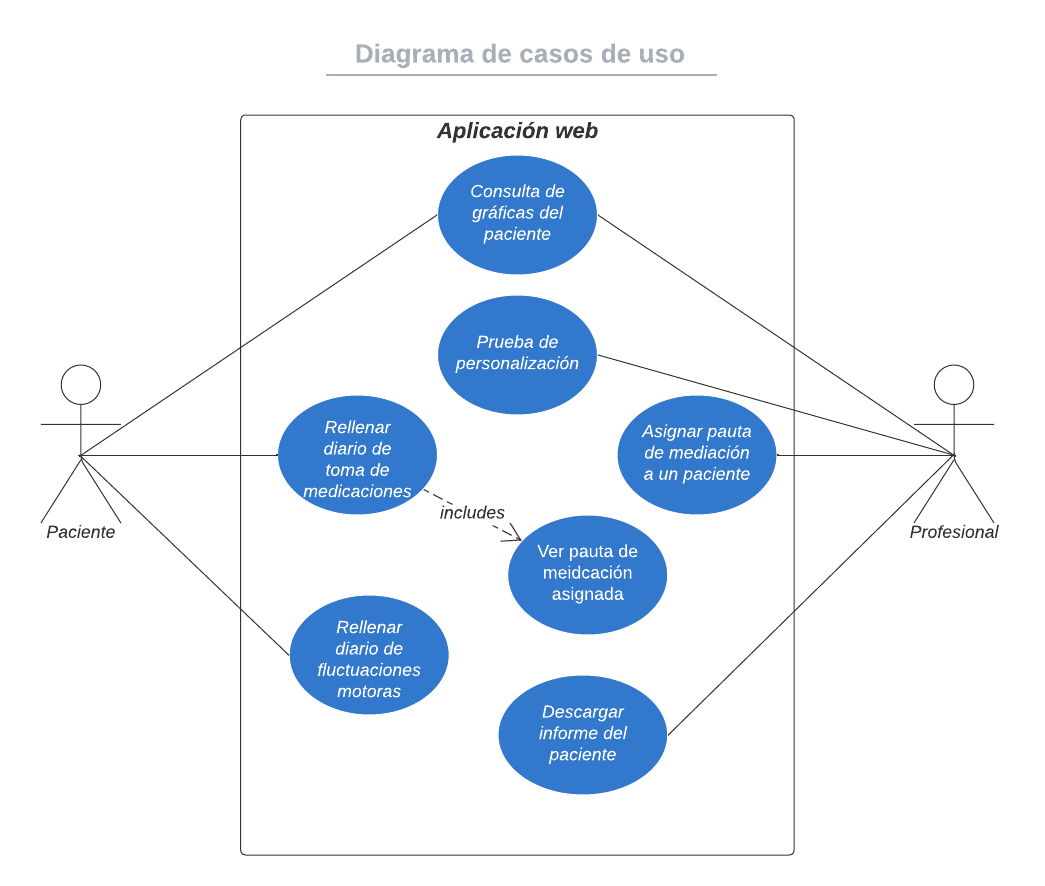
\includegraphics[width=1\textwidth]{img/Casosdeuso.png}
    \caption{Casos de uso de las nuevas funciones de la app}
    \label{fig:Casosdeuso}
\end{figure}

Los casos de uso con las funciones totales comunes para todos los usuarios se  mantienen respecto al TFG \cite{Martos2024}, y se muestran en la figura \ref{fig:Casosusotodos}. Los casos de uso incluyendo las funciones exclusivas para el usuario administrador también permanecen intactas desde el proyecto \cite{Martos2024}, y se muestran en la figura \ref{fig:Casosusoadmin}.

Los casos de uso relativos a las funciones de usuarios de tipo profesional y paciente han sido ampliad0s a partir de los descritas el proyecto \cite{Martos2024}, resultando en el diagrama mostrado en la figura \ref{fig:Casospacienteprof}
\begin{figure}[h]
    \centering
    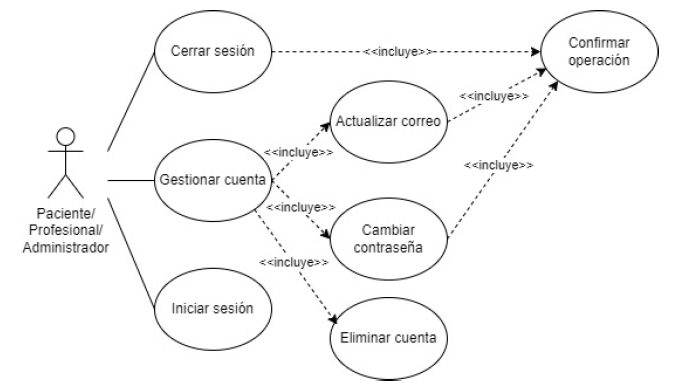
\includegraphics[width=1\textwidth]{img/casosinestodos.png}
    \caption{Casos de uso para todos los usuarios \cite{Martos2024}}
    \label{fig:Casosusotodos}
\end{figure}

\begin{figure}[h]
    \centering
    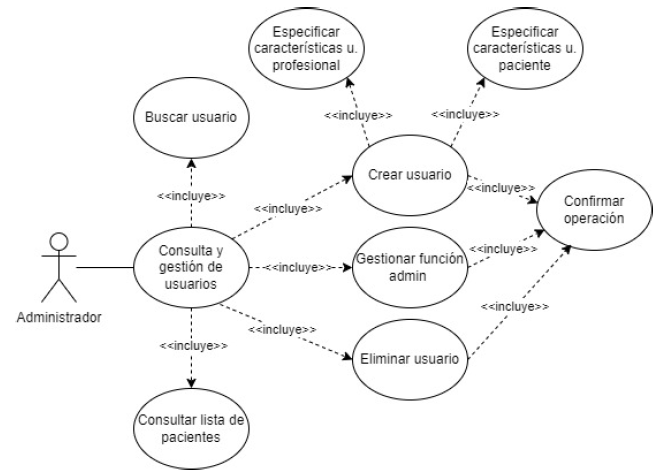
\includegraphics[width=1\textwidth]{img/casosinesadmin.png}
    \caption{Casos de uso para el usuario de tipo 'Administrador' \cite{Martos2024}}
    \label{fig:Casosusoadmin}
\end{figure}

\begin{figure}[h]
    \centering
    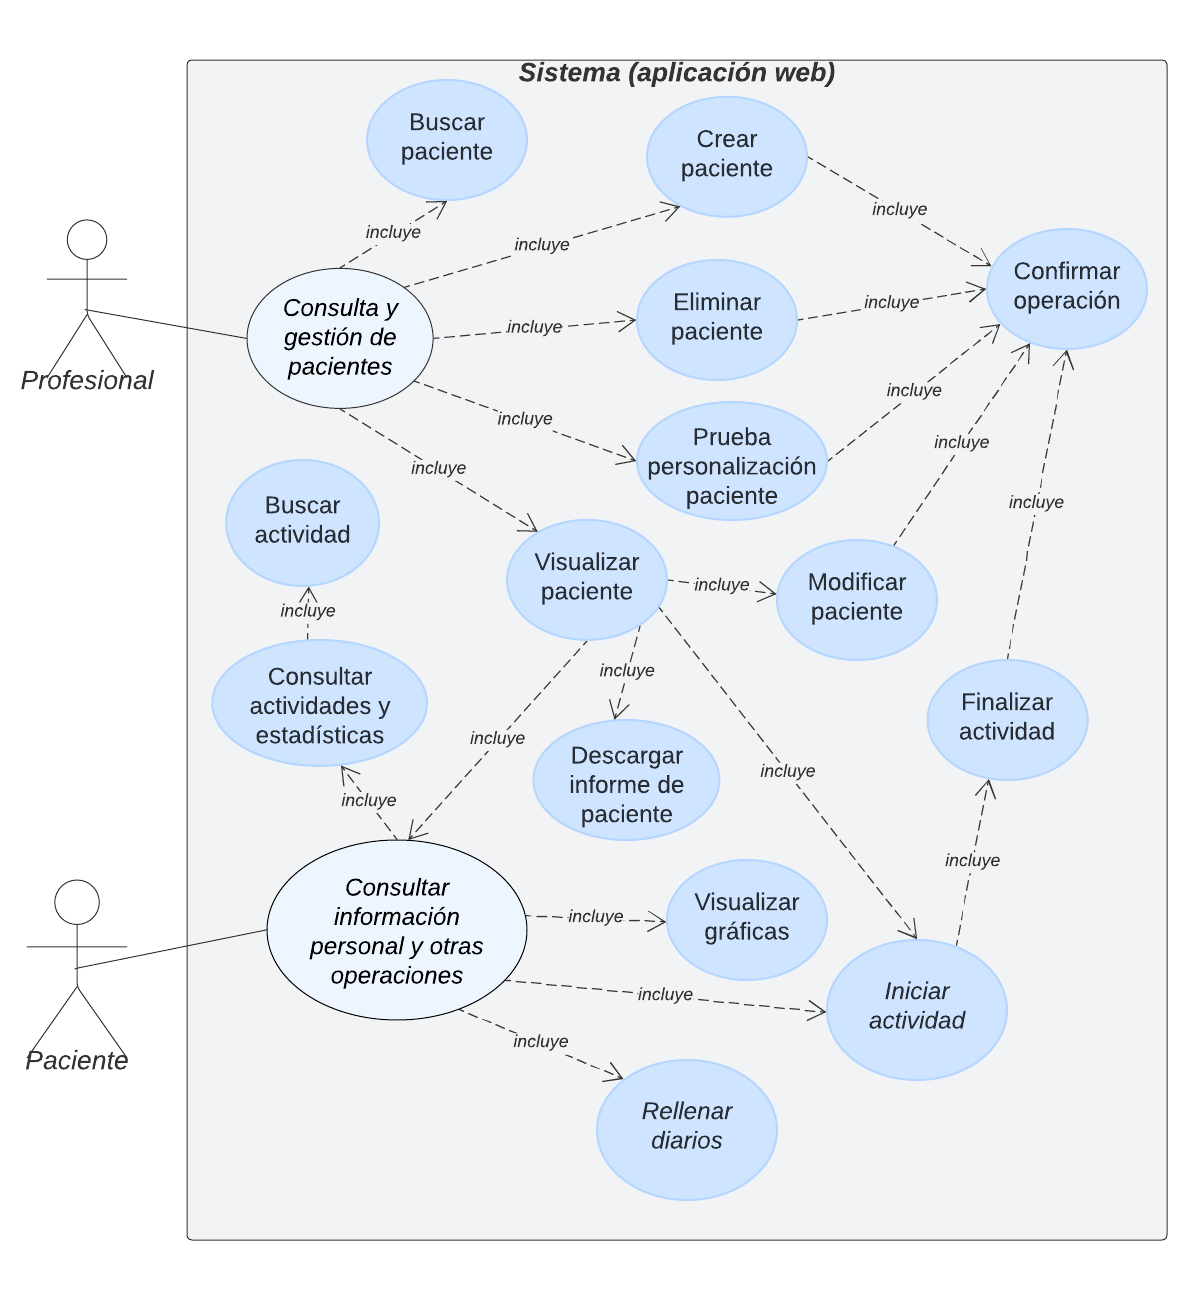
\includegraphics[width=1\textwidth]{img/casospacienteprof.png}
    \caption{Casos de uso para usuarios de tipo 'Profesional' y 'Paciente'. Fuente propia}
    \label{fig:Casospacienteprof}
\end{figure}

\section{Explicación casos de uso.}
Los casos de uso relativos a funcionalidades nuevas de la app, mostrados en la figura \ref{fig:Casosdeuso}, se explican detalladamente en las siguientes tablas: \ref{tab:CU-1}, \ref{tab:CU-2}, \ref{tab:CU-3}, \ref{tab:CU-4}, \ref{tab:CU-5}, \ref{tab:CU-6}
Se puede describir mediante el uso de tablas o mediante lenguaje natural.    

% Caso de Uso 1 -> Consultar Experimentos.
\begin{table}[p]
	\centering
	\begin{tabularx}{\linewidth}{ p{0.21\columnwidth} p{0.71\columnwidth} }
		\toprule
		\textbf{CU-1}    & \textbf{Consulta de gráficas del paciente}\\
		\toprule
		\textbf{Versión}              & 2.0    \\
		\textbf{Autor}                & Carmen Marcos \\
		\textbf{Requisitos asociados} & RF-10 \\
		\textbf{Descripción}          & Acceso por parte del usuario de tipo 'paciente' o 'profesional' a las gráficas creadas a partir de los datos de las actividades registradas por el paciente y los datos de toma de medicaciones y fluctuaciones motoras registrados en los diarios del paciente \\
		\textbf{Precondición}         & El usuario hace click en el botón 'Ver gráficas' situado en la sección de consulta de actividades\\
		\textbf{Acciones}             &
		\begin{enumerate}
			\def\labelenumi{\arabic{enumi}.}
			\tightlist
			\item Se muestran en pantalla los nombres de las gráficas, junto con botones para mostrar/ocultar cada gráfica.
			\item Al pulsar en uno de los botones se muestra la gráfica correspondiente (pueden mostrarse varias gráficas en la pantalla simultáneamente en caso de pulsar varios botones).
                \item Al hacer click una segunda vez en alguno de los botones se ocultará la gráfica correspondiente.
		\end{enumerate}\\
		\textbf{Postcondiciones}        & Para mostrar cada tipo de gráfica de forma adecuada deben cumplirse unas postcondiciones diferentes:
  \begin{enumerate}
        \def\labelenumi{\arabic{enumi}.}
	\tightlist
      \item Gráficas de bloqueos totales y bloqueos por minuto en las actividades: Se requiere que se hayan almacenado datos de actividades previamente
      \item Gráfica de estado del paciente: Deben haber sido registrados en la misma fecha los diarios de toma de medicaciones y de fluctuaciones motoras.
      \item Gráfica de bloqueos por minuto en los diferentes estados (on, off, on con discinesia): Se han registrado datos de actividades y diarios de fluctuaciones motoras en fechas similares
  \end{enumerate}\\
		\textbf{Excepciones}          & Los datos necesaerios para la creación de gráficas no se encuentran almacenados en la base de datos \\
		\textbf{Importancia}          & Media \\
		\bottomrule
	\end{tabularx}
	\caption{CU-1 Consulta de gráficas del paciente.}
        \label{tab:CU-1}
\end{table}

\begin{table}[p]
	\centering
	\begin{tabularx}{\linewidth}{ p{0.21\columnwidth} p{0.71\columnwidth} }
		\toprule
		\textbf{CU-2}    & \textbf{Prueba de personalización}\\
		\toprule
		\textbf{Versión}              & 2.0    \\
		\textbf{Autor}                & Carmen Marcos \\
		\textbf{Requisitos asociados} & RF-08\\
		\textbf{Descripción}          & Prueba diseñada para personalizar los segundos consecutivos de reposo que el sensor MPU-6050 considerará como congelamiento de la marcha. El usuario 'profesional' tiene acceso a la misma, pretendiendo que en una primera cita de explicacion y puesta en marcha de la solución tecnológica pueda asistir al paciente durante la realización de la prueba. 
        %Los resultados de la prueba se guardarán en la tabla 'personalización' de la base de datos. Esta actividad no percibe episodios de congelamiento de la marcha, teniendo como único objetivo obtener una idea significativa de los segundos que tarda el usuario en dar 1 paso, a partir de los cuales se calculará posteriormente mediante una fórmula el número personalizado de segundos. 
        \\
		\textbf{Precondición}         & El profesional hace click en el botón 'consultar' situado en la tabla de pacientes para llegar al apartado de información del paciente correspondiente. Posteriormente, hace click en el botón 'personalización', redirigiéndose a la pantalla de realización de prueba.
		\\
		\textbf{Acciones}             & \begin{enumerate} \def\labelenumi{\arabic{enumi}.}
	\tightlist
		\item Se mostrarán los botones 'iniciar actividad' y 'volver al menú'
        \item Al pulsar el botón 'iniciar actividad' se mostrarán en pantalla los datos (pasos, velocidad, duración), al igual que en una actividad normal.
        \item Al sobrepasar los 10 pasos de actividad, se muestra un botón de 'finalizar actividad'%ya que se considera la actividad realizada una muestra válida para el cálculo del tiempo medio que transcurre en cada paso.
        \item Al pulsar el botón 'finalizar actividad' se mostrará en pantalla el número de segundos personalizado que se ha calculado, así como un mensaje de confirmación que preguntará al usuario si se desean guardar los datos.
        \item En caso afirmativo, se guardarán los datos en la tabla 'personalización' de la base de datos.
		\end{enumerate}\\
		\textbf{Postcondiciones}        & 		El dispositivo se encuentra conectado mediante bluetooth al dispositivo correspondiente. El archivo bridge.py y el servidor node.js están ejecutándose para establecer comunicación bidireccional entre el dispositivo y la página web. %Estos archivos deben haber sido activados ejecutando el primero y escribiendo node server.js en la terminal desde el directorio del segundo.
  \\
		\textbf{Excepciones}          & Los archivos bridge.py y server.js no funcionan adecuadamente o no se establece una conexión bluetooth adecuada con el dispositivo. \\
		\textbf{Importancia}          & Alta \\
		\bottomrule
	\end{tabularx}
	\caption{CU-2 Prueba de personalización.}
        \label{tab:CU-2}
\end{table}

\begin{table}[p]
	\centering
	\begin{tabularx}{\linewidth}{ p{0.21\columnwidth} p{0.71\columnwidth} }
		\toprule
		\textbf{CU-3}    & \textbf{Asignar pauta de medicación a un paciente}\\
		\toprule
		\textbf{Versión}              & 2.0    \\
		\textbf{Autor}                & Carmen Marcos \\
		\textbf{Requisitos asociados} & RF-03 \\
		\textbf{Descripción}          & El usuario de tipo 'profesional' puede asociar a uno de sus pacientes asignados una pauta de medicación, especificando cuantas medicaciones relacionadas con síntomas motores del Párkinson deben tomar diariamente, cuáles y cuántas tomas en cada una.
        \\
		\textbf{Precondición}         & El usuario habrá iniciado sesión en la aplicación web utilizando una cuenta de tipo 'profesional' válida. El usuario pulsa el botón 'agregar pauta', situado en la pantalla de inicio.
		\\
		\textbf{Acciones}             & \begin{enumerate} \def\labelenumi{\arabic{enumi}.}
	\tightlist
		\item El usuario visualiza el formulario a rellenar, seleccionando el paciente para el cual desea agregar una pauta de medicación.
        \item El usuario selecciona el número de medicaciones distintas que deben ser tomadas durante el día. El contenido del formulario se adaptará dinámicamente a este número, mostrando tantos cuadros de medicación como sean necesarios.
        \item El usuario ajusta los nombres de las medicaciones y el número de tomas de cada una de ellas que deben realizarse cada día.
        \item Tras haber completado el formulario, el usuario pulsará el botón "guardar".
        \item Los datos se almacenarán en la tabla 'pautas' de la base de datos
		\end{enumerate}\\
		\textbf{Postcondiciones}        & 		No existen postcondiciones
  \\
		\textbf{Excepciones}          & No existen excepciones \\
		\textbf{Importancia}          & Media \\
		\bottomrule
	\end{tabularx}
	\caption{CU-3 Asignar pauta de medicación a un paciente.}
        \label{tab:CU-3}
\end{table}

\begin{table}[p]
	\centering
	\begin{tabularx}{\linewidth}{ p{0.21\columnwidth} p{0.71\columnwidth} }
		\toprule
		\textbf{CU-4}    & \textbf{Rellenar el diario de tomas de medicaciones}\\
		\toprule
		\textbf{Versión}              & 2.0    \\
		\textbf{Autor}                & Carmen Marcos \\
		\textbf{Requisitos asociados} & RF-09 \\
		\textbf{Descripción}          & El usuario de tipo 'paciente' puede acceder al diario de tomas de medicación de la fecha actual, un formulario en el que se especificarán las medicaciones relacionadas con síntomas motores del Párkinson tomadas a lo largo del día y las horas de toma.
        \\
		\textbf{Precondición}         & El usuario habrá iniciado sesión en la aplicación web utilizando una cuenta de tipo 'paciente' válida
		\\
		\textbf{Acciones}             & \begin{enumerate} \def\labelenumi{\arabic{enumi}.}
	\tightlist
		\item Se mostrará el formulario relativo al diario, mostrando en caso de estar disponible la pauta de medicación asignada por el profesional (número y nombre de medicaciones y número de tomas de cada una) como respuestas predeterminadas.
        \item El usuario selecciona el número de medicaciones distintas que han sido tomadas durante el día. El contenido del formulario se adaptará dinámicamente a este número, mostrando tantos cuadros de medicación como sean necesarios.
        \item El usuario ajusta los nombres de las medicaciones, el número de tomas de cada una de ellas y las horas de toma realizadas ese día.
        \item Tras haber completado el formulario, el usuario pulsará el botón "guardar".
        \item Los datos se almacenarán en la tabla 'diario2' de la base de datos
		\end{enumerate}\\
		\textbf{Postcondiciones}        & 		No existen postcondiciones
  \\
		\textbf{Excepciones}          & No existen excepciones \\
		\textbf{Importancia}          & Alta \\
		\bottomrule
	\end{tabularx}
	\caption{CU-4 Rellenar el diario de tomas de medicación.}
        \label{tab:CU-4}
\end{table}

\begin{table}[p]
	\centering
	\begin{tabularx}{\linewidth}{ p{0.21\columnwidth} p{0.71\columnwidth} }
		\toprule
		\textbf{CU-5}    & \textbf{Rellenar el diario de fluctuaciones motoras}\\
		\toprule
		\textbf{Versión}              & 2.0    \\
		\textbf{Autor}                & Carmen Marcos \\
		\textbf{Requisitos asociados} & RF-09 \\
		\textbf{Descripción}          & El usuario de tipo 'paciente' puede acceder al diario de fluctuaciones motoras de la fecha actual, un formulario en el que se especificarán los estados en que se encuentra el paciente a lo largo del día: ON, OFF, ON con discinesia o durmiendo. Se especificará el estado en intervalos de media hora desde las 7:00 hasta las 00:00.
        \\
		\textbf{Precondición}         & El usuario habrá iniciado sesión en la aplicación web utilizando una cuenta de tipo 'paciente' válida
		\\
		\textbf{Acciones}             & \begin{enumerate} \def\labelenumi{\arabic{enumi}.}
	\tightlist
		\item Se mostrará el formulario relativo al diario, constituido por una tabla que tiene las franjas horarias como filas y los estados como columnas, en que el paciente marcará para cada franja horaria el estado correspondiente haciendo click en la columna adecuada.
        \item Una vez que el usuario haya terminado de rellenar el formulario, pulsará el botón 'guardar'.
        \item Los datos se almacenarán en la tabla 'diario' de la base de datos
		\end{enumerate}\\
		\textbf{Postcondiciones}        & 		No existen postcondiciones, aunque el usuario no rellene todas las filas los datos correspondientes a las filas rellenadas podrán guardarse.
  \\
		\textbf{Excepciones}          & No existen excepciones \\
		\textbf{Importancia}          & Alta \\
		\bottomrule
	\end{tabularx}
	\caption{CU-5 Rellenar el diario de fluctuaciones motoras.}
        \label{tab:CU-5}
\end{table}


\begin{table}[p]
	\centering
	\begin{tabularx}{\linewidth}{ p{0.21\columnwidth} p{0.71\columnwidth} }
		\toprule
		\textbf{CU-6}    & \textbf{Descargar el informe del paciente}\\
		\toprule
		\textbf{Versión}              & 2.0    \\
		\textbf{Autor}                & Carmen Marcos \\
		\textbf{Requisitos asociados} & RF-11\\
		\textbf{Descripción}          & 
        \\
		\textbf{Precondición}         & El usuario habrá iniciado sesión en la aplicación web utilizando una cuenta de tipo 'profesional' válida
		\\
		\textbf{Acciones}             & \begin{enumerate} \def\labelenumi{\arabic{enumi}.}
	\tightlist
		\item Se pulsará en el botón 'Generar informe'
        \item Se seleccionará una de las opciones: con gráficas o sin gráficas
        \item Al pulsar en dicha selección se descargará de manera automática el pdf solicitado.
		\end{enumerate}\\
		\textbf{Postcondiciones}        & Existen datos en la base de datos relativos al paciente y actividades realizadas por el mismo.		
  \\
		\textbf{Excepciones}          & \\
		\textbf{Importancia}          & Baja \\
		\bottomrule
	\end{tabularx}
	\caption{CU-6 Descargar informe del paciente.}
        \label{tab:CU-6}
\end{table}
\section{Prototipos de interfaz o interacción con el proyecto.}

\begin{figure}[h]
    \centering
    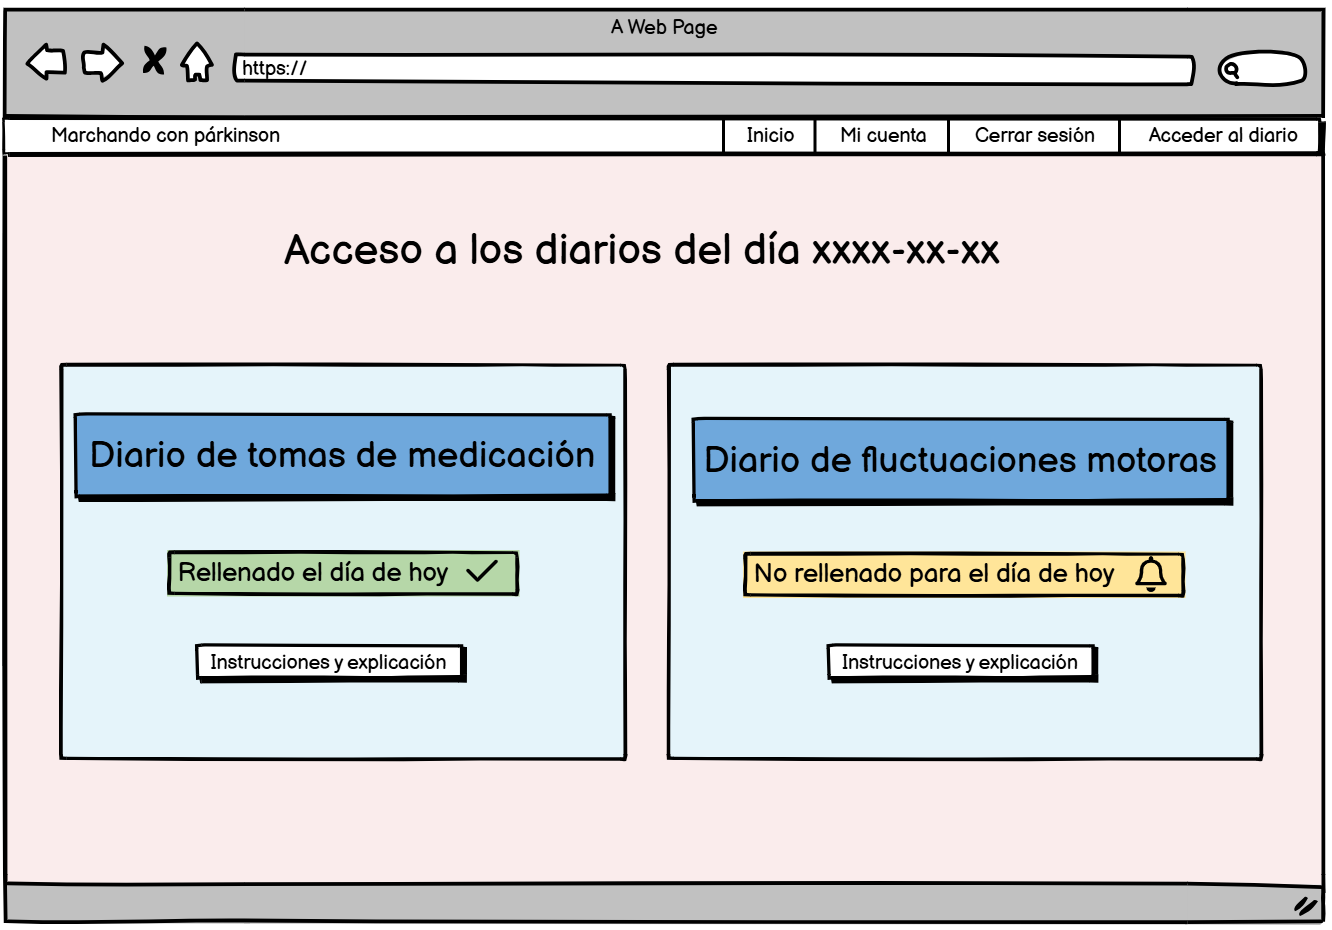
\includegraphics[width=1\textwidth]{img/wdiarios.png}
    \caption{Prototipo de interfaz para el acceso a diarios}
    \label{fig:Wireframediarios}
\end{figure}

\begin{figure}[h]
    \centering
    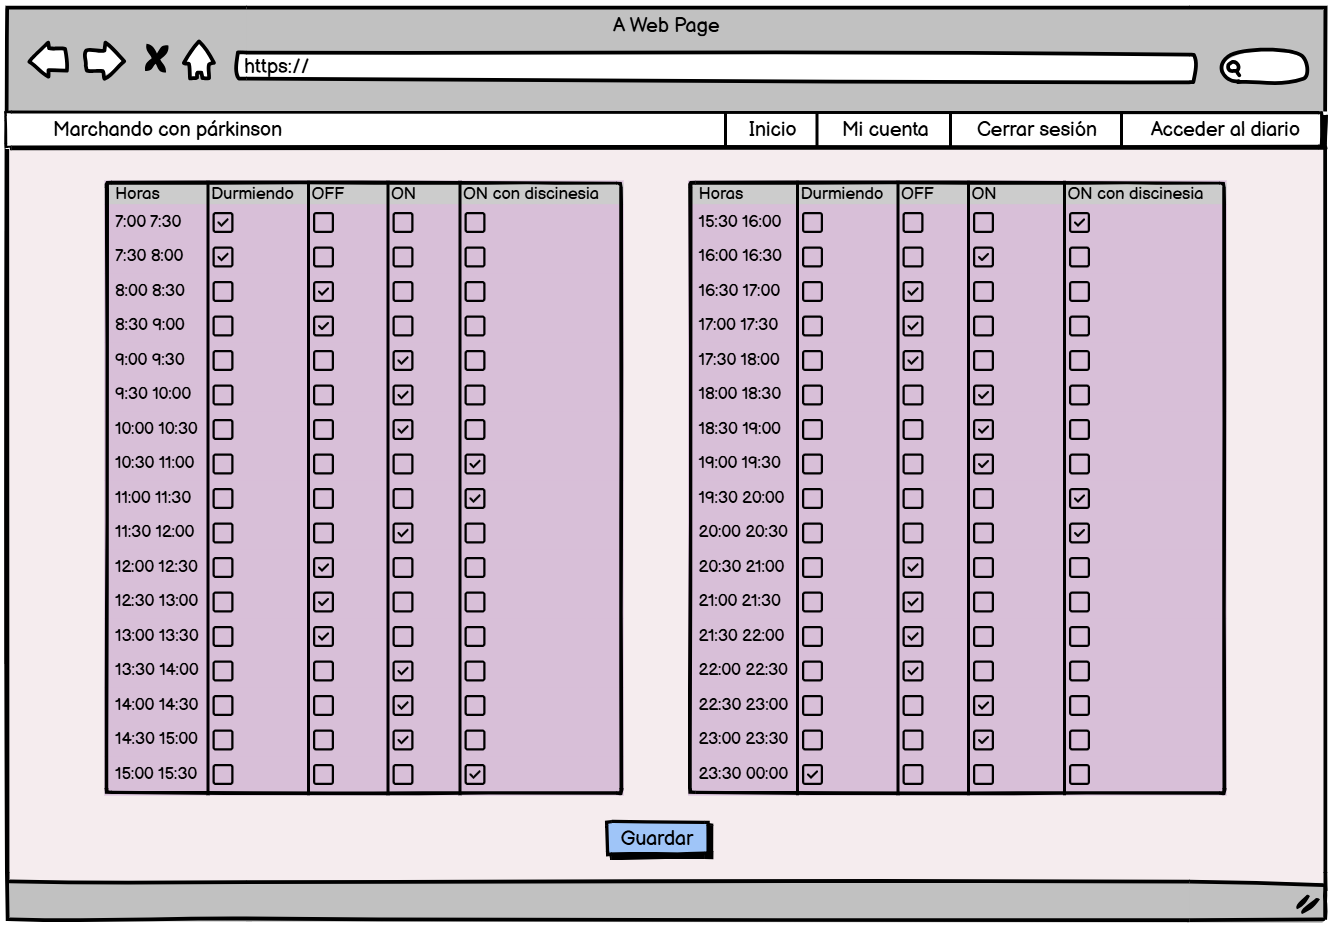
\includegraphics[width=1\textwidth]{img/wdiarioestados.png}
    \caption{Prototipo de interfaz para el diario de fluctuaciones motoras}
    \label{fig:Wireframeestados}
\end{figure}

\begin{figure}[h]
    \centering
    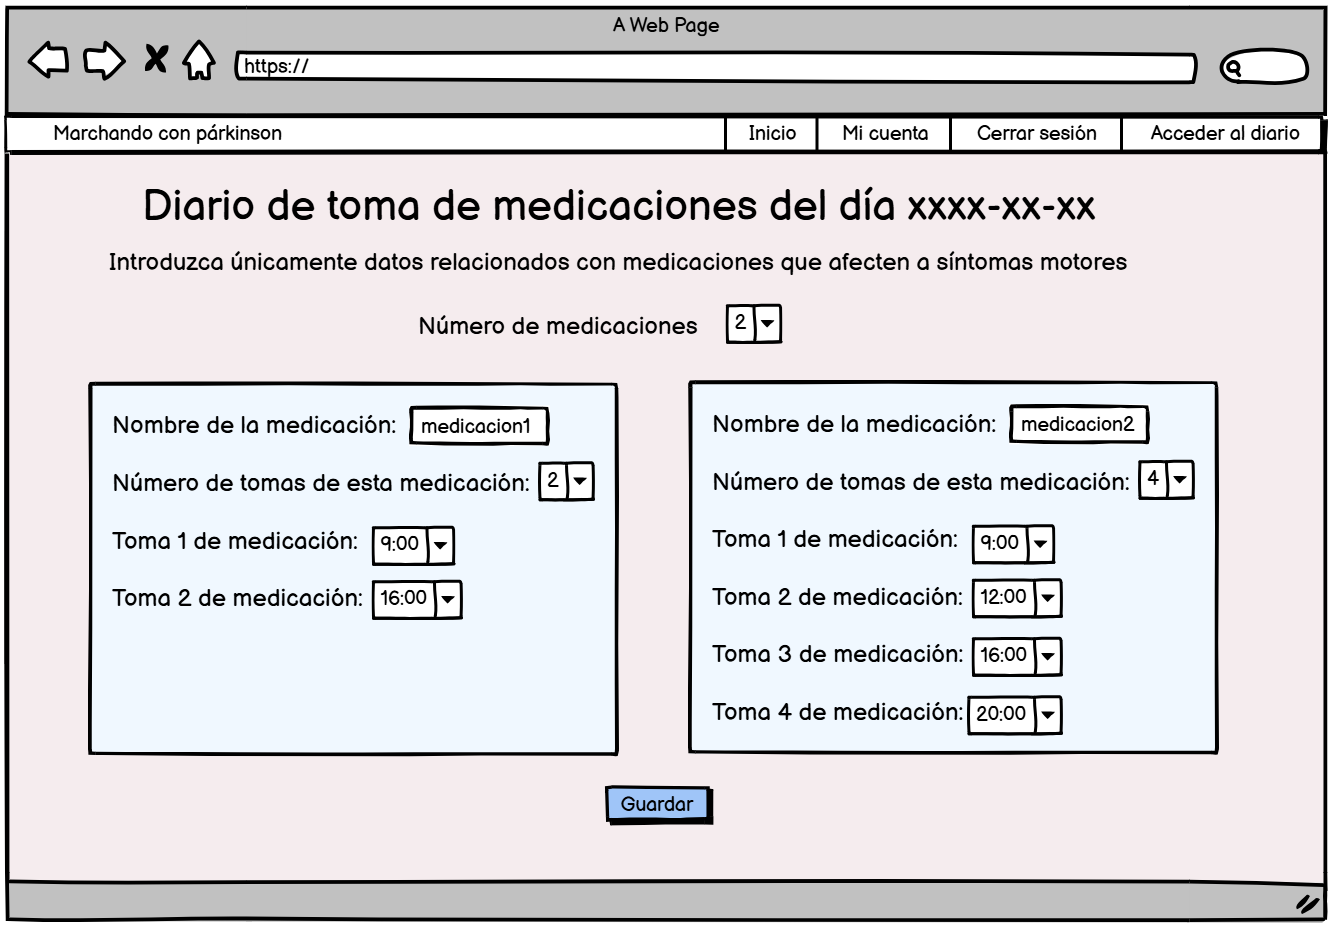
\includegraphics[width=1\textwidth]{img/wdiariotomas.png}
    \caption{Prototipo de interfaz para el diario de toma de medicaciones}
    \label{fig:Wireframemed}
\end{figure}

\begin{figure}[h]
    \centering
    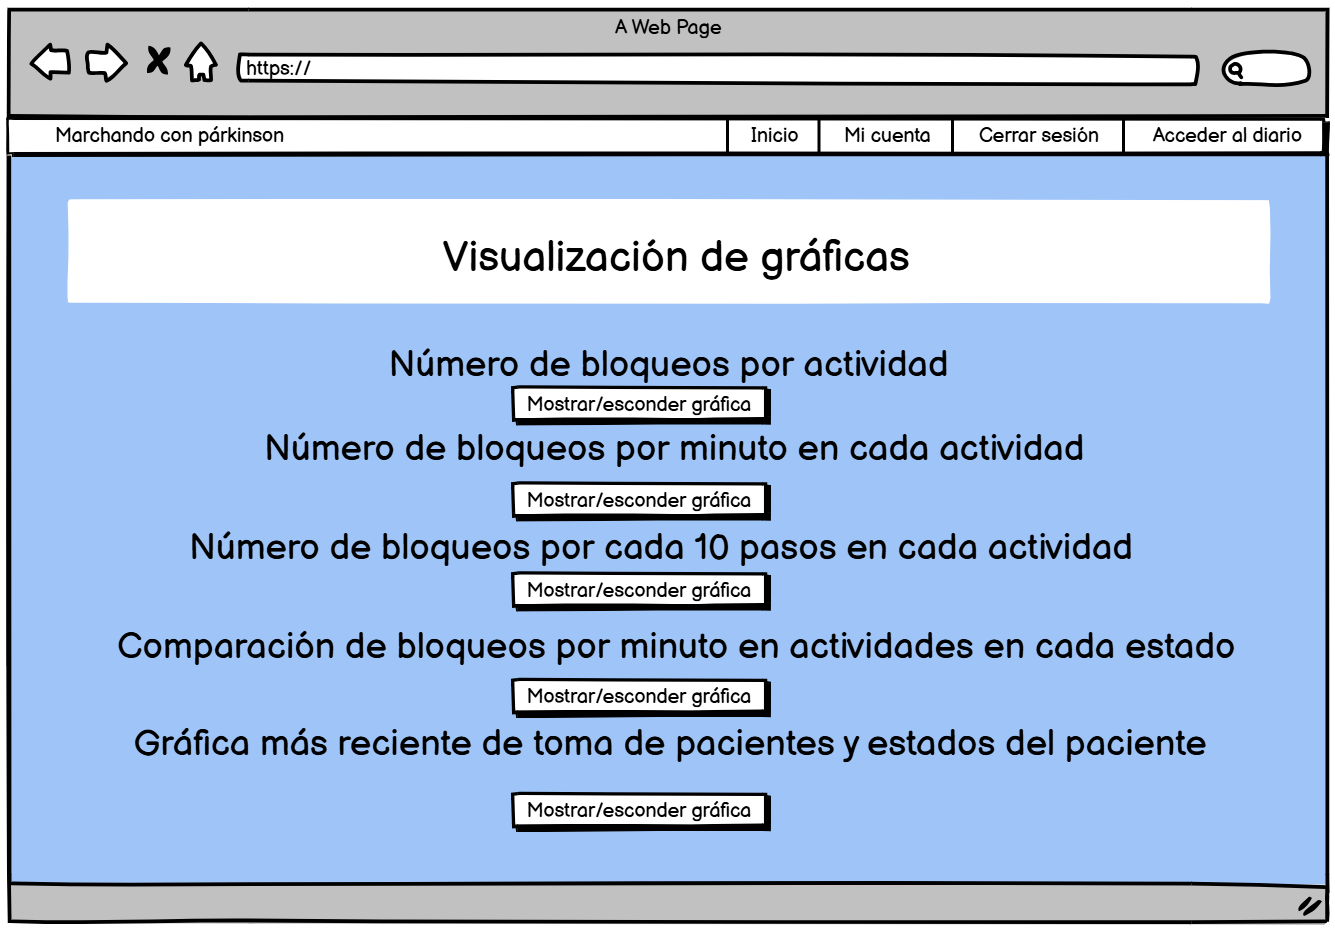
\includegraphics[width=1\textwidth]{img/wgraficas.png}
    \caption{Prototipo de interfaz para la visualización de gráficas}
    \label{fig:Wireframegraficas}
\end{figure}

\apendice{Estudio experimental}
John Brooke describe en 1996 una escala de usabilidad barata que puede ser utilizada para la evaluación global de la usabilidad de sistemas: la escala SUS (System Usability Scale) \cite{inbook}. Se trata de una escala Likert con 10 puntos claves para que indivíduos que hayan probado el sistema evalúen la usabilidad general del mismo.

Los indivíduos responden con una cifra del 1 al 5 (1 expresando completo desacuerdo y 5 expresando completo acuerdo) a 10 afirmaciones:
\begin{enumerate}
    \item Me gustaría utilizar el sistema de forma frecuente
    \item El sistema me parece innecesariamente complejo
    \item Creo que el sistema es fácil de utilizar
    \item Creo que necesitaría apoyo de personal técnico para poder utilizar el sistema
    \item Encuentro las diferentes funciones del sistema bien integradas
    \item Creo que hay demasiadas incosistencias en el sistema
    \item Imagino que la mayoría de gente aprendería a utilizar el sistema muy rápidamente
    \item Encuentro la utilización del sistema muy incómoda
    \item Me sentí muy confiado utilizando el sistema
    \item Necesité aprender muchas cosas antes de poder utilizar el sistema
\end{enumerate}
\section{Detalle de resultados.}
Con el objetivo de evaluar la usabilidad de la solución tecnológica propuesta para pacientes con Párkinson y profesionales, se realizó una demostración del funcionamiento del software y hardware en la Asociación de Párkinson de Burgos. Posteriormente, se envió a los profesionales de dicha asociación que habían presenciado la demostración una encuesta SUS (System Usability Scale) realizada mediante Google Forms para obtener un primer feedback proveniente de personal especializado.

La encuesta fue rellenada por un profesional de la salud de la asociación, obteniendo los siguientes resultados\ref{fig:encuesta1} \ref{fig:encuesta2} \ref{fig:encuesta3}:
    \begin{figure}[h]
        \centering
        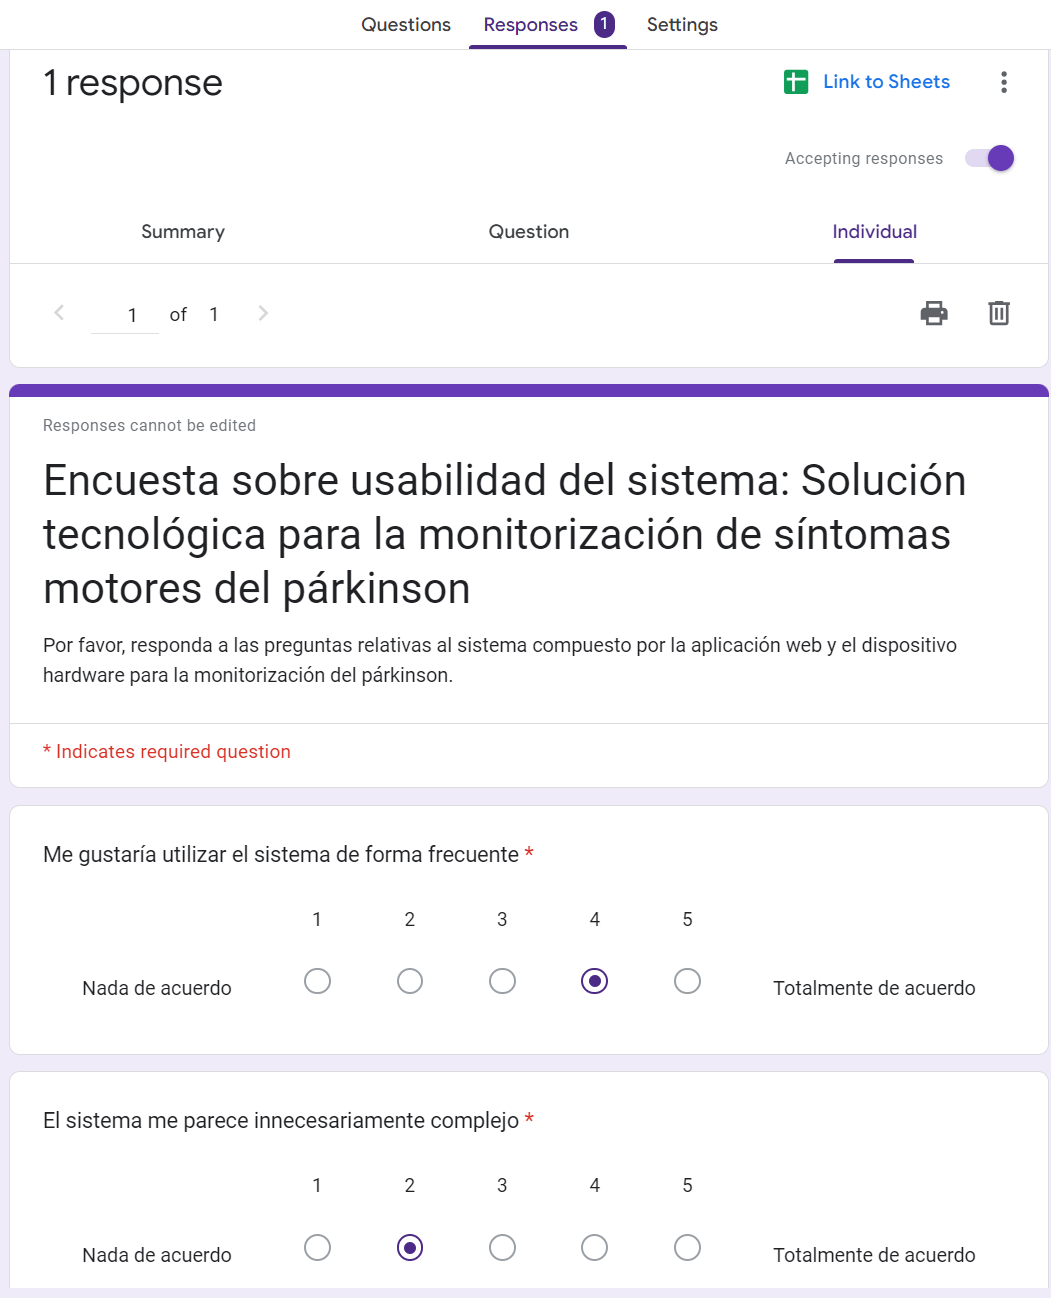
\includegraphics[width=1\textwidth]{img/encuesta1.png}
        \caption{Resultados de la encuesta SUS, parte 1. Fuente propia.}
        \label{fig:encuesta1}
    \end{figure}
        \begin{figure}[h]
        \centering
        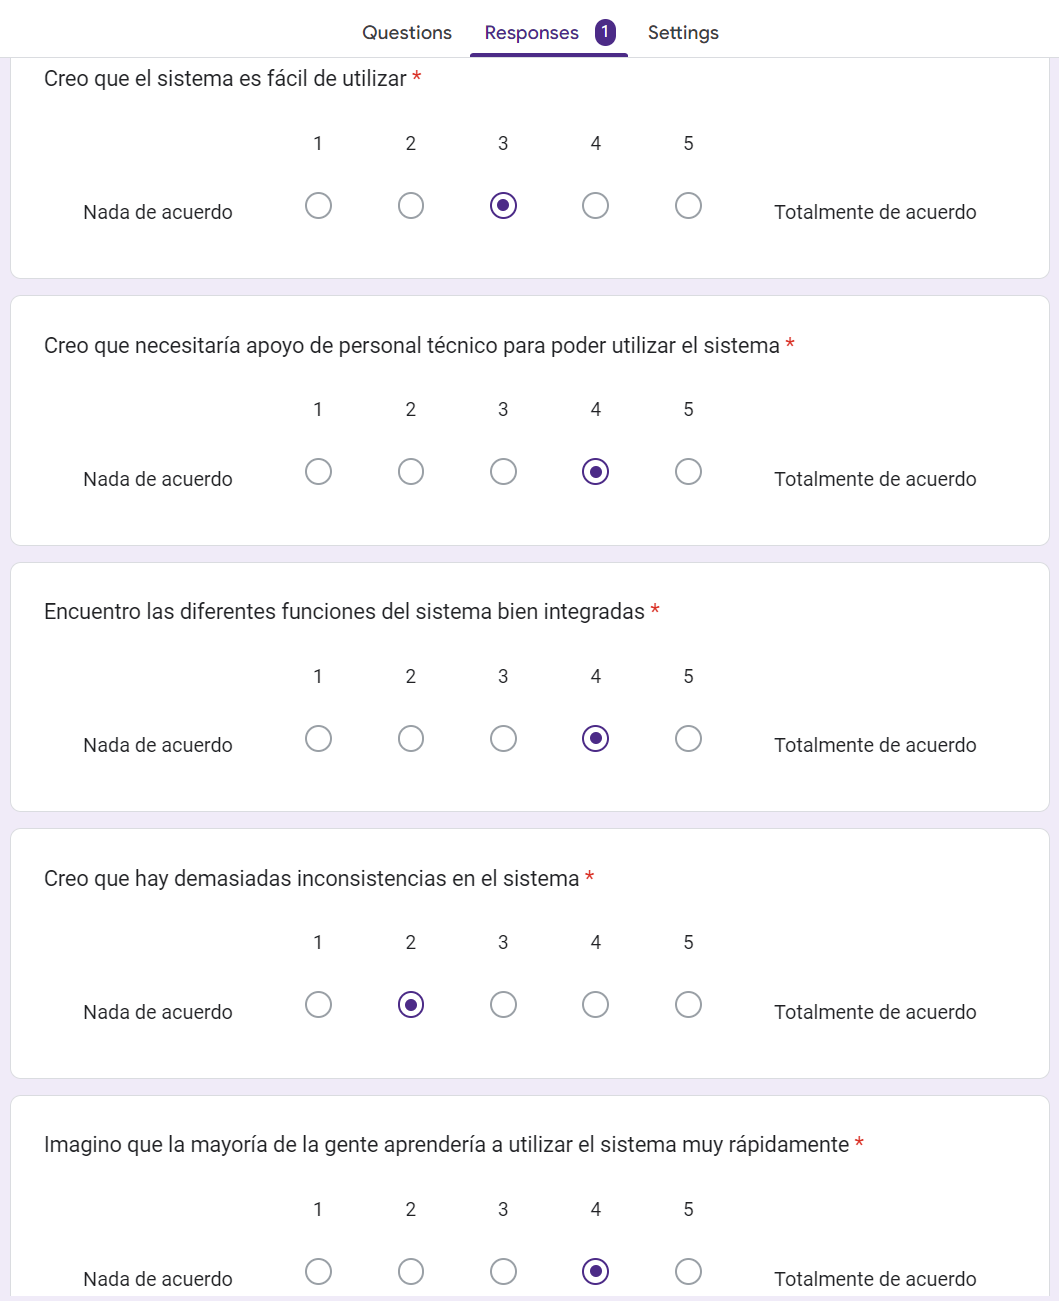
\includegraphics[width=1\textwidth]{img/encuesta2.png}
        \caption{Resultados de la encuesta SUS, parte 2. Fuente propia.}
        \label{fig:encuesta2}
    \end{figure}
        \begin{figure}[h]
        \centering
        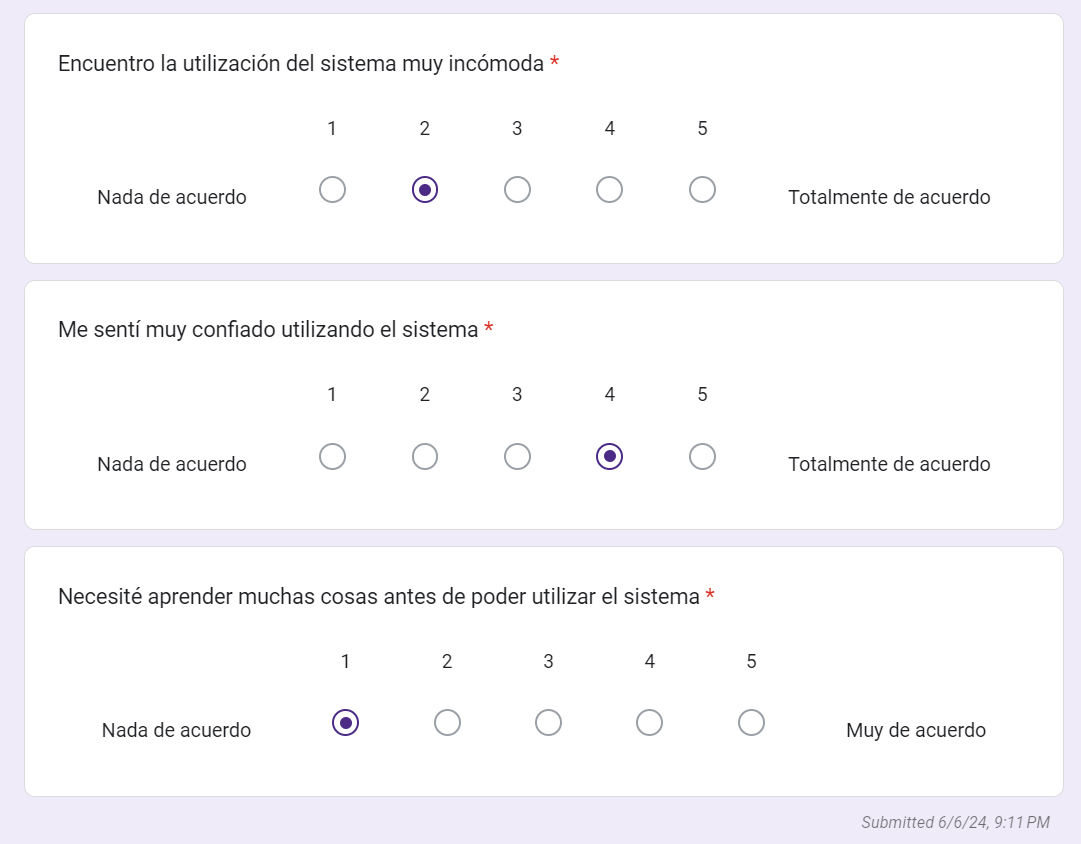
\includegraphics[width=1\textwidth]{img/encuesta3.png}
        \caption{Resultados de la encuesta SUS, parte 3. Fuente propia.}
        \label{fig:encuesta3}
    \end{figure}
Tal y como observamos en el artículo \cite{kaya2019usability}, el cálculo del 'score' o puntuación de una encuesta SUS se realiza de la siguiente forma:
\begin{enumerate}
    \item La puntuación correspondiente a las respuestas a preguntas impares (positivas), se calculan restando 1 al resultado obtenido. En este caso los resultados de la encuesta son 4, 3, 4, 4 y 4; por lo cual obtendríamos los números 3,2,3,3 y 3. La suma de estas puntuaciones es 14.
    \item La puntuación correspondiente a las respuestas a preguntas pares (negativas), se calcula restando al número 5 el resultado obtenido, es decir, con los resultados de la encuesta 2,4,2,2 y 1 obtendríamos los números 3,1,3,3 y 4. La suma de estas puntuaciones es 14.
    \item Para obtener la puntuación final (del 0 al 100), multiplicaremos por 2.5 la suma de ambas puntuaciones, es decir (14+14)*2.5 = 70.
\end{enumerate}
En el artículo \cite{sauro2016quantifying}, se establece 68 como puntuación media en encuestas SUS, teniendo una desviación estandar de 12.5. Como podemos observar en la tabla \ref{fig:sus}, la puntuación obtenida (70 puntos), se sitúa por encima del 56 por ciento de los sistemas analizados con esta escala. Esto refleja una relativa aceptabilidad del sistema, presentando también un ámplio rango de mejora en la facilidad de uso del mismo. En particular, el enunciado en el cual se obtuvo una respuesta más negativa fue 'Creo que necesitaría apoyo de personal técnico para poder utilizar el sistema'.

Es necesario tener en cuenta que estos resultados tienen una validez limitada, debido a que se obtuvieron a partir de las respuestas de un sólo participante. Sin embargo, teniendo en cuenta la similar reacción de todos los profesionales de la asociación de Párkinson que presenciaron la demostración y que el presente producto es tan sólo un prototipo, esta evaluación es suficiente para obtener una primera idea sobre qué puntos deberían mejorarse en futuras versiones del prototipo.
        \begin{figure}[h]
        \centering
        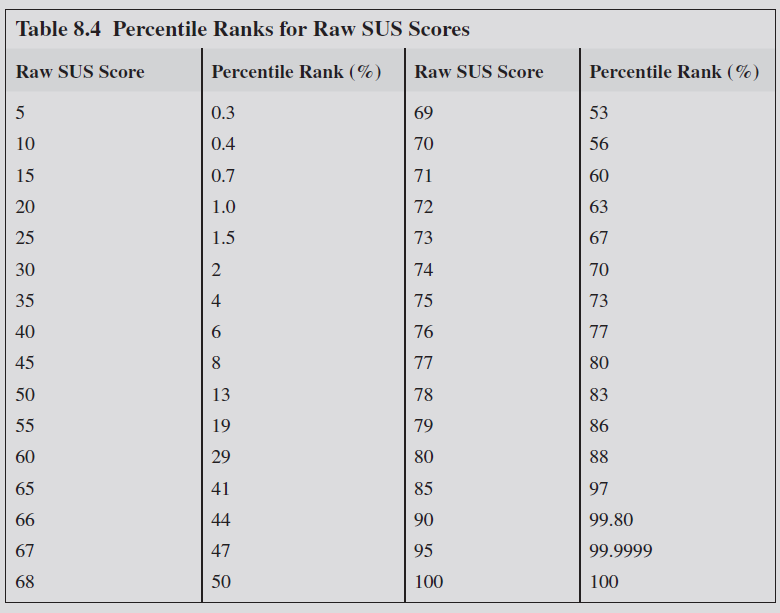
\includegraphics[width=1\textwidth]{img/sus.png}
        \caption{Tabla relacionando puntuaciones SUS con el rango de percentils percentiles \cite{sauro2016quantifying}.}
        \label{fig:sus}
    \end{figure}
\apendice{Anexo de sostenibilización curricular}

El grado en Ingeniería de la Salud, a partir del cual se presenta el presente Trabajo de Fin de Grado está alineado de manera natural con el respeto a los derechos fundamentales de las personas, ya que el desarrollo de software y/o hardware para complementar el tratamiento sanitario garantiza el acceso al sistema sanitario de personas en áreas rurales, con pocos recursos económicos o situados en zonas con baja calidad en la atención sanitaria. 

Este respeto al derecho a la salud de todas las personas se entrelaza también con el respeto a la igualdad de trato y no discriminación, promoviendo la inclusión social de personas que padecen enfermedades incapacitantes o discapacidades mediante el diseño de soluciones personalizadas que adapten el acceso a su entorno a las necesidades de estas personas.

El presente proyecto pretende aplicar estos principios proporcionando una ayuda a personas con Párkinson y los profesionales que los atienden, manteniendo al mismo tiempo un compromiso con la sostenibilidad del producto mediante la cuidadosa elección de los componentes hardware. A continuación se detalla la forma de cumplimiento de estos derechos y obligaciones:
\begin{itemize}
    \item Cumplimiento del respeto a los derechos humanos o derechos fundamentales: El presente proyecto se alinea con el derecho a la salud, aportando una solución accesible y barata para la monitorización de síntomas motores en pacientes con párkinson. Garantizar esta monitorización permite hacer la actuación del profesional sanitario más efectiva, ya que le proporciona información muy relevante para la toma de decisiones médicas.
    \item Cumplimiento del respeto a la igualdad de género, igualdad de trato y no discriminación: Esta solución tecnológica pretende garantizar un simple manejo de la aplicación web, haciéndola accesible a todas las personas independientemente de su edad, género, formación... Adicionalmente, promueve la inclusión social de personas con Párkinson, al ser una herramienta que contribuye a recibir un mejor trato, reduciendo los síntomas motores que a menudo provocan el aislameniento de estos pacientes.
    \item Compromiso con la sostenibilidad y concienciación con el cambio climático: El presente proyecto utiliza una serie de productos con una larga vida útil, incluyendo una fuente de alimentación recargable. Esto reduce la cantidad de resíduos generados durante el uso del dispositivo. Adicionalmente, durante la realización del prototipo componentes como la pantalla LCD, el sensor MPU-6050 y la placa Arduino no se soldaron de forma directa a los cables del circuito, permitiendo la reutilización de los mismos cuando el dispositivo deje de ser útil o quiera rediseñarse.
\end{itemize}




\printbibliography
\end{document}